% -*- coding: utf-8; -*-
\documentclass[english,submission]{programming}
\usepackage{hyperref} 
\usepackage{tikz}
\usepackage{xcolor}
\usepackage{eurosym}
\usepackage{listings}
\lstset{
	basicstyle=\ttfamily\small,
	keywordstyle=\color{blue!70!black}\bfseries,
	commentstyle=\color{gray},
	stringstyle=\color{teal!80!black},
	backgroundcolor=\color{gray!8},
	frame=single,
	framerule=0pt,
	rulecolor=\color{gray!25},
	breaklines=true,
	captionpos=b,
}
\usetikzlibrary{shapes.geometric}
\usepackage{tabularx} 
\usepackage[backend=bibtex]{biblatex}
\addbibresource{references.bib}

\lstdefinelanguage{Rust}{
	keywords={async, pub, trait, fn, self, impl, let, mut, use, struct, enum, match, if, else, return, true, false},
	keywordstyle=\color{blue!70!black}\bfseries,
	comment=[l]{//},
	commentstyle=\color{gray},
	stringstyle=\color{teal!80!black},
	sensitive=true,
}



\title{A Privacy-First Operating System with Integrated Knowledge Infrastructure}
\subtitle{Design, Architecture, and Philosophy}
\titlerunning{A Privacy-First OS with Integrated Knowledge Infrastructure}

\author{Tim Jochen Kicker}
\affiliation{University of Innsbruck, Austria}

\keywords{operating system, knowledge graph, privacy, user sovereignty, AI integration, Linux}

\begin{document}

\maketitle

\begin{abstract}
Linux is already a capable, secure, and privacy-respecting foundation for a
desktop operating system. What it lacks is integration: applications store data
in isolation, there is no cross-application query layer, and making a modern
Linux desktop accessible and coherent for non-technical users remains an
unsolved problem. This work presents the design and architecture of a
Linux-based desktop operating system that addresses this gap without
compromising the properties that make Linux worth building on.

At its core is a structured, local-first Knowledge Graph that records system
activity as typed nodes and relationships, queryable across application
boundaries and time. All system components (applications, background services,
and an optional AI daemon etc.) access the graph through a single privileged daemon
using cryptographically scoped capability tokens, with no component holding
elevated trust by default.

The design is organized around five non-negotiables: local data by default,
zero telemetry, full offline operation, least-privilege permissions throughout,
and security that does not compromise usability. This work covers the full
system stack from the Wayland compositor and application framework through the
event infrastructure, permission model, profile isolation, and security
architecture, including an explicit threat model and honest treatment of the
limits of the proposed mitigations.

The system is currently in the design and planning phase. The contribution of
this work is the architecture itself: a concrete, implementable blueprint for a
privacy-preserving Linux desktop that treats the Knowledge Graph as
infrastructure rather than a feature.
\end{abstract}

\tableofcontents

%% Sections
\section{Introduction}
\label{sec:introduction}

\subsection{Motivation}
\label{sec:motivation}

Most Linux distributions are either conservative remixes of existing systems or
highly opinionated tools for a specific niche. Neither describes this project.

The dominant desktop operating systems have a structural problem. Windows works
against its own users: forced updates, advertisements in the start menu, and
background telemetry that nobody enabled and cannot be fully disabled. The German
Federal Office for Information Security (BSI) has studied this directly: as part
of the SiSyPHuS research programme, the BSI found that required diagnostic data
collection in Windows~10 and~11 runs continuously and cannot be turned off by
the user~\cite{bsi2022sisyphus}. macOS presents a different trade-off: its
privacy posture is meaningfully better than Windows, but the ecosystem is
deliberately constructed to keep users paying and dependent. A 2024 study
published at CHI found that even opting out of Apple's analytics during device
setup does not prevent data collection by individual system applications, and
that the setup process itself involves at least eight distinct data-sharing
decisions presented in ways that are not straightforward to review~\cite{kollnig2024apple}.
Every Linux distribution, however technically sound, has failed to reach people
who simply want to use a computer without becoming a system administrator. The
gap between technically capable and actually usable has not closed in thirty years.

This project exists to close that gap. It is a Linux-based operating system
designed around a different set of priorities: one that integrates a
system-wide knowledge graph, AI interfaces, and modern tooling not as features
bolted on top, but as foundational infrastructure. It takes a clear stance on
user sovereignty, independence from dominant platform vendors, and not being
annoying to use.
If an operating system is being built in 2025 anyway, there is no reason to
repeat patterns from 1995.

\subsection{Target Audience}
\label{sec:audience}

The primary audience is people switching from macOS or Windows who want a
genuinely good alternative: modern in appearance, functional out of the box,
and respectful of their autonomy. Consumer-first, not enterprise-first. The
macOS user tired of lock-in but unwilling to compromise on quality. The Windows
user whose computer feels like it belongs to Microsoft more than to them. They
do not want to configure. They want to arrive and work, and feel like the
operating system is actually theirs.

Business deployment is a supported use case. The architecture accommodates
managed environments and administrator policies. The user remains the primary
stakeholder regardless of deployment context: an administrator can configure
defaults and restrict software; an administrator cannot surveil users or
override their personal data ownership. The system is not enterprise-first;
it is user-first by design, in every context.

\subsection{Design Principles}
\label{sec:principles}

The following principles govern every design decision in this project. They are
not aspirational language; they are constraints that break ties and override
convenience.

The user's interests come first. No advertisements, no tracking, no dark patterns,
no telemetry without explicit consent. This applies in managed environments too:
an organization can configure and restrict, but cannot surveil. All system
intelligence runs locally. The knowledge graph, AI context, and activity history
do not leave the machine without an explicit user action. The system works fully
offline, without registration, and without depending on services controlled by
companies in other jurisdictions. Cloud features are opt-in extensions, not
prerequisites. This is a technical commitment. It means the architecture enforces
it, not just the privacy policy.

The system has to be genuinely good to use. Everything works on first boot. No
hunting for drivers, no reading wiki pages to get audio working. The interface
must look better than what users are coming from, because a poor interface is a
barrier to entry regardless of what is underneath it. Small things matter more
than large ones: a system that remembers what you were working on, or switches
themes everywhere in one action, earns trust faster than an impressive feature
nobody uses. Coherence matters too: shared configuration, shared theming, shared
interfaces across all components. No part of the system should look like it was
designed in a different decade by a different team.

New technology gets used when it makes sense, not because it is trending. AI
and the knowledge graph are here because they genuinely change what a personal
computer can do for the user. The goal is a useful, trustworthy system, not a
clean architecture. Where established standards exist, this project builds
compatibility bridges rather than replacements. Apps built for other Linux
desktops run here; standard hardware interfaces work; nothing is deliberately
broken for the sake of purity. The system can explain what it is doing, in
plain language, in a place the user can see and act on it.

\subsection{Positioning}
\label{sec:positioning}

Figure~\ref{fig:positioning} maps the design space along two axes: how easy
the system is to use for a non-technical user, and how much sovereignty the
user has over their own data and software environment. These two properties
have historically traded off against each other. Mainstream commercial systems
prioritize usability but compromise on sovereignty, typically through telemetry,
ecosystem lock-in, or both. The more privacy-conscious Linux distributions give
users genuine control but impose a real usability cost. The upper-right
quadrant, high usability \emph{and} high user sovereignty, is where this
project aims to land. No system targeting mainstream usability currently occupies it.

\begin{figure}[htbp]
\centering
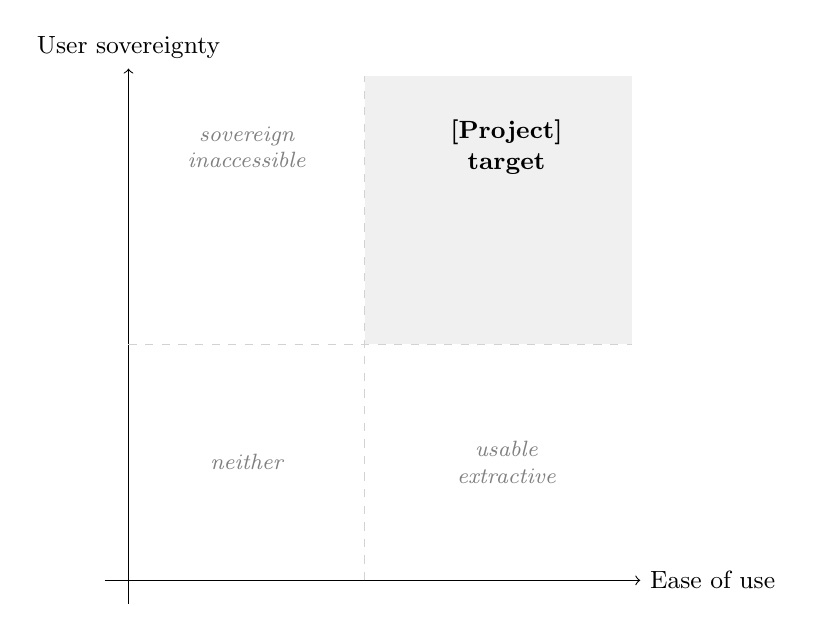
\begin{tikzpicture}
  % Axes
  \draw[->] (-0.3,0) -- (6.5,0)
    node[right, font=\small] {Ease of use};
  \draw[->] (0,-0.3) -- (0,6.5)
    node[above, font=\small] {User sovereignty};

  % Quadrant dividers
  \draw[gray!35, dashed] (3,0) -- (3,6.4);
  \draw[gray!35, dashed] (0,3) -- (6.4,3);

  % Target quadrant highlight
  \fill[gray!12] (3,3) rectangle (6.4,6.4);

  % Quadrant labels
  \node[gray, font=\footnotesize\itshape, align=center]
    at (1.5, 5.5) {sovereign\\inaccessible};
  \node[gray, font=\footnotesize\itshape, align=center]
    at (4.8, 1.5) {usable\\extractive};
  \node[gray, font=\footnotesize\itshape, align=center]
    at (1.5, 1.5) {neither};

  % Project target
  \node[font=\small\bfseries, align=center]
    at (4.8, 5.5) {[Project]\\target};

\end{tikzpicture}
\caption{Design space: ease of use versus user sovereignty. The shaded quadrant
is the project target. Mainstream commercial systems land in the lower-right
(usable but extractive); privacy-oriented Linux distributions in the upper-left
(sovereign but inaccessible). No mainstream system currently occupies the
upper-right.}
\label{fig:positioning}
\end{figure}

\subsection{What This Project Is Not}
\label{sec:nongoals}

Clarifying what this project is not is as important as describing what it is.

It is not a minimal system stripped to its essentials. There is real complexity
here, and that is intentional: a system that works for non-technical users
requires more infrastructure, not less.

It is not a fully declarative system where every piece of software is managed
through configuration files. Reproducibility is a goal; mandatory declarative
configuration is not.

It is not a distro aimed at advanced Linux users only. New users are explicitly
part of the target. Advanced users are welcome and well-served, but they are not
the primary design constraint.

It is not an enterprise product that happens to support consumers. The
design constraint is the non-technical user; business features exist where
they do not compromise that.

It is not a Windows or macOS clone. The goal is a better alternative, not a
familiar imitation.

\section{System Overview}
\label{sec:overview}

\subsection{Architecture at a Glance}
\label{sec:arch-glance}

The system is organized as a layered stack. Lower layers provide services to
higher layers; nothing reaches past its immediate neighbor. The bottom four
layers are always present: the OS base, the desktop environment, the messaging
and integration infrastructure, and the Knowledge Graph. Above those sit the
system's consumers: the applications, daemons, and optional AI daemon that
read from and write to the graph. Figure~\ref{fig:layers} shows the full
structure.

\begin{figure}[htbp]
\centering
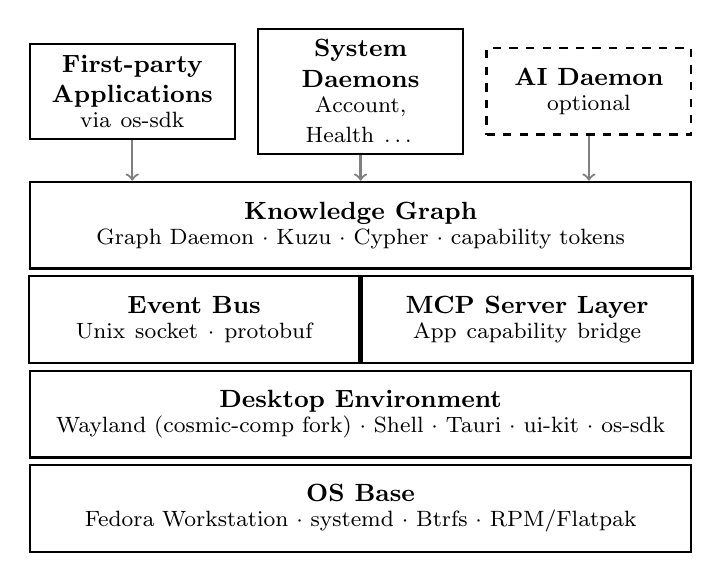
\begin{tikzpicture}[
	box/.style={
		draw, thick, rectangle,
		minimum width=8.4cm, minimum height=1.1cm,
		font=\small\bfseries, align=center, inner sep=5pt
	},
	splitbox/.style={
		draw, thick, rectangle,
		minimum width=4.2cm, text width=3.8cm, minimum height=1.1cm,
		font=\small\bfseries, align=center, inner sep=5pt
	},
	tribox/.style={
		draw, thick, rectangle,
		minimum width=2.6cm, text width=2.3cm, minimum height=1.1cm,
		font=\small\bfseries, align=center, inner sep=4pt
	},
	optbox/.style={
		draw, thick, dashed, rectangle,
		minimum width=2.6cm, text width=2.3cm, minimum height=1.1cm,
		font=\small\bfseries, align=center, inner sep=4pt
	},
	arr/.style={->, thick, gray},
	]
	\def\sep{1.2}
	
	\node[box] (os) at (0, 0) {
		OS Base\\[-2pt]
		{\mdseries\footnotesize Fedora Workstation $\cdot$ systemd $\cdot$ Btrfs $\cdot$ RPM/Flatpak}
	};
	\node[box] (de) at (0, \sep) {
		Desktop Environment\\[-2pt]
		{\mdseries\footnotesize Wayland (cosmic-comp fork) $\cdot$ Shell $\cdot$ Tauri $\cdot$ ui-kit $\cdot$ os-sdk}
	};
	\node[splitbox, anchor=east] (eb)  at (0.0, 2*\sep) {
		Event Bus\\[-2pt]
		{\mdseries\footnotesize Unix socket $\cdot$ protobuf}
	};
	\node[splitbox, anchor=west] (mcp) at (0.0, 2*\sep) {
		MCP Server Layer\\[-2pt]
		{\mdseries\footnotesize App capability bridge}
	};
	\node[box] (kg) at (0, 3*\sep) {
		Knowledge Graph\\[-2pt]
		{\mdseries\footnotesize Graph Daemon $\cdot$ Kuzu $\cdot$ Cypher $\cdot$ capability tokens}
	};
	
	% Top row at y=5.3 — boxes at x=-2.9/0/+2.9 fill exactly 8.4cm
	\node[tribox]  (apps)    at (-2.9, 5.3) {
		First-party\\Applications\\[-2pt]
		{\mdseries\footnotesize via os-sdk}
	};
	\node[tribox]  (daemons) at ( 0.0, 5.3) {
		System\\Daemons\\[-2pt]
		{\mdseries\footnotesize Account, Health \ldots}
	};
	\node[optbox]  (ai)      at ( 2.9, 5.3) {
		AI Daemon\\[-2pt]
		{\mdseries\footnotesize optional}
	};
	
	\draw[arr] (apps)    -- (kg.north -| apps);
	\draw[arr] (daemons) -- (kg.north);
	\draw[arr] (ai)      -- (kg.north -| ai);
	
\end{tikzpicture}
\caption{System layer structure. The bottom four layers are always present and
initialize in order from bottom to top. The top row shows the three classes of
graph consumer: first-party applications (connected via os-sdk), system daemons
(Account, Health, Audit, and others), and the AI daemon (dashed, optional). All
three connect to the Graph Daemon over a Unix socket with per-application
capability tokens; none of them bypasses the daemon or accesses Kuzu directly.
The AI daemon is not architecturally privileged over the others.}
\label{fig:layers}
\end{figure}

\subsection{Layer Responsibilities}
\label{sec:layer-responsibilities}

\paragraph{OS Base.}
The foundation is a standard Linux distribution providing the kernel, init
system, package manager, and base userspace tools. Nothing at this layer is
custom-built. The system builds on top of it; it does not replace it. The choice
of base distribution, the update strategy, and the concrete packages involved
are covered in detail in Section~\ref{sec:foundation}.

\paragraph{Desktop Environment.}
The Wayland compositor and the shell sit at this layer. This is what the user
directly interacts with: windows, the taskbar, the Waypointer launcher,
notifications, and the lock screen. All user-facing applications in this project
are built with \emph{Tauri}~\cite{tauri}, a framework described in
Section~\ref{sec:tauri-intro}. The compositor is based on a fork of
\emph{cosmic-comp}~\cite{cosmic:comp}, described in
Section~\ref{sec:compositor-intro}.

\paragraph{Event Bus.}
The internal message bus handles all communication between custom system
components. It receives, validates, and routes structured events from kernel
monitoring, the display system, and first-party applications. It runs as a
background service over \emph{Unix sockets} (see Section~\ref{sec:unix-sockets})
using \emph{Protocol Buffers} for schema-enforced serialization (see
Section~\ref{sec:protobuf}). Its role is purely to move and validate data; it
does not interpret or store anything.

\paragraph{MCP Server Layer.}
The \emph{Model Context Protocol}~\cite{mcp:spec} (MCP) is an open standard
published by Anthropic in 2024 for exposing application capabilities as callable
tools that AI models can invoke. In this system first-party applications expose
MCP servers as part of their standard implementation via os-sdk, giving any
MCP-compatible client a structured, permission-gated way to act on the system.
The MCP layer is not specific to the AI daemon; any client that implements the
protocol can use it.

\paragraph{Knowledge Graph.}
The graph database is the system's long-term memory: a local, structured index
of activity and context, queryable across time, application
boundaries, and data types. The \emph{Graph Daemon} is the sole reader and
writer of the underlying database; no other process opens the database files
directly. Every component that needs graph data connects to the daemon over a
Unix socket and presents a cryptographically signed capability token that encodes
its permitted query scope. Why a graph database rather than a relational one,
and why \emph{Kuzu}~\cite{kuzu} specifically, is explained in
Section~\ref{sec:kg-rationale}.

\paragraph{First-party applications.}
Every first-party application written for this system connects to the Graph
Daemon via the typed client bundled in \emph{os-sdk}. Opening the File Manager,
searching in Waypointer, or checking System Monitor all translate to parameterized
Cypher queries over a Unix socket. The application receives structured results
and renders them; it never touches the graph database files directly, and the
capability token it presents limits which node types and relations it can read.

\paragraph{System daemons.}
Background daemons such as the Account Daemon, Health Daemon, and Audit Daemon
are also graph clients. They write structured data into the graph (account
events, health observations, audit records) and read from it when their function
requires cross-domain context. Like applications, each daemon holds a
capability token with the minimum scope it needs; graph access is not elevated
for daemons by default.

\paragraph{AI daemon (optional).}
The AI daemon is a system daemon like the others. It connects to the Graph
Daemon via the same Unix socket interface, presents the same style of capability
token, and receives the same enforcement from the daemon. What distinguishes it
is not a privileged protocol position but a broader read permission at higher
user-configured access levels (see Section~\ref{sec:ai-security}). It
additionally orchestrates tool calls via the MCP layer and mediates between user
requests and model providers, local or cloud, behind a common Rust trait
interface (see Section~\ref{sec:rust-intro}). Disabling the AI daemon removes
AI features and nothing else; the graph, the applications, and the other daemons
are unaffected.

\subsection{Why Rust}
\label{sec:rust-intro}

All system daemons and Tauri application backends in this project are written in
\emph{Rust}, a systems programming language developed by Mozilla Research with
its 1.0 release in 2015. Understanding why requires a brief look at what systems
programming has historically looked like.

C and C++ have dominated operating system components, daemons, and
performance-critical software for decades. Their advantage is direct control
over memory and hardware with minimal overhead. Their liability is that this
control is entirely manual: the programmer allocates memory and is responsible
for freeing it correctly, without using it afterward, without reading past its
bounds, and without sharing it unsafely across threads. Memory safety bugs
(use-after-free, buffer overflows, data races) are the single largest source
of exploitable vulnerabilities in system software. Google's Project Zero and
Microsoft's Security Response Center have independently reported that roughly
70\% of serious security vulnerabilities in their codebases are memory safety
issues~\cite{msrc2019memory}.

Go is a more recent alternative with garbage collection and a simpler
concurrency model, but its garbage collector introduces unpredictable pause
latency unsuitable for low-level system components, and its runtime overhead is
significant compared to C or Rust.

Rust enforces memory safety through a compile-time ownership and borrowing
system. An entire class of bugs that would be exploitable vulnerabilities in C
simply cannot compile in Rust; the compiler rejects them. This is not a
runtime check with performance overhead; it is a zero-cost compile-time
guarantee. Rust has no garbage collector and achieves performance comparable to
C and C++.

For this project the consequence is concrete: every daemon runs continuously,
handles untrusted input from applications, and manages sensitive data including
credentials and graph queries. Writing them in Rust eliminates an entire
vulnerability class without sacrificing performance.

A \emph{Rust trait} is the language's mechanism for defining a shared interface
that multiple concrete types can implement, analogous to an interface in Java
or a pure abstract class in C++. When this document refers to the AI provider
abstraction as a Rust trait, it means that every AI backend implements the same
set of methods, and the rest of the codebase calls only those methods without
knowing which concrete backend is active at runtime.

\subsection{Why Wayland}
\label{sec:wayland-intro}

\emph{Wayland} is a display server protocol: the specification that defines how
applications communicate with the component responsible for drawing windows on
the screen.

\emph{X11} (the X Window System) was designed in 1984 and has been the
foundation of graphical Linux desktops ever since. Its architecture reflects its
era: the display server is a separate process, and by default any application
can inspect the input events and window contents of any other application on the
same display. One X11 application can read keystrokes typed into another
application's window. This is a keylogger-class capability that cannot be
removed without a protocol redesign, and it makes X11 structurally incompatible
with the isolation guarantees this project requires.

Wayland redesigns this from scratch: each application communicates only with the
compositor, not with other applications. Input events are delivered only to the
window that currently has focus. An application cannot read another
application's keystrokes or window contents. This isolation is the default
behaviour, not an optional hardening measure.

Wayland also has a cleaner model for multi-monitor and HiDPI configurations:
each output carries its own scale factor, and applications receive this
information directly and render at the correct resolution automatically.

The compatibility cost is real. Wayland addresses it through \emph{XWayland},
an X11 compatibility server that runs as a Wayland client. Legacy X11
applications work inside XWayland without modification. X11's security
limitations apply within the XWayland boundary but are contained there and do
not affect native Wayland applications.

\subsection{Why Tauri}
\label{sec:tauri-intro}

\emph{Tauri} is a framework for building desktop applications with a Rust
backend and a web-based user interface. A Tauri application consists of a Rust
process that handles system interactions, file access, and IPC, and a
\emph{WebView} that renders the UI using standard web technologies: HTML, CSS,
and TypeScript. The two halves communicate through a typed command bridge: the
frontend calls Rust functions via \texttt{invoke()}, and Rust pushes events to
the frontend via Tauri's event emitter. No ad-hoc serialization is needed; the
bridge handles it.

The dominant alternative is \emph{Electron}, which takes the same split but
bundles an entire Chromium browser and a Node.js runtime with every application.
A minimal Electron application ships roughly 150\,MB of runtime dependencies and
consumes around 300\,MB of RAM at idle. On a system with several Electron
applications running, the memory cost is substantial.

Tauri uses the operating system's existing WebView implementation instead of
bundling one. On Linux this is \emph{WebKitGTK}, the GTK port of the WebKit
rendering engine. WebKitGTK is already present on any modern Linux desktop; a
Tauri application does not add it. A Tauri application binary is typically
5--10\,MB and uses a fraction of the RAM that an equivalent Electron application
would require.

Building the UI in a native toolkit such as \emph{GTK4} or \emph{Qt} was
considered and rejected for two reasons. First, maintaining visual consistency
across components developed independently is significantly harder with a native
toolkit than with a shared CSS design system where a token change propagates
everywhere. Second, the developer pool for TypeScript and CSS is larger than
for GTK or Qt development, which matters for an open-source project expecting
community contributions. The trade-off is that WebView rendering is slightly
less efficient than native rendering for highly dynamic content, but this is not
a relevant concern for the settings panels, file browsers, and launchers that
make up this system's UI.

Tauri version 2.0, released in October 2024, is used throughout this project.
Version 2.0 introduced a revised permission system for Tauri commands (replacing
the allowlist model of 1.x with a finer-grained capability model), official
mobile support, and improved IPC ergonomics. The capability model in 2.0 aligns
well with this project's general approach to least-privilege permissions.

\subsection{Why cosmic-comp (Forked)}
\label{sec:compositor-intro}

The compositor is based on a fork of \emph{cosmic-comp}~\cite{cosmic:comp},
the Wayland compositor built by System76 for their COSMIC desktop environment.
cosmic-comp is written in Rust on top of \emph{Smithay}~\cite{smithay}, a Rust
library that provides the low-level compositor plumbing: Wayland protocol
handling, DRM/KMS interfaces for direct display hardware access, input
processing via \emph{libinput}, and buffer management including GPU-side
zero-copy paths via \texttt{dmabuf}.

\paragraph{Why fork rather than build from scratch.}
Building a production Wayland compositor from Smithay primitives is a
multi-year effort. cosmic-comp has already solved the hard problems: correct
multi-monitor handling with per-output scale factors, tiling and floating
window management, XWayland integration, screen capture via
\texttt{wlr-screencopy}, input method framework support for non-Latin input,
and the full Wayland protocol extension set a modern desktop requires. Forking
inherits all of this. Starting from scratch would reproduce it, worse, over a
longer timeline.

\paragraph{Why not adopt COSMIC wholesale.}
The COSMIC desktop ships as an integrated product: cosmic-comp is coupled to
cosmic-panel, cosmic-launcher, cosmic-settings, and the rest of the COSMIC
shell via custom Wayland protocol extensions and D-Bus interfaces designed
specifically for that stack. Adopting COSMIC wholesale would mean inheriting
its shell design, its theming system based on \emph{iced}, and its release
cadence -- none of which align with this project. The goal is the compositor
kernel, not the product.

\paragraph{What the fork retains.}
The fork keeps everything below the shell boundary: the Smithay-based window
management engine, the input pipeline, the multi-monitor and HiDPI
infrastructure, the XWayland bridge, and the Wayland protocol extension
implementations. Window placement logic, tiling and floating behaviour, focus
rules, and workspace management all come from cosmic-comp and are modified
only where this project's behaviour explicitly differs.

\paragraph{What the fork replaces.}
The entire shell layer is replaced. cosmic-comp's custom IPC protocols for
communicating with cosmic-panel and cosmic-launcher are removed. In their
place the compositor exposes the standard \texttt{wlr-} Wayland protocol
extensions -- \texttt{wlr-layer-shell}, \texttt{wlr-foreign-toplevel-management},
\texttt{wlr-workspace-management} -- which the Tauri-based shell consumes
exactly as any other compliant shell client would. A minimal custom Unix
socket channel handles events that have no standard Wayland equivalent: theme
updates, Focus Mode signals, and graph notifications from the Event Bus.
The shell is not a privileged internal component of the compositor; it is a
Wayland client with the same protocol access any shell would have.

\paragraph{Maintenance posture.}
The fork tracks cosmic-comp's upstream for bug fixes and Smithay version
updates. COSMIC-specific features that land upstream are evaluated
individually: those that improve the window management kernel are merged;
those that add COSMIC shell coupling are not. The fork is a maintained
derivative, not a snapshot.

\subsection{Component Boundaries}
\label{sec:component-boundaries}

The system's components divide into two categories: background services and
user-facing applications.

Background services are called \emph{daemons} in Unix terminology: processes
with no visible window that are started at boot by \emph{systemd} and
automatically restarted if they crash. systemd is the standard init system and
service manager on modern Linux distributions. It handles starting services in
dependency order at boot, logging their output to the journal, and enforcing
resource and sandboxing constraints via its service unit configuration. All
daemons in this project are written in Rust and run under tight systemd
sandboxing: each service unit declares exactly the filesystem paths, syscalls,
and network access it requires, and everything else is denied at the kernel
level.

\begin{table}[htbp]
\caption{Background services (daemons)}
\label{tab:daemons}
\begin{tabularx}{\linewidth}{lX}
\toprule
\textbf{Service} & \textbf{Responsibility} \\
\midrule
Event Bus       & Receives, validates, and routes internal events between components \\
Graph Daemon    & Sole reader/writer of the Knowledge Graph database \\
Account Daemon  & Credential management and login token handling \\
AI Daemon       & Model providers, MCP orchestration, graph queries (optional) \\
Module Runtime  & Manages the lifecycle of shell extensions \\
Transfer Daemon & Controls data movement between user profiles \\
Audit Daemon    & Sole writer to the append-only audit log \\
Health Daemon   & Aggregates and stores health and wellbeing data \\
Compositor      & Draws windows and manages the display (Wayland compositor) \\
\bottomrule
\end{tabularx}
\end{table}

User-facing applications are built with Tauri and share two common libraries,
described below; Table~\ref{tab:apps} lists them.

\begin{table}[htbp]
\caption{User-facing applications}
\label{tab:apps}
\begin{tabularx}{\linewidth}{lX}
\toprule
\textbf{Application} & \textbf{Notes} \\
\midrule
Shell        & Taskbar, Waypointer launcher, notification center, lock screen \\
Settings     & System-wide configuration: theming, permissions, AI level, accounts \\
File Manager & First-party file browser with graph-aware features \\
Store        & App and module discovery, installation, and updates \\
Terminal     & First-party terminal emulator with MCP integration \\
Wine Manager & Windows compatibility management UI \\
\bottomrule
\end{tabularx}
\end{table}

Every first-party application is built on two shared libraries. \emph{ui-kit}
is a TypeScript component library based on \emph{shadcn/ui} (a set of
accessible, unstyled components built on Radix UI primitives) styled with the
project's shared design token system using \emph{Tailwind CSS}. Tailwind is a
utility-first CSS framework where styles are applied via class names rather
than separate stylesheets; combined with CSS custom properties for design
tokens, a theme change propagates to all running applications without a
reload. \emph{os-sdk} is a Rust crate that provides ready-made clients for
the Graph Daemon and Event Bus, MCP server boilerplate, and the shared TOML
configuration system. A new first-party application starts with these two
libraries and has graph access, event emission, an MCP server, and a
consistent UI without writing any infrastructure code.

\subsection{Communication Model}
\label{sec:communication}

\subsubsection{Unix Sockets}
\label{sec:unix-sockets}

All inter-component communication uses \emph{Unix domain sockets}, a
communication mechanism built into the Linux kernel. A Unix socket behaves
like a network socket in its API but exists only on the local machine: it is
represented as a file path in the filesystem (for example
\texttt{/run/graph-daemon/graph.sock}), and only processes on the same machine
can connect to it. There is no network stack involved; data passes directly
through the kernel with latency in the range of a few microseconds.

D-Bus, the standard Linux IPC mechanism discussed in
Section~\ref{sec:dbus}, was not chosen for internal component communication:
it introduces a central broker process as an intermediary, adds marshalling
overhead, and its type system is not well suited to the structured binary
messages used here. TCP loopback sockets were also considered and rejected: they
go through the full network stack, carry more overhead, and expose a port
reachable by any process on the machine.

\subsubsection{Protocol Buffers}
\label{sec:protobuf}

Data transmitted over the internal sockets is serialized with \emph{Protocol
Buffers} (protobuf)~\cite{protobuf}, a binary serialization format developed and open-sourced by
Google. Serialization is the process of converting a data structure in memory
into a byte sequence for transmission, and deserialization is the reverse.

The alternative most developers reach for is JSON, a human-readable text format.
JSON has two disadvantages for a high-frequency internal bus. First, it carries
no schema: any JSON object is syntactically valid, so a receiver cannot
distinguish a malformed message from a valid one without application-level
checks. Second, text encoding is inefficient: a 64-bit integer written as its
decimal string representation takes 1--20 bytes; protobuf encodes the same value
in 1--10 bytes using variable-length encoding.

Protobuf defines message types in \texttt{.proto} schema files, which are
compiled to Rust code. A message that does not match the schema is rejected by
the generated parser before it reaches application logic, catching schema
violations at the boundary rather than deep inside a handler.

\emph{MessagePack} was considered as an alternative: it is a binary JSON
variant with compact encoding but no schema enforcement. \emph{Cap'n Proto} and
\emph{FlatBuffers} offer zero-copy deserialization and faster parsing for large
messages, but their Rust ecosystems are less mature than protobuf's. Protobuf
has the best combination of schema enforcement, Rust library quality, and
tooling.

\begin{table}[htbp]
\caption{Inter-component communication paths}
\label{tab:comms}
\begin{tabularx}{\linewidth}{lX}
\toprule
\textbf{Path} & \textbf{Transport} \\
\midrule
Daemon $\leftrightarrow$ Daemon            & Unix socket (protobuf) \\
App backend $\leftrightarrow$ Daemon       & Unix socket (protobuf) \\
App backend $\leftrightarrow$ App frontend & Tauri command bridge (typed) \\
Compositor $\leftrightarrow$ Shell         & Wayland protocols + Unix socket \\
\bottomrule
\end{tabularx}
\end{table}

A concrete example: a user action in the UI that queries the Knowledge Graph
follows this path:

\begin{center}
\texttt{UI event $\to$ App backend $\to$ Unix socket $\to$ Graph Daemon $\to$ Database}
\end{center}

Four steps, all local to the machine. The full round-trip is imperceptible to
the user.

\subsubsection{Knowledge Graph Rationale}
\label{sec:kg-rationale}

A relational database such as \emph{PostgreSQL} or \emph{SQLite} organizes data
into tables with rows and columns. Relationships between entities are expressed
as foreign key references and queried using \texttt{JOIN} operations, which
become progressively more expensive and harder to write as the number of hops
between entities increases.

A \emph{graph database} stores relationships as first-class data: entities are
\emph{nodes} and the connections between them are typed \emph{edges}, both with
their own properties. Traversing a relationship is a direct pointer follow,
not a table scan or index lookup. Querying "which files did the user work on
last Tuesday, via which applications, and are any of those applications still
running?" is a single graph traversal. In SQL it requires at minimum three joins,
a time-range filter, and a correlated subquery for the running-process check.

For an operating system where everything is connected (processes open files,
files belong to projects, projects span sessions, sessions involve multiple
applications), a graph is the natural data model.

\emph{Kuzu} is the query-facing graph database in this system. It is an embedded
graph database written in C++ with first-class Rust bindings, released under the
MIT license. \emph{Embedded} means it runs as a library inside the Graph Daemon
process with no separate server process, no network port, and no additional
service to manage. The database is a directory of files on disk that only the
Graph Daemon process opens.

Kuzu is an OLAP system: it is optimized for analytical queries over large graphs,
not for high-frequency transactional writes. This is a deliberate fit for its
role. The Graph Daemon uses a two-layer write architecture: \emph{SQLite} acts
as the high-frequency write store, accepting the continuous stream of eBPF
events and compositor events at full throughput. Structured, semantically
valuable data -- \texttt{UserAction} nodes, \texttt{Project} edges,
\texttt{Session} nodes -- is periodically promoted from SQLite into Kuzu, where
it becomes available for graph traversal queries. Raw eBPF noise never reaches
Kuzu; it is retained in SQLite for the anomaly detection window and then
discarded. This means Kuzu operates on a clean, curated graph rather than a
raw event log, which improves both query performance and the quality of AI
context.

The two layers have different retention windows and query surfaces. SQLite
answers time-range lookups over recent raw events; Kuzu answers multi-hop
graph traversals over semantic history. The Graph Daemon presents a unified
query interface to callers; the layer boundary is an implementation detail
they never see.

\emph{Neo4j} was evaluated and rejected. Neo4j is the most widely deployed
graph database and has a large ecosystem, but it runs as a separate server
process, its community edition has usage restrictions, and its JVM-based runtime
carries memory overhead inappropriate for a component embedded in a user session.

Kuzu uses \emph{Cypher} as its query language, an open graph query standard
(openCypher) originally developed for Neo4j. It reads close to natural language:

\begin{lstlisting}[language={}]
MATCH (f:File)-[:OPENED_BY]->(a:App)
WHERE f.last_modified > datetime('2026-03-01')
RETURN f.path, a.name
ORDER BY f.last_modified DESC
\end{lstlisting}

This query finds all files modified after a given date, which applications
opened them, and returns the results sorted by modification time.

\subsection{D-Bus Coexistence}
\label{sec:dbus}

\emph{D-Bus} is the standard inter-process communication system on Linux
desktops, in use since 2003. NetworkManager uses it to report network state
changes, BlueZ uses it for Bluetooth events, \texttt{systemd-logind} uses it
for session management, and the \emph{XDG Desktop Portal} uses it to give
sandboxed applications access to OS-level dialogs. It cannot be removed without
breaking the wider Linux software ecosystem.

D-Bus works as a message broker: a central \texttt{dbus-daemon} process routes
messages between senders and registered receivers identified by well-known bus
names such as \texttt{org.freedesktop.NetworkManager}. This model works well for
the ecosystem-level events it was designed for. The central broker and its
overhead make it a poor fit for the high-frequency structured events between
project-internal components, which is why the project uses its own Event Bus for
internal communication.

This system does not replace D-Bus. It runs alongside it. D-Bus remains
responsible for third-party application notifications via
\texttt{org.freedesktop.Notifications}, hardware events, portal interfaces, and
session management. The internal Event Bus handles communication between
project components only. The two systems are parallel and non-overlapping.

The rule for developers is simple: project-internal components communicate over
the internal Event Bus via Unix sockets and protobuf. Standard Linux services
and third-party applications communicate over D-Bus as they always have. No
component spans both buses.

\section{OS Foundation}
\label{sec:foundation}

Every operating system needs a foundation: a kernel that talks directly to
hardware, an init system that starts services at boot, a package manager for
installing software, and a base set of userspace tools. Building all of this
from scratch would take decades and produce something inferior to what already
exists. This project therefore builds on top of an existing Linux distribution
that provides the entire foundation layer, and adds everything above it: the
desktop environment, event system, knowledge graph, and AI layer.

\subsection{What is a Linux Distribution}
\label{sec:what-is-distro}

The \emph{Linux kernel} is the core of the operating system: the program that
manages hardware access, memory, processes, and the filesystem. It is developed
by Linus Torvalds and thousands of contributors worldwide and is released under
the GPL~v2 license. The kernel alone, however, is not a usable system. A
\emph{Linux distribution} bundles the kernel together with an init system, a
package manager, a C standard library, and a collection of userspace tools into
a coherent, installable operating system.

Different distributions make different choices about package freshness, update
cadence, governance, and default software selection. These choices have real
consequences for a project building on top: a distribution with stale packages
cannot support modern hardware or toolchains, and one with poor governance can
change direction in ways that break downstream projects without warning.

\subsection{Base Distribution}
\label{sec:base-distro}

This project builds on \emph{Fedora Linux}~\cite{fedora} as its base
distribution. Fedora is a community distribution backed by Red Hat
infrastructure but governed independently through the Fedora Council, which
makes binding decisions on project direction without requiring Red Hat
sign-off. Packages track upstream closely and a new major release ships every
six months. Btrfs has been the default filesystem since Fedora~33 (2020), and
the Flatpak and Wayland ecosystems receive stronger first-class support here
than on most other distributions.

The selection criteria were deliberately narrow: packages current enough for
modern toolchains and recent hardware without arriving unvalidated daily;
governance not concentrated in a single commercial entity; Btrfs as a
first-class filesystem; and broad enough hardware coverage to work on consumer
machines without manual driver installation. Fedora satisfies all four.

\emph{RPM} (RPM Package Manager) is the native package format. It is one of
the two dominant Linux package formats alongside Debian's \texttt{.deb}. A
package is a compressed archive containing the files to install, metadata about
name and version, and dependency declarations that the package manager resolves
automatically. The \emph{Open Build Service}~\cite{obs} (OBS), described in
Section~\ref{sec:infra}, handles building and signing RPMs for this project and
is fully compatible with Fedora as a build target.

The six-month release cadence means periodic major upgrades are required.
This is managed through the update strategy in Section~\ref{sec:updates}:
snapshots are taken before every upgrade, and the health check and rollback
mechanism make a failed major upgrade recoverable without user intervention.
Each Fedora release is supported for approximately thirteen months, giving a
comfortable window for validation before an upgrade is required.

\subsection{Update Strategy}
\label{sec:updates}

Updates on most operating systems involve some degree of risk: something breaks,
the user does not know why, and getting back to a working state requires either
expertise or luck. This system addresses that with a layered approach that makes
the worst-case outcome a single keypress rather than an afternoon in recovery
mode.

The approach is a mutable filesystem with automatic rollback protection.
\emph{Mutable} means the filesystem works the way Linux filesystems always have:
software can be installed freely, system files can be modified, and standard
developer tools work without restrictions. This distinguishes it from
\emph{immutable} distributions such as Fedora Silverblue and NixOS, where the
root filesystem is read-only and changes require going through a specific
toolchain. Immutable systems have genuine safety benefits, but they break
workflows that the target audience relies on: installing language runtimes with
\texttt{pip} or \texttt{cargo}, building projects from source, or running a
local development server. The safety benefits of immutability are achievable
through snapshot tooling without those costs.

Figure~\ref{fig:update-flow} shows the full update flow.

\begin{figure}[htbp]
\centering
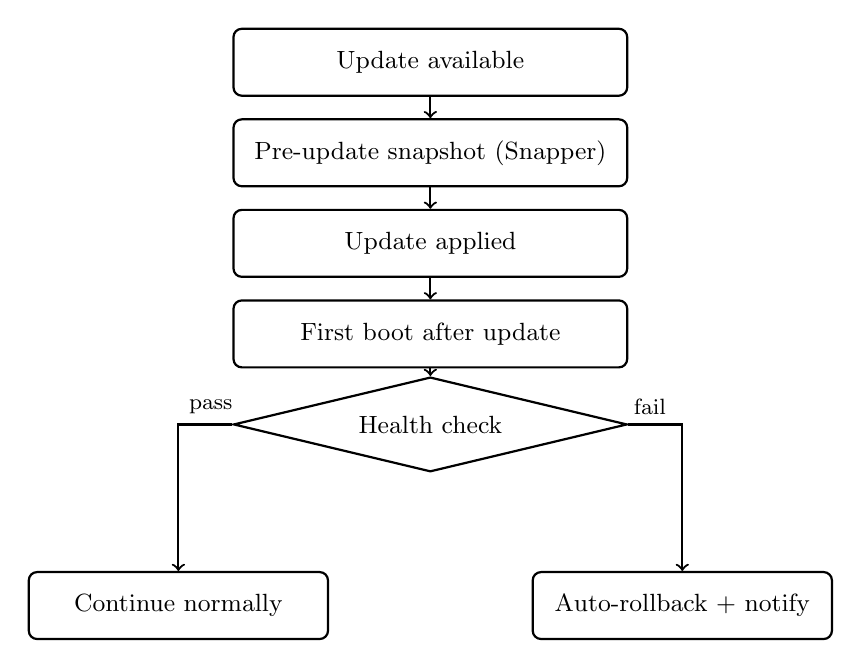
\begin{tikzpicture}[
  block/.style={
    draw, thick, rectangle, rounded corners=3pt,
    minimum width=5cm, minimum height=0.85cm,
    font=\small, align=center, inner sep=5pt
  },
  decision/.style={
    draw, thick, diamond, aspect=3,
    minimum width=5cm, minimum height=0.85cm,
    font=\small, align=center, inner sep=4pt
  },
  outcome/.style={
    draw, thick, rectangle, rounded corners=3pt,
    minimum width=3.8cm, minimum height=0.85cm,
    font=\small, align=center, inner sep=5pt
  },
  arr/.style={->, thick},
]
\def\sep{1.15}
\node[block]    (avail) at (0, 4*\sep) {Update available};
\node[block]    (snap)  at (0, 3*\sep) {Pre-update snapshot (Snapper)};
\node[block]    (apply) at (0, 2*\sep) {Update applied};
\node[block]    (boot)  at (0, \sep)   {First boot after update};
\node[decision] (check) at (0, 0)      {Health check};
\node[outcome]  (ok)    at (-3.2, -2*\sep) {Continue normally};
\node[outcome]  (fail)  at ( 3.2, -2*\sep) {Auto-rollback + notify};
\draw[arr] (avail) -- (snap);
\draw[arr] (snap)  -- (apply);
\draw[arr] (apply) -- (boot);
\draw[arr] (boot)  -- (check);
\draw[arr] (check.west) -| node[pos=0.2, above, font=\footnotesize] {pass} (ok);
\draw[arr] (check.east) -| node[pos=0.2, above, font=\footnotesize] {fail} (fail);
\end{tikzpicture}
\caption{Update flow. A Snapper snapshot is created before every update.
If the post-update health check fails, the system rolls back to the snapshot
automatically and notifies the user.}
\label{fig:update-flow}
\end{figure}

\paragraph{Btrfs and copy-on-write.}
Most widely used Linux filesystems, including \emph{ext4}, use
\emph{overwrite-in-place} semantics: when a file is modified, the old data is
replaced at the same disk location. Once overwritten, the previous version is
gone.

\emph{Btrfs}~\cite{archwiki:btrfs}
(B-Tree Filesystem) uses \emph{copy-on-write} (CoW) semantics instead. When a
file is modified, Btrfs writes the new data to a different location on disk and
updates the metadata pointer. The old version remains intact until space is
explicitly reclaimed. This has two important consequences: filesystem snapshots
become nearly free in terms of disk space (a snapshot is a set of metadata
pointers to existing blocks, not a copy of the data), and the filesystem remains
self-consistent after a crash because incomplete writes never overwrite existing
valid data.

Btrfs was merged into the Linux kernel in 2009 and has been the default
filesystem on Fedora since 2020. Its CoW architecture is the technical
foundation for this project's rollback strategy.

\paragraph{Btrfs subvolumes.}
A \emph{subvolume} is a named, independently snapshotable region of a Btrfs
filesystem. It behaves like a directory but can be mounted separately, snapshotted
independently, and assigned its own quota limits. This project uses the following
layout, consistent with the convention established by Fedora:

\begin{lstlisting}[language=bash]
@          ->  mounted at /            (system root)
@home      ->  mounted at /home        (user data)
@snapshots ->  mounted at /.snapshots
@log       ->  mounted at /var/log
@cache     ->  mounted at /var/cache
\end{lstlisting}

Keeping \texttt{/} and \texttt{/home} on separate subvolumes means a system
rollback (restoring \texttt{@} to a previous snapshot) never touches user data
in \texttt{@home}. Log and cache data are excluded from system snapshots,
preventing large log files from inflating snapshot sizes.

\paragraph{Snapper.}
\emph{Snapper}~\cite{archwiki:snapper}
is the snapshot management tool that sits on top of Btrfs. It handles creating,
listing, comparing, and restoring snapshots automatically. Snapper is configured
per subvolume: the \texttt{@} subvolume gets automatic pre/post snapshots around
package manager operations and a timeline policy for background snapshots. The
\texttt{@home} subvolume has its own independent daily snapshot schedule.

Before any update is applied, Snapper creates a tagged pre-update snapshot of
the \texttt{@} subvolume. This is a precondition for the update, not an optional
step. A matching post-update snapshot is created after the package manager
finishes, forming a before/after pair that Snapper can diff to show exactly what
changed.

\paragraph{Bootloader integration.}
The bootloader is configured to list available snapshots as boot entries. If an
update produces a system that fails to boot, the firmware presents the previous
snapshot as a selectable entry on the next start. No terminal or recovery mode
is required. On Fedora this is handled by \texttt{grub2-snapper-plugin}.

\paragraph{Post-update health check.}
On the first boot after an update, a systemd oneshot service runs a health check
before the desktop session starts. It verifies that the display system
initializes, that the network stack is reachable, that the Graph Daemon and
Event Bus start successfully, and that no systemd services have entered a failed
state. If any check fails, the service triggers an automatic rollback by setting
the pre-update snapshot as the default boot entry and rebooting. The user
receives a plain-language notification on the rolled-back system.

\paragraph{Snapshot retention.}
Snapper's retention policy for this project removes snapshots older than seven
days while always retaining the five most recent. Both values are user-adjustable
in Settings. The \texttt{@home} subvolume retains the three most recent daily
snapshots; home snapshots are a safety net for accidental file deletion, not a
system recovery mechanism.

\subsection{System Infrastructure}
\label{sec:infra}

\paragraph{systemd.}
\emph{systemd}~\cite{archwiki:systemd}
is the init system and service manager on Fedora and on
most modern Linux distributions. When the kernel finishes booting, the first
userspace process it starts is \texttt{systemd} (PID~1), which reads
\emph{unit files} describing each service, its dependencies, and its startup
environment, and starts them in dependency order. systemd also handles logging
via the \emph{journal}, socket activation, timer-based scheduling, and hardware
event management.

All custom daemons in this project are deployed as systemd service units.
systemd's unit file format provides sandboxing options that are enforced at the
kernel level without any code changes in the service: \texttt{PrivateNetwork=true}
to deny all network access, \texttt{PrivateTmp} for an isolated temporary
directory, \texttt{MemoryDenyWriteExecute} to prevent writable executable memory,
and \texttt{SystemCallFilter} to allowlist only the syscalls the service
actually needs.

\paragraph{systemd-homed.}
\emph{systemd-homed}~\cite{archwiki:homed} is a systemd component
that manages user home directories as self-contained, portable, encrypted
images. Unlike traditional Unix home directories, which are plain directories
under \texttt{/home} identified by a numeric user ID, a systemd-homed home is a
\emph{LUKS-encrypted loopback image}: a file on disk that is mounted at login
(after the encryption key is derived from the user's credentials) and unmounted
at logout. When a user is not logged in, their home directory is an opaque
encrypted file; even root cannot read its contents without the user's passphrase.

This is the technical foundation for the profile isolation system described in
Section~\ref{sec:platform}: each profile is a Linux system user with its own
systemd-homed image. When a profile is not active, its image is unmounted and
its key is discarded from memory.

\emph{LUKS} (Linux Unified Key
Setup~\cite{archwiki:luks}) is
the standard disk encryption layer on Linux, built on top of the
\texttt{dm-crypt} kernel module. It provides a standardized header format for
encrypted block devices, support for multiple key slots so that several
passphrases or key files can unlock the same volume, and memory-hard key
derivation functions that make offline brute-force attacks expensive. LUKS is
what systemd-homed uses internally to encrypt each home image.

\paragraph{Session manager and greeter.}
User sessions are managed by \emph{greetd}~\cite{greetd}, a minimal login
daemon that handles authentication and session startup. greetd is
intentionally small: it authenticates the user via PAM, launches the
configured session command on success, and exits. All policy decisions, visual
presentation, and user-facing interaction are delegated to a separate
\emph{greeter} process that communicates with greetd over a Unix socket using a
simple JSON protocol.

This clean separation between authentication daemon and login UI is why greetd
was chosen over display managers such as GDM or SDDM, which bundle both
concerns into a single process with their own GUI frameworks. The login screen
in this project is a first-party Tauri application that implements the greetd
IPC protocol: it presents the user interface, collects credentials, and passes
them to greetd for PAM verification. The Tauri greeter has access to nothing
other than the greetd socket; it runs before any user session is active, with
no access to the graph, the event bus, or any user data.

\paragraph{Package management.}
At the base level, \texttt{dnf}~\cite{dnf} handles dependency resolution,
cryptographic package signature verification, and repository management.

First-party project packages are built and distributed through the \emph{Open
Build Service} (OBS~\cite{obs}). OBS is a hosted build infrastructure
originally developed by SUSE and used by many open-source projects across
distribution families. Developers push package source files to OBS; OBS builds
the resulting RPMs in a clean Fedora chroot for every configured release target
and architecture, signs them with the project GPG key, and hosts the resulting
repository. This keeps the build pipeline reproducible and independent of the
developer's local environment.

\paragraph{Flatpak.}
Store applications are distributed as
\emph{Flatpak}~\cite{archwiki:flatpak}
packages. Flatpak is a distribution-agnostic packaging format for desktop
applications. A Flatpak bundles an application together with its specific
library dependencies into a sandboxed unit that runs isolated from the rest of
the system using Linux namespaces and \emph{bubblewrap}, with controlled access
to host resources via the \emph{XDG Desktop Portal}.

The alternative formats are \emph{Snap}, which routes all distribution through
Canonical's servers and has faced criticism for this centralization, and
\emph{AppImage}, which is a self-contained executable with no sandboxing and no
integrated update mechanism. Flatpak was chosen for its sandboxing model,
distribution neutrality, and strong support in both Fedora and the broader Linux
desktop ecosystem.

System-level components ship as native RPMs because they require tight
integration with the system: daemons must run outside any sandbox, and systemd
unit files must be installed to system paths. The Store handles both formats
transparently.

\subsection{Hardware Requirements}
\label{sec:hardware}

Three hard requirements determine the minimum supported hardware. They are not
adjustable without significant changes to the security and graphics stack and
are treated as hard constraints. In practice they exclude hardware older than
roughly 2018--2019.

\begin{table}[htbp]
\caption{Minimum hardware requirements}
\label{tab:hardware}
\begin{tabularx}{\linewidth}{lX}
\toprule
\textbf{Requirement} & \textbf{Reason} \\
\midrule
Linux kernel 6.6 or newer &
  Required for the eBPF program types used by the event monitoring system
  (Section~\ref{sec:ebpf}): \texttt{BPF\_PROG\_TYPE\_TRACEPOINT} for syscall
  attachment, \texttt{BPF\_PROG\_TYPE\_PERF\_EVENT} for process lifecycle,
  and CO-RE (Compile Once, Run Everywhere) via BTF type information for
  portable eBPF binaries. Kernel 6.6 is the LTS release that ships with
  current Fedora. \\
Vulkan-capable GPU &
  Required for hardware-accelerated compositing and for Windows compatibility
  via DXVK and vkd3d-proton. Covered automatically on AMD and Intel via Mesa;
  Nvidia requires the proprietary driver, with installer guidance provided. \\
systemd 255 or newer &
  Required for full systemd-homed portable home image functionality used by
  the profile system. \\
\bottomrule
\end{tabularx}
\end{table}

\paragraph{eBPF program types and CO-RE.}
The event monitoring system uses three eBPF program types. Tracepoint programs
attach to kernel syscall entry and exit points (\texttt{openat},
\texttt{execve}, \texttt{connect}, and others) and fire on every matching
call across all processes. Perf event programs handle process lifecycle events
including fork and exit. Ring buffer maps transfer collected events to
userspace with low overhead and without copying data through the kernel I/O
path.

All eBPF programs are compiled to eBPF bytecode at build time using the
\texttt{aya}~\cite{aya} framework and ship as pre-compiled binaries in the
system image. No compiler is required on the end-user's machine. The programs
use \emph{CO-RE} (Compile Once, Run Everywhere)~\cite{ebpf:core}, a mechanism
introduced in Linux 5.2 that uses BTF (BPF Type Format) kernel debug
information to make eBPF programs portable across kernel versions without
recompilation. Kernel 6.6 guarantees that the required BTF information is
present and that the specific tracepoint hooks this system attaches to are
stable. Kernels older than 5.8 lack ring buffer map support
entirely~\cite{ebpf:ringbuf}; kernels between 5.8 and 6.5 may work but are
not tested and not supported.

\paragraph{Vulkan.}
\emph{Vulkan}~\cite{vulkan} is a low-level graphics and
compute API by the Khronos Group, designed as the modern replacement for OpenGL.
It provides explicit control over the GPU at the cost of a more verbose API.
This project requires Vulkan for two reasons: the compositor uses Vulkan
for hardware-accelerated compositing, and the Windows compatibility layer
(Section~\ref{sec:gaming}) translates Direct3D calls to Vulkan via DXVK and
vkd3d-proton. On AMD and Intel hardware, Vulkan support is provided by
\emph{Mesa}~\cite{mesa}, the open-source graphics
driver stack included with Fedora. Nvidia hardware requires
Nvidia's proprietary driver because the open-source \texttt{nouveau} driver does
not provide Vulkan support on most hardware generations.

\paragraph{Hardware support scope.}
The design principle ``works on first boot'' requires an honest statement of
scope. It means: on supported hardware classes, the system boots, the desktop
starts, networking works, and audio works without manual configuration.

The supported hardware classes where this principle holds are mainstream x86-64
laptops and desktops with Intel or AMD CPUs released after 2018, with
integrated or discrete Intel or AMD graphics. This covers the large majority
of consumer hardware available today.

Two known categories require additional handling. Nvidia discrete GPUs require
the proprietary driver~\cite{fedora:nvidia}. RPM Fusion is configured as a
repository source in the system image; on first boot, the installer detects
Nvidia hardware and installs the proprietary driver automatically before the
user reaches the desktop. No manual repository configuration is required.
Broadcom Wi-Fi adapters, found in some Apple hardware and a smaller set of
laptops, require a proprietary driver that is not included in the Fedora
kernel~\cite{fedora:broadcom}. The same first-boot detection logic applies
where a driver package is available; hardware without a packaged driver is
documented explicitly in the compatibility list rather than discovered by
users after installation.

\subsection{Configuration Format}
\label{sec:config}

All system components and first-party applications use
\emph{TOML}~\cite{toml} (Tom's Obvious Minimal Language) as
the configuration format. TOML was designed by Tom Preston-Werner (co-founder of
GitHub) to be unambiguous and easy to edit without special tooling.

The two most common alternatives are \emph{YAML} and \emph{JSON}. YAML is
human-readable and widely used, but its indentation-sensitive syntax is a
consistent source of subtle errors: a single misaligned space changes the meaning
of the document, and certain values parse unexpectedly (bare \texttt{NO} is a boolean in YAML~1.1, not a string; YAML~1.2 fixes this, but library support for 1.2 is inconsistent in practice). JSON is unambiguous but has no comment
support and is more verbose than necessary for human-edited files.

TOML has clear, explicit syntax with no indentation sensitivity, supports inline
comments, and has an unambiguous type system: strings, integers, floats,
booleans, datetimes, arrays, and tables. Using one format consistently means a
developer who reads one configuration file can read all of them, and validation
and migration tooling only needs to be written once.

Personal settings live at
\texttt{\textasciitilde/.config/<app-id>/config.toml} and system-wide settings
at \texttt{/etc/<service-name>/config.toml}, following the
\emph{XDG Base Directory Specification}~\cite{xdg:basedir}. Some third-party applications expect other formats; a
small helper translates without moving the source of truth:

\begin{lstlisting}[language=bash]
# Export as environment variables for a legacy app
eval $(os-config-helper export \
    --toml ~/.config/myapp/config.toml --format env)

# Export as JSON for tools that require it
os-config-helper export \
    --toml ~/.config/myapp/config.toml --format json
\end{lstlisting}

The TOML file is always the authoritative source; the helper is a read-only
translation layer with no business logic of its own.

\section{Event System and Knowledge Graph}
\label{sec:event-knowledge}

\subsection{Overview}
\label{sec:event-overview}

For the Knowledge Graph to build a picture of what is happening on the machine,
something has to watch and report. The Event System is that something: it
observes activity across the entire OS and feeds a continuous stream of
structured events into the graph, without any visible effect on the user and
without requiring applications to be rewritten for this platform.

Three sources feed into it, each covering a different slice of system activity.

\begin{table}[htbp]
\caption{Event sources and their coverage}
\label{tab:event-sources}
\begin{tabularx}{\linewidth}{lXX}
\toprule
\textbf{Source} & \textbf{App cooperation} & \textbf{What it sees} \\
\midrule
Kernel monitoring (eBPF) &
  None required &
  File opens, network connections, process lifecycle \\
Wayland compositor &
  Built-in (compositor is part of this project) &
  Window focus, app open/close, clipboard operations \\
First-party app events &
  Required; apps emit events directly &
  Rich semantic actions: document saved, search performed, tab opened \\
\bottomrule
\end{tabularx}
\end{table}

The design goal is baseline coverage for every app on the system without
requiring anything from third-party developers, combined with richer semantic
data where apps support it. eBPF provides the floor; structured app events
raise the ceiling.

\subsection{Kernel Monitoring with eBPF}
\label{sec:ebpf}

\emph{eBPF} (extended Berkeley Packet Filter) is a Linux kernel subsystem that
allows small, sandboxed programs to run inside the kernel without modifying
kernel source code or loading a kernel module~\cite{ebpf:io}. The name is
historical: the original Berkeley Packet Filter from 1992 was a mechanism for
filtering network packets; the \emph{extended} version, introduced in Linux
3.18 (2014) and substantially expanded in subsequent releases, is a
general-purpose in-kernel execution environment with applications far beyond
networking.

Before eBPF, the two main approaches to system monitoring were kernel modules
and \texttt{ptrace}. A kernel module runs with full kernel privileges and no
sandboxing; a bug in a module crashes the system. \texttt{ptrace} is a syscall
that allows one process to intercept the syscalls of another, but it introduces
substantial overhead and can only observe one process at a time. eBPF solves
both problems: programs are verified by the kernel's eBPF verifier before
loading (the verifier rejects any program that could loop infinitely, access
out-of-bounds memory, or crash the kernel), run at near-native speed via JIT
compilation, and can attach to hooks covering all processes on the system
simultaneously.

An eBPF program attaches to a specific kernel hook, called a \emph{tracepoint}
or \emph{kprobe}, and is executed each time the corresponding event fires: a
file being opened (\texttt{openat} syscall), a new process being created
(\texttt{clone}/\texttt{execve}), a network connection being established, and
so on. The program runs in kernel context, collects the relevant data (file
path, process ID, return value), and passes it to a user-space daemon via a
shared \emph{ring buffer} without the overhead of standard kernel I/O paths.
The result is a read-only window into every process on the machine with overhead
typically below 2\% of CPU time under normal desktop load.

At this layer, the system knows \emph{that} a process opened a file but not
\emph{why} or what it means to the user. That is intentional: eBPF provides the
universal baseline, and higher-level sources fill in the semantics where they
are available.

\paragraph{Why aya.}
Three libraries exist for writing eBPF programs from user space:
\texttt{libbpf}~\cite{libbpf}, \texttt{BCC} (BPF Compiler Collection), and
\texttt{aya}~\cite{aya}.

\texttt{libbpf} is the reference C library maintained in the Linux kernel tree.
It is stable and widely used, but integrating it into a Rust codebase requires
C FFI (Foreign Function Interface) bindings. Every call across the Rust/C
boundary requires \texttt{unsafe} blocks that the Rust compiler cannot verify,
partially defeating the purpose of writing the daemon in Rust.

\texttt{BCC} takes a different approach: eBPF programs are written as C strings
embedded in Python or Lua and compiled at runtime by LLVM on the target machine.
This makes BCC inappropriate for a production daemon: it requires LLVM to be
present on the user's system, compilation adds startup latency of several
seconds, and the Python runtime overhead is significant for a background service.

\texttt{aya} is a Rust-native eBPF library~\cite{aya}. Both the eBPF programs
(which run inside the kernel) and the user-space daemon are written in Rust.
Programs are compiled to eBPF bytecode at build time using \texttt{cargo}, not
at runtime, so no compiler is required on the end-user's machine. The result is
a fully Rust codebase with no unsafe FFI boundaries, no runtime compilation, and
no additional system dependencies beyond what the kernel already provides.

\paragraph{Noise filtering.}
eBPF can generate thousands of events per second under normal load, most of
which carry no useful information for the Knowledge Graph. Two filters in the
normalizer reduce this before events reach the bus. Identical operations on the
same file by the same process within 100 milliseconds are collapsed into a
single event with an updated timestamp. Paths under \texttt{/proc},
\texttt{/sys}, \texttt{/dev}, \texttt{/tmp}, and shared libraries under
\texttt{/usr/lib} are discarded entirely, since they have no semantic value in
a graph of user activity.

\subsection{Event Bus}
\label{sec:event-bus}

The Event Bus is a background daemon that receives events from all sources,
validates them against the event schema, and forwards them to registered
consumers. Its only job is to move and validate data; it does not interpret or
store anything. Figure~\ref{fig:event-flow} shows the full pipeline.

\begin{figure}[htbp]
\centering
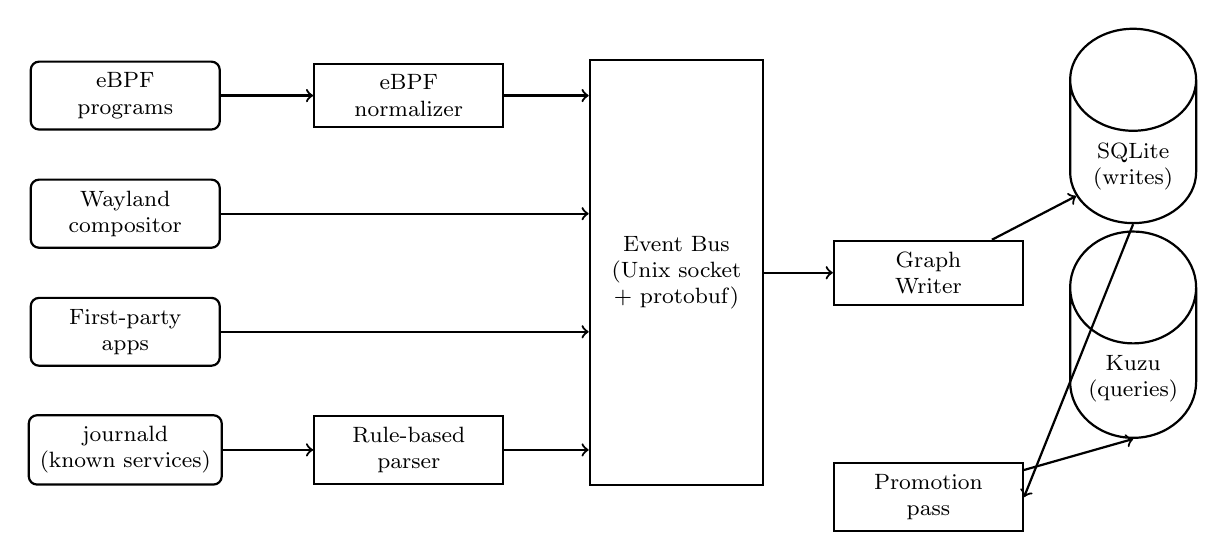
\begin{tikzpicture}[
	src/.style={
		draw, thick, rectangle, rounded corners=3pt,
		minimum width=2.4cm, minimum height=0.8cm,
		font=\footnotesize, align=center, inner sep=4pt
	},
	proc/.style={
		draw, thick, rectangle,
		minimum width=2.4cm, minimum height=0.8cm,
		font=\footnotesize, align=center, inner sep=4pt
	},
	store/.style={
		draw, thick, cylinder, shape border rotate=90,
		minimum width=1.6cm, minimum height=1.0cm,
		font=\footnotesize, align=center, inner sep=4pt
	},
	arr/.style={->, thick},
	]
	
	% Sources (x=0)
	\node[src] (ebpf)    at (0, 4.5) {eBPF\\programs};
	\node[src] (wayland) at (0, 3.0) {Wayland\\compositor};
	\node[src] (apps)    at (0, 1.5) {First-party\\apps};
	\node[src] (journal) at (0, 0.0) {journald\\(known services)};
	
	% Pre-processors (x=3.6)
	\node[proc] (norm)   at (3.6, 4.5) {eBPF\\normalizer};
	\node[proc] (parser) at (3.6, 0.0) {Rule-based\\parser};
	
	% Event Bus (x=7.0) — tall box centered at y=2.25
	\node[proc, minimum width=2.2cm, minimum height=5.4cm, text width=1.8cm]
	(bus) at (7.0, 2.25) {Event Bus\\(Unix socket\\+ protobuf)};
	
	% Graph Writer (x=10.2), SQLite (x=12.8), Kuzu (x=12.8 lower)
	\node[proc]  (gw)     at (10.2, 2.25) {Graph\\Writer};
	\node[store] (sqlite) at (12.8, 3.6)  {SQLite\\(writes)};
	\node[store] (kuzu)   at (12.8, 0.9)  {Kuzu\\(queries)};
	\node[proc]  (promo)  at (10.2, -0.6) {Promotion\\pass};
	
	% Source arrows
	\draw[arr] (ebpf)    -- (norm);
	\draw[arr] (norm)    -- (bus.west |- norm);
	\draw[arr] (wayland) -- (bus.west |- wayland);
	\draw[arr] (apps)    -- (bus.west |- apps);
	\draw[arr] (journal) -- (parser);
	\draw[arr] (parser)  -- (bus.west |- parser);
	
	% Bus -> Writer -> SQLite, SQLite -> Promotion -> Kuzu
	\draw[arr] (bus.east) -- (gw);
	\draw[arr] (gw)       -- (sqlite);
	\draw[arr] (sqlite.south) -- (promo.east);
	\draw[arr] (promo)    -- (kuzu.south);
	
\end{tikzpicture}
\caption{Event pipeline. Raw kernel events pass through the eBPF normalizer
before reaching the bus. journald output from known system services passes
through a rule-based parser. First-party app events and compositor events
arrive already structured. All sources converge on the Event Bus, which
validates and forwards to the Graph Writer Daemon. The Graph Writer writes
to SQLite at full event throughput; a background promotion pass periodically
moves semantically valuable nodes into Kuzu for graph traversal queries.}
\label{fig:event-flow}
\end{figure}

\paragraph{Event schema.}
Every event, regardless of source, shares a common envelope. The identifier
uses \emph{UUID~v7}~\cite{rfc9562}, a variant of the universally unique
identifier standard introduced in RFC~9562 (2024). Unlike UUID~v4, which is
purely random, UUID~v7 embeds a millisecond-precision Unix timestamp in the
most significant bits. This makes UUIDs generated close together sort together
lexicographically, which matters for a time-series workload: inserting events
into the graph in roughly time order avoids the random-access write pattern
that UUID~v4 would produce and improves query performance for time-range
lookups. The envelope also carries a microsecond timestamp, a type label, a
source identifier, the originating process ID, and a session reference. The
type-specific data travels as a protobuf payload inside the envelope.

\begin{lstlisting}[language=C, caption={Common event envelope (protobuf)}]
message Event {
  string id         = 1;  // UUID v7 (time-sortable)
  string type       = 2;  // "file.opened", "window.focused", etc.
  int64  timestamp  = 3;  // microseconds since epoch
  string source     = 4;  // "ebpf", "wayland", "app:<id>"
  uint32 pid        = 5;  // originating process
  string session_id = 6;  // user session reference
  bytes  payload    = 7;  // type-specific protobuf message
}
\end{lstlisting}

A \texttt{file.opened} payload carries the file path, the application name,
and the operation flags. A \texttt{window.focused} payload carries the app ID
and window title. App events use a generic structure with a category, an
action, a subject, and an optional metadata map, which allows any first-party
application to emit meaningful events without requiring a dedicated payload
type per application.

Clipboard content is never logged. The bus records that a clipboard operation
occurred and its MIME type, not the content itself.

\paragraph{D-Bus coexistence.}
The custom Event Bus handles communication between project-internal components
only. D-Bus remains in place for everything it already handles: desktop
notifications, NetworkManager, Bluetooth, session management via
\texttt{systemd-logind}, sandboxed app portals, and standard third-party
applications. The two systems run in parallel with no overlap; nothing that
communicates over D-Bus today is changed.

\subsection{Write Architecture}
\label{sec:backpressure}

The Knowledge Graph has two structurally different workloads: a high-frequency
write path that must absorb thousands of eBPF events per second without
dropping data, and a query path that must traverse multi-hop graph
relationships efficiently for AI context and user queries. These two workloads
have conflicting requirements. A database optimized for one performs poorly at
the other. The write architecture addresses this by separating the two into
dedicated stores.

\paragraph{SQLite as the write store.}
All incoming events are written to \emph{SQLite}~\cite{sqlite}, a
battle-tested embedded relational database with excellent write throughput for
append-heavy workloads. SQLite is the write store: every event from every
source lands here first, at full throughput, with no analytical overhead.

The Graph Writer Daemon maintains a ring buffer of 10,000 event slots. A
batch write to SQLite is triggered by whichever threshold is reached first:
500 milliseconds have elapsed, or 1,000 events have accumulated. Both values
are configurable. When the buffer is full, the system works through three tiers
before discarding anything. First, it checks whether an identical event (same
type, source, and subject) already exists in the buffer and updates its
timestamp rather than inserting a duplicate. If no duplicate exists, it drops
the lowest-value event in the buffer, prioritizing raw eBPF read and write
events with no app-level context. Only if neither approach frees a slot is the
incoming event discarded, which should not occur under normal operating
conditions. Drop rates per tier are exposed as metrics and monitored by the
Anomaly Detector.

Raw eBPF events are retained in SQLite for 30 days and then discarded. They
serve the anomaly detection window and nothing else; they are never promoted
to Kuzu.

\paragraph{Kuzu as the query store.}
\emph{Kuzu}~\cite{kuzu} is the query store: an embedded graph database written
in C++ with first-class Rust bindings, released under the MIT license.
Embedded means it runs inside the Graph Daemon process with no separate server
process, no network port, and no additional service to manage. Kuzu uses
\emph{Cypher}~\cite{opencypher} as its query language, which is the interface
the AI daemon, first-party applications, and the FUSE timeline daemon all use
for graph traversal.

Kuzu operates on a curated graph, not a raw event log. Raw eBPF noise never
reaches it. Only semantically valuable nodes are promoted here: \texttt{File},
\texttt{App}, \texttt{Session}, \texttt{Project}, \texttt{UserAction}, and
their relationships. This keeps the Kuzu graph clean and traversal queries
fast.

\paragraph{Promotion pipeline.}
A background promotion pass runs periodically during idle periods, reading
from SQLite and writing promoted nodes and edges to Kuzu. The pass is
incremental: it tracks a high-water mark in SQLite and processes only new
records since the last run. Promotion criteria are deterministic: \texttt{Event}
nodes that have been correlated into \texttt{UserAction} clusters, \texttt{File}
nodes that have been accessed more than once, and all \texttt{Session} and
\texttt{Project} nodes are promoted. Single-occurrence raw eBPF events that
have not been correlated are not promoted.

The two stores have different query surfaces. SQLite answers time-range
lookups over recent raw events; Kuzu answers multi-hop graph traversals over
semantic history. The Graph Daemon presents a unified query interface to all
callers; the layer boundary is an implementation detail they never see.

\begin{lstlisting}[language=SQL, caption={Example Cypher query against Kuzu: files accessed last Tuesday}]
MATCH (f:File)-[:OPENED_BY]->(a:App)
WHERE f.last_modified > datetime('2026-03-01')
RETURN f.path, a.name
ORDER BY f.last_modified DESC
\end{lstlisting}

\subsection{Knowledge Graph}
\label{sec:knowledge-graph}

\paragraph{Why a graph.}
A relational database stores relationships as foreign keys across tables. A
graph database stores them as first-class edges. The difference is felt most
when querying across multiple entity types simultaneously: finding which files
a user worked on last Tuesday, which applications touched them, and whether any
of those applications are still running requires three joins and a subquery in
SQL and a single traversal in a graph. For an operating system where
everything is connected (processes open files, files belong to projects,
projects span sessions, sessions overlap with other applications), a graph
models the domain naturally.

The write architecture that feeds the graph is described in
Section~\ref{sec:backpressure}: SQLite absorbs the high-frequency event
stream, and a promotion pipeline moves semantically valuable data into Kuzu
for graph traversal. This section describes the Kuzu graph itself: its schema,
ingestion tiers, and the data that lives in it.

\paragraph{Schema.}
Figure~\ref{fig:kg-schema} shows the core node types and their relationships.
The schema is intentionally minimal at this stage; it will grow as the system
matures. \texttt{File}, \texttt{App}, \texttt{Session}, \texttt{Project},
\texttt{Event}, and \texttt{UserAction} are the primary entities. Every raw
occurrence from the event pipeline lands in SQLite first; promotion to Kuzu
happens after correlation into higher-level nodes. \texttt{UserAction} nodes
are derived abstractions built from clusters of related events and represent
meaningful activity rather than individual syscalls.

\paragraph{Event ingestion tiers.}
Not all event sources are equal in structure or volume, and the ingestion
strategy reflects that. Three tiers operate independently. All three write
to SQLite first via the write architecture described in
Section~\ref{sec:backpressure}; promotion to Kuzu follows asynchronously.

\emph{Tier~1: structured sources.} eBPF events, compositor events, and
first-party app events arrive already typed and schema-validated. They are
written to SQLite with no intermediate processing step. This tier handles
the large majority of writes and is the only tier with hard latency
requirements.

\emph{Tier~2: rule-based parsing.} journald output from known system services
(NetworkManager, bluetoothd, systemd-logind, and others) carries useful
structured information in a line-oriented format. A rule-based parser with
per-service patterns extracts this information synchronously. No machine
learning is involved; the patterns are deterministic and fast. Unknown services
and unmatched lines are discarded rather than approximated.

\emph{Tier~3: semantic enrichment (opt-in).} For document content specifically
--- PDFs opened in the viewer, browser page titles, text file contents --- a small
local model running at idle can extract topic labels and named entities and
attach them as properties on the corresponding \texttt{File} or \texttt{Event}
node. This is explicitly opt-in, runs only during idle periods, makes no
real-time promises, and is the only tier that involves a language model.
The appropriate model class is a sub-2B parameter instruction model
(Qwen2.5-1.5B or similar) that can run on CPU without saturating it; the
workload is low-frequency enrichment of user documents, not stream processing.
The graph is fully functional without this tier enabled.
The graph is fully functional without this tier enabled.

\begin{figure}[htbp]
\centering
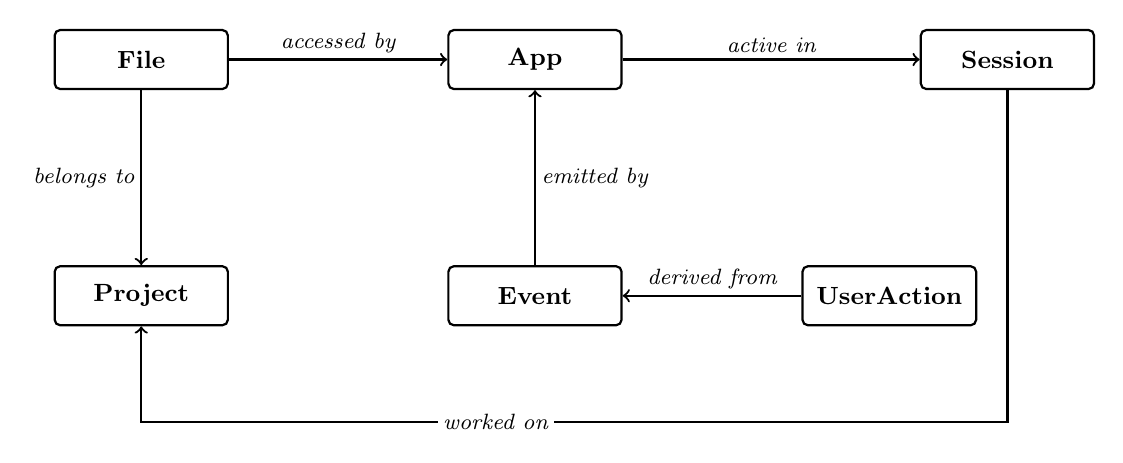
\begin{tikzpicture}[
	node/.style={
		draw, thick, rectangle, rounded corners=2pt,
		minimum width=2.2cm, minimum height=0.75cm,
		font=\small\bfseries, align=center, inner sep=5pt
	},
	edge/.style={->, thick},
	lbl/.style={font=\footnotesize\itshape, fill=white, inner sep=2pt},
	]
	
	\node[node] (file)    at (0, 4) {File};
	\node[node] (app)     at (5, 4) {App};
	\node[node] (session) at (11, 4) {Session};
	\node[node] (project) at (0, 1) {Project};
	\node[node] (event)   at (5, 1) {Event};
	\node[node] (action)  at (9.5, 1) {UserAction};
	
	\draw[edge] (file)   -- node[lbl, above] {accessed by}  (app);
	\draw[edge] (file)   -- node[lbl, left]  {belongs to}   (project);
	\draw[edge] (app)    -- node[lbl, above] {active in}    (session);
	\draw[edge] (event)  -- node[lbl, right] {emitted by}   (app);
	\draw[edge] (action) -- node[lbl, above] {derived from} (event);
	
	% Session -> Project: routed below all nodes
	\coordinate (sw) at (11, -0.6);
	\coordinate (se) at (0, -0.6);
	\draw[edge] (session.south) -- (sw) -- (se) -- (project.south);
	\node[lbl] at (4.5, -0.6) {worked on};
	
\end{tikzpicture}
\caption{Knowledge Graph core schema. Nodes represent entities; edges
represent relationships. \texttt{Event} nodes are the lowest-level entries,
created directly from the event pipeline. \texttt{UserAction} nodes are
derived abstractions built from clusters of raw events. A \texttt{File} can
belong to multiple \texttt{Project} nodes simultaneously; membership is an
edge, not a property of the file.}
\label{fig:kg-schema}
\end{figure}

\subsection{Project System}
\label{sec:projects}

A project is not a folder. It is a named context node in the Knowledge Graph
that groups related files, sessions, and activity across time and application
boundaries. The grouping is expressed as typed edges; a file does not carry a
project property, it participates in a \texttt{PART\_OF} relationship. This
means a file can belong to multiple projects simultaneously, and project
membership can be established, changed, or removed without touching the file
itself.

\paragraph{Philosophy: emergent, not prescribed.}
Projects are designed to arise from observed behavior and be confirmed by the
user, not to be created upfront and maintained manually. The graph accumulates
enough signal to infer that a coherent context exists; the user names and
confirms it. Both paths are available: explicit creation is supported for users
who prefer structure from the start, but it is not required.

\paragraph{The \texttt{.project} file.}
Every project can optionally carry a \texttt{.project} file at its root
directory. This is a TOML file that acts as the authoritative configuration for
that project and is the primary structured data source the Graph Daemon uses
when building the \texttt{Project} node. It is designed to be committed
alongside source code: a developer who clones a repository gets the project
context with it.

\begin{lstlisting}[language=bash, caption={Example .project file}]
[project]
name        = "CoffeeShop"
description = "Wii U homebrew mod manager"
status      = "active"   # active | paused | archived
created     = 2025-11-01
due         = 2026-06-01 # optional

[paths]
root    = "~/Repositories/coffeeshop"
include = [
    "~/Documents/coffeeshop-notes",
    "~/Downloads/wiiu-sdk-reference.pdf",
]
exclude = ["target/", "*.log"]

[git]
remote         = "https://github.com/timkicker/coffeeshop"
default_branch = "main"

[accounts]
github = "timkicker"

[links]
docs   = "https://wiiu.hacks.guide"
issues = "https://github.com/timkicker/coffeeshop/issues"

[tags]
values = ["cpp", "wiiu", "homebrew"]

[appearance]
accent_color = "#6aaa64"  # optional; overrides shell accent when focused

[focus]
suppress_notifications_from = ["steam", "discord"]

[modules]
active_when_focused = ["com.example.rust-waypointer"]

[ai]
context_scope = "project"  # minimal | project | time-scoped

[collaboration]
# Planned for a future release. The data model supports shared projects
# from the start; this field is reserved and currently ignored.
enabled = false
\end{lstlisting}

The \texttt{.project} file is the source of truth; the Graph Daemon reads it
at session start and whenever it changes on disk. Projects without a
\texttt{.project} file are fully supported: the node exists in the graph and
all features work, but configuration defaults apply and the project cannot be
distributed as a template.

\paragraph{Project node properties.}
The \texttt{Project} node in the graph carries the following properties, sourced
from the \texttt{.project} file where present and inferred or defaulted otherwise:
name, description, status, root path, creation timestamp, optional due date, tags,
and an accent color. The status field drives visibility across the system:
\texttt{active} projects appear prominently in Waypointer, the File Manager
sidebar, and AI context suggestions; \texttt{paused} projects are searchable
but not proactively surfaced; \texttt{archived} projects are read-only in the
graph and only reachable via explicit search. Archiving is a transition, not a
deletion: graph data is retained under the normal retention policy.

\paragraph{File membership and the \texttt{PART\_OF} edge.}
A file becomes part of a project through one of four mechanisms, in decreasing
order of specificity. First, explicit declaration in the \texttt{[paths]} block
of the \texttt{.project} file: any file under a declared include path is a
member. Second, rootdir heuristic: any file under the project root directory
is a candidate member, confirmed once the user has acknowledged the project.
Third, co-occurrence clustering: files that consistently appear together in the
same sessions, accessed by the same applications and terminal working directories,
are grouped as project candidates by a background inference pass. Fourth, manual
assignment via the File Manager or Waypointer: the user explicitly adds a file
to a project, which writes a \texttt{PART\_OF} edge directly.

A file can carry \texttt{PART\_OF} edges to multiple projects simultaneously.
The graph enforces no uniqueness constraint on this relationship.

\paragraph{Project-scoped AI context.}
When the AI access level is set to project-scoped (Level~2, described in
Section~\ref{sec:ai}), the \texttt{.project} file serves as the context seed
for the AI daemon. Name, description, tags, linked accounts, and recent
project activity from the graph are included in the context window before the
user's query. Waypointer surfaces project-specific quick actions when a project
is active: recent files, last commit message, open issues URL, and time spent
this week. These are graph queries, not hardcoded integrations.

\paragraph{Git integration.}
The presence of a \texttt{.git} directory in the project root is treated as a
strong project signal: the directory is automatically proposed as a project
root if no \texttt{.project} file exists. The current branch name is attached
as a property on the active \texttt{Session} node, providing context for
queries like ``what was I working on during the refactor branch last week.''
The \texttt{[git]} block in the \texttt{.project} file links the remote and
default branch for use in Waypointer quick actions and AI context.

Full git integration, covering commits as graph nodes, branch switches as
session context events, and pull request status as linked resources, is
planned for a subsequent release. The graph schema includes \texttt{Commit}
and \texttt{Branch} node types from the start so that this integration does
not require a schema migration when it arrives.

\paragraph{Project-aware system integrations.}
Projects are a cross-cutting concept and several system components integrate
with them directly. These integrations are described in detail in the
sections covering each component; the connections are summarized here for
reference.

The \emph{Focus Mode} (Section~\ref{sec:desktop}) is activated when the user
switches to a project context. It coordinates the shell accent color, Waypointer
search scope, File Manager root, terminal working directory, and notification
priority rules simultaneously.

The \emph{Health Daemon} (Section~\ref{sec:health}) tracks active focus time
per project from session data. This enables queries about work distribution
across projects and provides the signal for wellbeing observations such as
sustained single-project concentration over extended periods.

The \emph{Companion App} (Section~\ref{sec:companion}) uses the active project
as the Handoff context: switching away from the desktop surfaces the project's
linked resources, recent files, and notes on the phone.

The \emph{Module System} (Section~\ref{sec:modules}) supports the
\texttt{active\_when\_focused} manifest field, which activates a module only
when a specific project is in focus. A Rust-specific Waypointer provider that
surfaces \texttt{cargo} commands is the canonical example: it runs only when
the focused project carries the \texttt{rust} tag.

The \emph{Audit Log} (Section~\ref{sec:audit-log}) supports project-scoped
export: all activity records associated with a project within a specified date
range can be exported as a structured report. This is useful for time tracking,
client billing, and project handover.

\emph{Signed Profile Packages} (Section~\ref{sec:profiles}) can bundle
\texttt{.project} template files. An organization deploying a work profile
can pre-configure project structure, required accounts, AI scope restrictions,
and notification rules as part of the profile installation.

\paragraph{Automatic project inference.}
Project nodes in the graph are created explicitly when the user names a
project or a \texttt{.project} file is detected, but the graph also accumulates
enough signal to infer project membership without either. Files that
consistently appear together in the same sessions, terminal working directories
that recur alongside a fixed set of applications, and browser tabs that
co-occur with specific local files are all indicators that a coherent project
exists even without a name. A background inference pass groups these
co-occurrence clusters into candidate project nodes and presents them to the
user as suggestions rather than applying them automatically. The user can
confirm, rename, or dismiss each suggestion. Automatic inference is opt-in
and runs locally.

\subsection{Retention Policy}
\label{sec:retention}

The graph accumulates data indefinitely if left unchecked, which creates two
problems: storage grows, and the privacy surface area expands. The retention
policy defines how long data lives, with user control at every tier.

\begin{table}[htbp]
\caption{Knowledge Graph retention tiers}
\label{tab:retention}
\begin{tabularx}{\linewidth}{llX}
\toprule
\textbf{Tier} & \textbf{Default} & \textbf{Content} \\
\midrule
Raw eBPF events (SQLite) &
  30 days &
  High-volume, low-semantic-value syscall events. Retained for the
  anomaly detection window; never promoted to Kuzu and discarded
  after expiry. \\
Semantic nodes (Kuzu) &
  12 months rolling &
  File, App, Session, and NetworkConnection nodes promoted from SQLite.
  This is where AI query value lives. Nodes past the window
  are summarized rather than deleted. \\
Pinned nodes (Kuzu) &
  Permanent &
  Nodes explicitly marked by the user, active Project nodes, and nodes
  recently referenced in AI queries. Only manual deletion removes these. \\
\bottomrule
\end{tabularx}
\end{table}

\paragraph{Summarization.}
Hard deletion of aged nodes loses information abruptly. Instead, nodes past
the retention window are compacted into summary nodes that retain aggregate
statistics (access count, primary application, active period) while discarding
the individual event edges. The node still exists in the graph and AI queries
still find it; the granularity is reduced but the semantic content is
preserved. Summarization is triggered by access frequency rather than age: a
node that has not been queried in six months is a candidate regardless of when
it was created, while a node from two years ago that is queried regularly
remains granular. A background daemon identifies candidates nightly and
processes them during idle periods.

\paragraph{User controls.}
Settings exposes the retention window per tier with documented minimums, a
manual summarize-now option for specific time ranges, node and subgraph
deletion, full graph export for data portability, and storage usage broken down
by tier and time range. In managed deployments, administrators can set a
minimum retention for compliance-relevant audit events in a separate audit log,
but they cannot shorten the user's configured retention window for personal
graph data.

\subsection{Temporal Filesystem View}
\label{sec:temporal-fs}

The Knowledge Graph contains a complete record of which files were accessed,
created, and modified, when, and by which application. This makes it possible
to answer queries like ``show me everything I worked on last Tuesday'' without
relying on file modification timestamps, which applications regularly reset, or
on search indices, which do not capture access history.

The temporal filesystem view exposes this as a navigable virtual directory tree
via a \emph{FUSE} (Filesystem in Userspace) mount. FUSE is a Linux kernel
mechanism that allows a userspace process to implement a filesystem: the kernel
forwards directory listing and file open calls to the FUSE daemon, which
answers them from its own data source rather than from disk. The temporal view
mounts at \texttt{\textasciitilde/.timeline/} and is populated on demand by a
small daemon that translates directory traversal into Graph Daemon queries.

A path like \texttt{\textasciitilde/.timeline/2026-03-04/} lists all files the
user touched on that date, grouped by project where the graph has enough
context to determine project membership. The project grouping is deterministic
when a \texttt{.project} file is present and heuristic otherwise. Opening a
file through this path opens the actual file at its real location; the timeline
view is an index, not a copy. No additional storage is used.

\begin{lstlisting}[language=bash, caption={Temporal filesystem view examples}]
# List files worked on a specific date
ls ~/.timeline/2026-03-04/

# Browse by project across all time
ls ~/.timeline/projects/CoffeeShop/

# Files touched in the last week, grouped by project
ls ~/.timeline/last-7-days/

# Open a file as it appears in the timeline (opens real file)
xdg-open ~/.timeline/2026-03-04/CoffeeShop/report-draft.md
\end{lstlisting}

The FUSE daemon holds no persistent state of its own; every listing is a live
graph query. The mount is available only while the user session is active and
the Graph Daemon is running. It is read-only: files cannot be created, renamed,
or deleted through the timeline path.

A natural extension of the temporal view is causal chain visualization:
because the graph records not only which files were accessed but the sequence
and application context of those accesses, it is possible to reconstruct the
workflow that produced a given output. A query asking ``what did I do to produce
this file?'' can trace the chain of files opened, commands run, and applications
active in the session where the file was last modified. This is planned for a
subsequent release, built on the same FUSE and graph infrastructure described
here.

\section{AI Layer}
\label{sec:ai}

\subsection{Overview}
\label{sec:ai-overview}

The AI layer sits on top of the Knowledge Graph and provides both the user and
the system with access to an AI model that has structured context about what is
happening on the machine. It is not a chatbot grafted onto an existing OS; it
is an interface that can query the graph, invoke application capabilities
through a standardized protocol, and optionally act autonomously when the user
explicitly enables that.

The AI layer is not the primary reason this system exists. The desktop, the
permission system, the profile isolation, and the store all stand on their own.
AI is an enhancement that becomes more useful as the Knowledge Graph fills in
over time, and users who want none of it can disable it completely without
losing any other functionality.

Three principles govern the design of this layer.

\paragraph{Query-first.}
The AI responds when asked. Nothing happens in the background without an
explicit trigger. Autonomous features exist but are separate opt-ins, not
defaults that the user has to find and disable.

\paragraph{Provider-agnostic.}
The system does not care whether the model runs locally or in the cloud.
Every provider implements the same interface; the rest of the codebase never
speaks to a specific backend. The user decides what runs where, including
routing sensitive requests to a local model only.

\paragraph{Opt-out at any point.}
The entire layer can be disabled in Settings under AI. When disabled, no local
model runs, no graph queries originate from the AI layer, Waypointer falls back
to standard search, and no MCP servers are active. The setting is not hidden
five menus deep.

\subsection{Cold-Start Behavior}
\label{sec:ai-coldstart}

The Knowledge Graph is empty on a fresh install. An AI feature that promises
contextual awareness but has nothing in the graph yet is worse than no feature
at all: it creates an expectation and immediately fails to meet it. The system
handles this with straightforward communication rather than by faking
usefulness.

During onboarding, AI features are presented with an honest explanation of
what to expect: the assistant learns context gradually as the system is used,
starts with nothing, and becomes more useful over days and weeks. There are no
demo interactions, no placeholder context, and no fabricated examples of what
it will eventually be able to do.

At onboarding the user can optionally seed the graph with existing data from
their current system: browser history, calendar events, and documents. This is
presented as a trade-off, not a recommendation. Each source can be imported
independently, so someone who is comfortable sharing their calendar but not
their browsing history can import only the former. Importing gives the AI
immediately useful context without a multi-week waiting period.

The AI assistant does not surface proactively until a threshold is met: seven
days of usage or a completed manual import. Before that threshold the feature
is accessible but does not advertise itself. The non-AI parts of the system are
functional and complete from the first boot, so there is no gap in usefulness
during this period.

\subsection{Provider Abstraction}
\label{sec:ai-providers}

Different AI providers have different APIs, different latency profiles, and
significantly different privacy implications. Sending the contents of a private
file to a cloud API is appropriate in some contexts and completely unacceptable
in others. The system needs to handle both without the rest of the codebase
caring which provider is active.

The solution is a Rust trait that every AI backend implements. The AI layer
constructs a \texttt{CompletionRequest}, passes it to whichever provider is
configured, and receives a \texttt{CompletionResponse}. No provider-specific
code is visible outside the provider module. The \texttt{\#[async\_trait]}
macro~\cite{async-trait} is a Rust community crate that enables async methods
in traits, which the stable Rust compiler does not yet support natively; it
desugars the async methods into an equivalent form that compiles correctly.

\begin{lstlisting}[language=Rust, caption={AI provider trait}]
#[async_trait]
pub trait AiProvider: Send + Sync {
    async fn complete(
        &self,
        request: CompletionRequest,
    ) -> Result<CompletionResponse>;
    async fn available(&self) -> bool;
    fn name(&self) -> &str;
}
\end{lstlisting}

Figure~\ref{fig:providers} shows how the AI layer relates to the available
backends.

\begin{figure}[htbp]
\centering
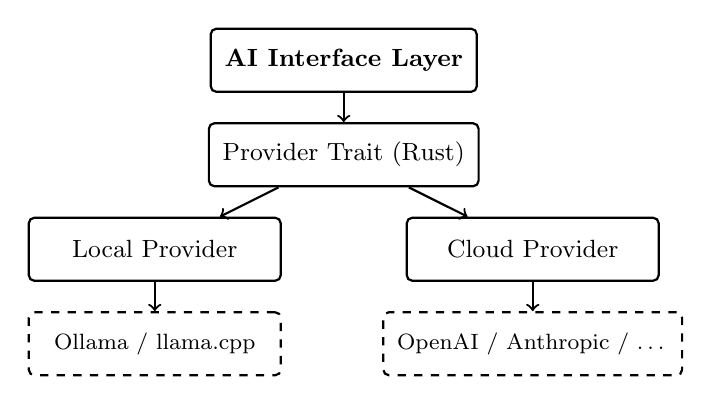
\begin{tikzpicture}[
  box/.style={
    draw, thick, rectangle, rounded corners=2pt,
    minimum width=3.2cm, minimum height=0.8cm,
    font=\small, align=center, inner sep=5pt
  },
  arr/.style={->, thick},
]

\node[box] (ail)   at (0, 3.2) {\textbf{AI Interface Layer}};
\node[box] (trait) at (0, 2.0) {Provider Trait (Rust)};
\node[box] (local) at (-2.4, 0.8) {Local Provider};
\node[box] (cloud) at ( 2.4, 0.8) {Cloud Provider};
\node[box, dashed] (lm)  at (-2.4, -0.4) {\footnotesize Ollama / llama.cpp};
\node[box, dashed] (api) at ( 2.4, -0.4) {\footnotesize OpenAI / Anthropic / \ldots};

\draw[arr] (ail)   -- (trait);
\draw[arr] (trait) -- (local);
\draw[arr] (trait) -- (cloud);
\draw[arr] (local) -- (lm);
\draw[arr] (cloud) -- (api);

\end{tikzpicture}
\caption{Provider abstraction. The AI layer speaks only to the trait; the
concrete backend is a configuration choice. Local and cloud providers are
interchangeable from the perspective of anything above the trait boundary.}
\label{fig:providers}
\end{figure}

\paragraph{Local providers.}
A local provider runs an AI model entirely on the user's machine. No data
leaves the device. The two primary options are \emph{Ollama}~\cite{ollama}
and \emph{llama.cpp}~\cite{llamacpp}.

\emph{llama.cpp} is a C++ inference engine for running large language models
on consumer hardware, originally developed by Georgi Gerganov in 2023. It
achieves viability on consumer hardware through \emph{quantization}: a
technique that reduces the numerical precision of a model's weight values
(for example from 32-bit floats to 4-bit integers), shrinking both the memory
footprint and computation cost at a modest quality trade-off~\cite{llamacpp:quant}.
A 7-billion parameter model that would require roughly 28~GB of RAM at full
32-bit precision runs in approximately 4~GB after 4-bit quantization, which
falls within the RAM budget of a typical consumer laptop. llama.cpp exposes
an HTTP API compatible with the OpenAI request format, so any client written
for the OpenAI API works against a local llama.cpp instance by changing the
base URL.

\emph{Ollama} wraps llama.cpp and other backends in a higher-level tool that
adds model management (download, version tracking, storage), a simpler CLI,
and a REST API. For most users, Ollama is the practical entry point. llama.cpp
is available as a direct option for cases where fine-grained control over
quantization levels and inference parameters is needed.

Both are supported as local provider backends. The specific model is a user
configuration choice. As of 2025, models in the 7B--13B parameter range with
4-bit quantization offer the best balance of quality, memory footprint, and
inference speed on consumer hardware without a dedicated GPU.

\paragraph{Cloud providers.}
Cloud providers send the request to a remote API over HTTPS and return the
response. The system ships with built-in support for the
OpenAI~\cite{openai:api} and Anthropic~\cite{anthropic:api} APIs, both of
which follow similar request/response formats. Additional providers can be
added by implementing the provider trait; the interface is intentionally
minimal. API keys are stored in the system keyring (not in a config file) and
are never written to the Knowledge Graph.

\paragraph{Routing policy.}
Multiple providers can be active simultaneously under a routing policy the
user configures in TOML. The baseline: use the local provider if one is
configured and available; fall back to cloud if the local model is unavailable
or if the request exceeds the local model's context window. Additional rules
can be layered on top: route all code-related requests to a specific provider;
prevent any request that includes personal file contents or graph data from
leaving the machine; route requests originating from a specific application to
a designated provider. Rules are evaluated in order; the first match wins.

\subsection{MCP Integration}
\label{sec:mcp}

\emph{MCP} (Model Context Protocol) is an open protocol published by Anthropic
in November 2024 that standardizes how AI models interact with external tools
and data sources~\cite{mcp:spec}. The core idea is a client/server split: the
AI model talks to an \emph{MCP client}, which in turn dispatches to one or more
\emph{MCP servers}. Each server exposes a list of \emph{tools} (functions the
AI can call) and \emph{resources} (data the AI can read). The protocol runs
over JSON-RPC~2.0~\cite{jsonrpc2}, a lightweight remote procedure call format,
typically over a Unix socket or stdio pipe for local servers and over HTTP/SSE
for remote ones.

The key property of MCP is that the AI model does not need to know anything
about the application it is talking to. A model that has never seen this OS
can still call \texttt{list\_directory} on the file manager MCP server,
because the tool definition (name, parameters, description) is discovered at
runtime. This makes MCP servers independently deployable and the AI layer
application-agnostic.

In this system, first-party applications expose MCP servers as part of their
standard implementation via the \emph{os-sdk} boilerplate described in
Section~\ref{sec:overview}: the file manager exposes \texttt{list\_directory},
\texttt{open\_file}, and \texttt{move\_file}; the terminal exposes
\texttt{run\_command} and \texttt{get\_output}; the Knowledge Graph exposes a
query interface. The AI can coordinate across multiple applications in a single
interaction by calling their respective servers in sequence.
Figure~\ref{fig:mcp} shows the topology.

\begin{figure}[htbp]
	\centering
	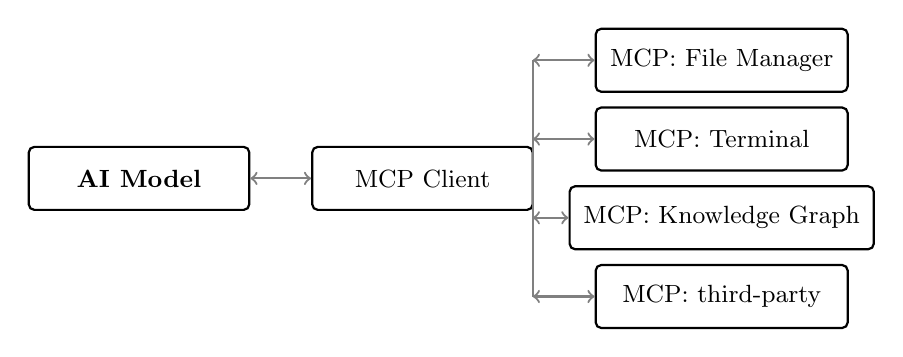
\begin{tikzpicture}[
		box/.style={
			draw, thick, rectangle, rounded corners=2pt,
			minimum width=2.8cm, minimum height=0.8cm,
			font=\small, align=center, inner sep=5pt
		},
		srv/.style={
			draw, thick, rectangle, rounded corners=2pt,
			minimum width=3.2cm, minimum height=0.8cm,
			font=\small, align=center, inner sep=5pt
		},
		arr/.style={<->, thick, gray},
		]
		
		\node[box] (model)  at (0, 0) {\textbf{AI Model}};
		\node[box] (client) at (3.6, 0) {MCP Client};
		
		\node[srv] (fm)   at (7.4,  1.5) {MCP: File Manager};
		\node[srv] (term) at (7.4,  0.5) {MCP: Terminal};
		\node[srv] (kg)   at (7.4, -0.5) {MCP: Knowledge Graph};
		\node[srv] (ext)  at (7.4, -1.5) {MCP: third-party};
		
		\coordinate (mid) at (5.0, 0);
		
		\draw[arr] (model) -- (client);
		\draw[thick, gray] (client.east) -- (mid);
		\draw[thick, gray] (mid |- fm.west)  -- (mid |- ext.west);
		\draw[arr] (mid |- fm.west)   -- (fm.west);
		\draw[arr] (mid |- term.west) -- (term.west);
		\draw[arr] (mid |- kg.west)   -- (kg.west);
		\draw[arr] (mid |- ext.west)  -- (ext.west);
		
	\end{tikzpicture}

\caption{MCP topology. The AI model communicates through a single MCP client
that dispatches to individual application servers. Third-party applications
from the Store can ship their own MCP servers, subject to the permission model
described in Section~\ref{sec:mcp-permissions}.}
\label{fig:mcp}
\end{figure}

CLI tools do not need MCP servers. If a tool has a \texttt{-{}-help} flag and
produces sensible output, the AI can invoke it as a subprocess and read
\texttt{stdout}. MCP is reserved for GUI applications and stateful interfaces
where a subprocess call is insufficient.

\subsection{Interaction Model}
\label{sec:ai-interaction}

\paragraph{Query-based (default).}
The user asks a question, the AI responds. No background activity occurs
without an explicit trigger. The AI has access to the Knowledge Graph and
whatever MCP servers are permitted under the current configuration. Typical
interactions include querying session history, finding files related to a
project, correlating system events with observed behaviour, and composing
multi-step actions across applications.

When a question is asked, the AI layer translates the natural language input
into a Cypher query, executes it against the Knowledge Graph via the Graph
Daemon, and passes the structured results to the model as context. Relative
time expressions are resolved to absolute UTC timestamps before the generation
step, so the model always operates on concrete values rather than ambiguous
phrases. The Cypher generation and the result formatting are two separate model
calls, since combining them causes the model to bias the query toward a
desired-sounding answer rather than accurately querying the schema.

The query validator sits between generation and execution: it checks that the
generated Cypher uses only known node types and relations, contains no write
operations, and includes a \texttt{LIMIT} clause. If validation fails, the
error is fed back for a retry; after two failed attempts the user is told the
question could not be answered, with no silent fallback.

\paragraph{Autonomous agent (explicit opt-in).}
A background agent that observes the event stream and acts proactively is
available as an opt-in capability. It is not enabled by default and each
autonomous behaviour is a separate toggle: suggesting related files when a
document is opened is independent of automatically tagging new files by
project. The agent uses the same provider abstraction and MCP layer as the
query interface; the difference is that it initiates actions rather than
responding to them.

\subsection{Project Context}
\label{sec:ai-project-context}

When a project is active in Focus Mode (Section~\ref{sec:focus-mode}), the AI
layer adjusts its behavior to match. This happens automatically when Focus Mode
activates and is reversed when it deactivates; no separate AI configuration is
required.

\paragraph{Context seed.}
The \texttt{.project} file (Section~\ref{sec:projects}) is loaded as a
structured context seed at the start of every AI query while a project is
focused. The model receives the project name, description, tags, linked
accounts, relevant links, and a summary of recent project activity from the
graph before processing the user's question. This is the minimum context
needed for the AI to give useful answers without the user having to re-explain
their situation every time.

\paragraph{Graph scope.}
If the project's \texttt{[ai]} block declares
\texttt{context\_scope = "project"}, the Graph Daemon restricts the AI
daemon's traversal to nodes carrying a \texttt{PART\_OF} edge to the active
project. The AI sees a narrower but more relevant slice of the graph: recent
project files, sessions where the project was active, applications used in
those sessions, and notifications received during focused work. Nodes outside
the project are not visible to the model for the duration of the focused
session.

This is Access Level~2 from the table in Section~\ref{sec:ai-security}, applied
automatically by Focus Mode rather than requiring the user to configure it
manually per session.

\paragraph{Waypointer integration.}
Inside Waypointer's AI mode (Tab), queries are answered with project context
active. Asking ``which files did I touch yesterday?'' returns results filtered
to the project rather than the full graph. Project-specific quick actions ---
recent files, last commit message, open issues link, focus time this week ---
are derived from live graph queries against the active \texttt{Project} node
and its edges, not from cached or hardcoded data.

\subsection{MCP Permission Model}
\label{sec:mcp-permissions}

MCP servers are the interface through which the AI acts on applications.
The permission model distinguishes between reading information, which the AI
can do by default within the user's configured AI permission level, and
modifying state, which requires explicit per-session authorization.

\begin{table}[htbp]
\caption{Read-only MCP servers (permitted by default)}
\label{tab:mcp-read}
\begin{tabularx}{\linewidth}{lX}
\toprule
\textbf{Server} & \textbf{Exposes} \\
\midrule
File Manager   & Directory listings, file metadata \\
Calendar       & Upcoming and past events \\
Browser        & History and open tabs (no passwords, no form data) \\
System Monitor & Process list and resource usage \\
Notes          & Note titles and content \\
\bottomrule
\end{tabularx}
\end{table}

Reading to answer a question is what the user expects when they ask the AI
something. Answering ``what meetings do I have today?'' without a confirmation
dialog is the correct behaviour. Reading does not change state, and the AI
permission level configured in Settings still gates what data each server
exposes regardless of this default.

\begin{table}[htbp]
\caption{Write and action MCP servers (per-session authorization required)}
\label{tab:mcp-write}
\begin{tabularx}{\linewidth}{lX}
\toprule
\textbf{Server} & \textbf{Can do} \\
\midrule
Terminal     & Execute shell commands \\
File Manager & Create, move, rename, delete files \\
Calendar     & Create and modify events \\
Email        & Compose and send messages \\
Store        & Install and remove packages \\
\bottomrule
\end{tabularx}
\end{table}

Authorization is granted once per session and covers the scope the user
specifies: approving file management does not imply approval for email. It
expires at session end and is not persisted. Within an authorized scope, a
separate hardcoded list of actions always requires explicit confirmation
regardless of session permissions, because their consequences are irreversible
or high-impact: permanent file deletion, sending any external message,
installing or removing system packages, modifying system configuration outside
\texttt{\textasciitilde/.config}, any network request to a host outside the
application's declared permissions, and running commands with elevated
privileges. This list is not configurable.

Third-party MCP servers shipped by Store applications are always treated as
action-requiring by default. A community server that claims to be read-only
receives the same treatment until it carries a verified security audit covering
its MCP implementation.

\subsection{System Explanation Mode}
\label{sec:ai-explain}

A running operating system is largely opaque to its user. Background processes
run, network connections open and close, disk activity spikes, and the user
has no practical way to understand what is happening without opening a terminal
and running several diagnostic commands. This is a gap this system is
positioned to close, because it already has the data.

The AI daemon can answer the question \emph{``What is my computer doing right
now?''} by querying the live event stream and the Knowledge Graph simultaneously.
The event stream provides the current moment: which processes are active, what
they are reading or writing, which network connections are open, what the CPU
and memory usage is and which process owns it. The Knowledge Graph provides
context: whether this activity is normal for this time of day on this machine,
which project the files being accessed belong to, whether this process has
behaved unusually in the past.

The result is a dynamically generated plain-language summary, not a set of
predefined status strings. A typical response might note that the package
manager is fetching updates in the background, that a first-party application
is indexing a recently imported folder, and that network activity is within the
normal range for this time of day. If something is unusual, the summary says
so: a process accessing node types it has never previously accessed, or a
network connection to a destination outside the application's declared
permissions, is flagged in the same natural language response rather than
silently logged.

The explanation mode is available on demand via the AI query interface and as
a persistent ambient view in System Monitor. It does not run continuously in
the background; it is a query like any other, executed when the user asks.
Everything it uses is local: the event stream and the Knowledge Graph never
leave the machine, and the model generating the summary runs locally unless
the user has configured a cloud provider. The output can be shared by the user
if they choose, but nothing is reported automatically.

\section{Desktop Environment and Design Language}
\label{sec:desktop}

The desktop environment is the most visible part of the system and the primary
differentiator for users switching from other platforms. The goal is a fast,
coherent desktop that does not feel like a collection of independent projects
assembled by different teams in different decades. The stack reflects this:
performance-critical and system-close code is Rust, everything visual is
TypeScript with Tailwind CSS, and the two halves communicate over well-defined
interfaces that neither side reaches past.

\subsection{Architecture and IPC}
\label{sec:desktop-ipc}

Three communication channels connect the compositor core to the shell and its
frontend, each carrying a different class of data.

\begin{figure}[htbp]
\centering
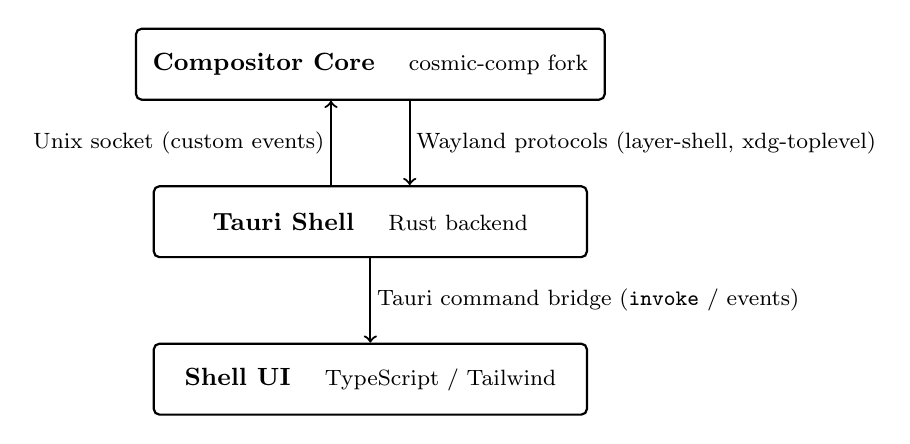
\begin{tikzpicture}[
	box/.style={
		draw, thick, rectangle, rounded corners=2pt,
		minimum width=5.5cm, minimum height=0.9cm,
		font=\small, align=center, inner sep=6pt
	},
	arr/.style={->, thick},
	lbl/.style={font=\footnotesize, fill=white, inner sep=2pt, align=center},
	]
	
	\node[box] (smithay) at (0, 4.0) {\textbf{Compositor Core} \quad {\footnotesize cosmic-comp fork}};
	\node[box] (tauri)   at (0, 2.0) {\textbf{Tauri Shell} \quad {\footnotesize Rust backend}};
	\node[box] (ui)      at (0, 0.0) {\textbf{Shell UI} \quad {\footnotesize TypeScript / Tailwind}};
	
	\draw[arr] ([xshift= 0.5cm]smithay.south) -- ([xshift= 0.5cm]tauri.north)
	node[lbl, right, midway] {Wayland protocols (layer-shell, xdg-toplevel)};
	\draw[arr] ([xshift=-0.5cm]tauri.north) -- ([xshift=-0.5cm]smithay.south)
	node[lbl, left, midway] {Unix socket (custom events)};
	
	\draw[arr] (tauri.south) -- (ui.north)
	node[lbl, right, midway] {Tauri command bridge (\texttt{invoke} / events)};
	
\end{tikzpicture}
\caption{Shell IPC architecture. Wayland protocols carry window management data
(open windows, focus, workspace state). The Unix socket carries system-specific
events with no Wayland equivalent: theme updates, module lifecycle events,
graph notifications. The Tauri command bridge connects the Rust backend to the
TypeScript frontend within the shell process.}
\label{fig:shell-ipc}
\end{figure}

Wayland protocol extensions are the correct channel for anything the Wayland
ecosystem has standardized. The Unix socket exists for everything that does not
have a protocol equivalent and where a custom solution is both simpler and more
direct. Messages on the socket use JSON during development, with migration to
protobuf planned once the schema stabilizes.

Within the Tauri shell, the Rust backend and TypeScript frontend communicate
through Tauri's typed command system: the frontend calls Rust via
\texttt{invoke()}, Rust pushes events to the frontend via Tauri's event
emitter. No ad-hoc serialization; the bridge handles it.

\subsection{Compositor and Window Manager}
\label{sec:compositor}

The Wayland compositor is a fork of \emph{cosmic-comp}~\cite{cosmic:comp},
as described in Section~\ref{sec:compositor-intro}. This section covers what
that means in practice for window management and the shell boundary.

The fork retains the full window management engine from cosmic-comp: floating
and tiling layouts switchable per workspace independently, focus rules,
workspace management, and all the low-level Wayland plumbing that cosmic-comp
inherits from \emph{Smithay}~\cite{smithay}.

\emph{DRM/KMS} (Direct Rendering Manager / Kernel Mode Setting) is the Linux
kernel subsystem responsible for talking directly to display hardware. DRM
manages GPU memory and command submission; KMS handles setting display modes,
resolutions, refresh rates, and which GPU output drives which physical
connector. Smithay, which underlies cosmic-comp, abstracts this into a safe
Rust API~\cite{archwiki:drm}.

\emph{libinput}~\cite{libinput} is the standard Linux input processing library.
It reads raw events from kernel input devices (keyboards, mice, touchpads,
touchscreens), applies device-specific quirks and acceleration curves, and
emits normalized events. Using libinput means the compositor gets correct
two-finger scrolling, palm rejection, and tap-to-click on every supported
touchpad without implementing any of that per-device logic itself.

\emph{Buffer management} in Wayland means handling \emph{wl\_buffer} objects:
the shared memory regions or GPU buffers that applications render their window
contents into. The compositor receives these buffers, composites them together
(applying transforms, clipping, and blending), and presents the result to the
display hardware via DRM/KMS. Smithay handles the buffer lifecycle including
GPU-side zero-copy paths via \texttt{dmabuf}.

What the fork does not retain is the COSMIC shell integration. The custom
IPC protocols that cosmic-comp uses to communicate with cosmic-panel and
cosmic-launcher are removed. The shell boundary is defined entirely by
standard Wayland protocol extensions, described below, plus the minimal
custom Unix socket channel described in Section~\ref{sec:compositor-intro}.

\paragraph{Wayland protocol extensions.}
The core Wayland protocol covers only the basics: surfaces (drawable regions),
input routing, and output (monitor) management. Everything a desktop actually
needs: panels anchored to screen edges, a taskbar that knows about open
windows, workspace switching. All of this requires \emph{protocol extensions}: additional
interface definitions that the compositor implements and clients can use if
present. Table~\ref{tab:wayland-protocols} lists the extensions this compositor
implements and what each enables.

\begin{table}[htbp]
\caption{Implemented Wayland protocol extensions}
\label{tab:wayland-protocols}
\begin{tabularx}{\linewidth}{lX}
\toprule
\textbf{Protocol} & \textbf{What it enables} \\
\midrule
\texttt{wlr-layer-shell}~\cite{wlr:protocols} &
  Allows a client (the taskbar) to claim a fixed strip at a screen edge and
  stay above all application windows. Without this, the taskbar would be
  just another window the user could accidentally cover. \\
\texttt{wlr-foreign-toplevel-management}~\cite{wlr:protocols} &
  Lets a client outside the compositor query and control all open windows:
  title, app ID, minimized/maximized state, and focus. This is what makes the
  taskbar able to list running applications and switch to them. \\
\texttt{wlr-workspace-management}~\cite{wlr:protocols} &
  Exposes workspace state (current workspace, window-to-workspace mapping) to
  clients. Enables the workspace switcher in the taskbar. \\
\texttt{xdg-shell} &
  The standard protocol for normal application windows: creation, resize,
  maximize, fullscreen, and popup menus. Every Wayland application uses this. \\
\texttt{xdg-output} &
  Extends monitor information beyond the core protocol: logical position and
  size for multi-monitor layouts, human-readable names. \\
\texttt{xdg-desktop-portal}~\cite{xdg:portal} &
  A D-Bus interface (not a Wayland protocol) that gives sandboxed applications
  controlled access to OS capabilities: file pickers, screensharing, printing,
  and camera access, each with a user-consent dialog. Flatpak applications use
  this exclusively; they have no direct filesystem or device access. \\
\texttt{wp-fractional-scale-v1} &
  Allows the compositor to tell an application its exact fractional scale
  factor (for example 1.5 on a 1440p display), so it can render at the correct
  pixel density rather than relying on integer scaling with blurring. \\
\bottomrule
\end{tabularx}
\end{table}

The \texttt{wlr-} prefixed protocols are part of the \emph{wlroots} protocol
collection~\cite{wlr:protocols}, originally developed alongside the wlroots
compositor library and now widely implemented across compositors including
Sway, Hyprland, and KWin.

\paragraph{XWayland.}
X11 compatibility is provided via \emph{XWayland}~\cite{archwiki:xwayland},
an X11 server that runs as a Wayland client. From the compositor's perspective
it is just another Wayland client; from legacy X11 applications' perspective it
is a regular X11 display. It starts on demand when the first X11 application
launches and shuts down when none are running. Users who do not need X11
compatibility can disable it in Settings.

XWayland has structural limitations that cannot be solved at the compositor
level; they are documented rather than hidden. Copy-paste between X11 and
Wayland applications requires a clipboard synchronization bridge.
Drag-and-drop across protocol boundaries is unreliable. X11 applications cannot
use \texttt{xdg-desktop-portal} for screensharing. Most significantly, X11 has
no inter-application isolation: one X11 application can read the input events
of any other X11 application within the XWayland session, which is a
keylogger-class capability contained within the XWayland boundary. This is
recorded in the audit log whenever X11 applications are active.

\subsection{Shell and Application Framework}
\label{sec:shell}

The shell, comprising the global menu bar, taskbar, app launcher, notification center,
quick settings panel, and lock screen, is built with Tauri (introduced in
Section~\ref{sec:tauri-intro}) using TypeScript and \emph{Tailwind CSS} for the
interface layer. Tauri renders the UI in a \emph{WebKitGTK} WebView, which
provides full modern web rendering capabilities without the memory cost of an
Electron-style approach. The shell is a Wayland client that uses
\texttt{wlr-layer-shell} to anchor its surfaces to screen edges.

\paragraph{WebKitGTK on Fedora.}
WebKitGTK~\cite{webkitgtk} is the GTK port of the WebKit rendering engine and
is the WebView backend Tauri uses on Linux. It is worth addressing its known
weaknesses directly, because the argument ``WebKitGTK is already present on any
modern Linux desktop'' can sound more reassuring than the reality warrants.

WebKitGTK has historically lagged behind WebKit upstream in JavaScript engine
performance and in adopting newer web platform features~\cite{tauri:webkit}. It
has also shown rendering inconsistencies between distributions when the installed
version differs. On some distributions, the packaged version trails upstream by
several months, creating a fragmented target for applications that rely on
specific CSS or JavaScript behaviour.

Fedora as the base distribution is the concrete mitigation for these problems.
Fedora packages a recent WebKitGTK version promptly after upstream releases
and carries security patches quickly. The project targets only Fedora, which
means the WebKitGTK version in the OBS repository and in user systems is
known and controlled. Applications are tested against this specific version.
The fragmentation problem that affects multi-distribution projects, where the
same application must run correctly on WebKitGTK versions that differ by a
year or more, does not apply here.

The remaining risk is JavaScript performance for complex UI interactions. This
is a real trade-off relative to Chromium-based WebViews. For the use cases in
this project, covering settings panels, file browsers, launchers, and notification
centers, the performance difference is not perceptible. The trade-off would
matter for applications with continuous animation at 60 frames per second or
with heavy computational JavaScript; those use cases are not part of this
system's first-party application set.

\paragraph{What GTK is.}
\emph{GTK} (GIMP Toolkit, now branded simply as GTK) is the most widely used
UI toolkit on Linux~\cite{gtk}. It provides the standard set of interface
components: buttons, text inputs, dialogs, menus, and scrollable lists. It is
the foundation for applications such as GNOME, Nautilus, and most of the Linux
application ecosystem. \emph{GTK4} is the current major version, a significant
rewrite from GTK3 with a new rendering pipeline (using GPU shaders via
OpenGL/Vulkan rather than Cairo), improved accessibility, and a better layout
engine.

\emph{Qt} is the main alternative to GTK and is used by the KDE ecosystem and
many cross-platform applications~\cite{qt}. The first-party applications in
this project do not use GTK or Qt directly; they use Tauri with WebKitGTK.
However, GTK4 and Qt applications from the ecosystem still run on this desktop
and receive theming coverage, which is why both frameworks appear in the theming
section.

\paragraph{Tailwind CSS.}
\emph{Tailwind CSS}~\cite{tailwind} is a utility-first CSS framework. In
conventional CSS, developers write named classes that each describe a component
(\texttt{.notification-card \{ padding: 1rem; border-radius: 0.5rem; \}}). In
Tailwind, styling is applied directly with utility classes in the HTML:
\texttt{<div class="p-4 rounded-lg bg-surface">}. Each class does exactly one
thing. The result is that the visual design and the structure live together in
the component file; there is no separate stylesheet to maintain or keep in sync.

For a project where multiple developers will build different applications, this
matters: consistency comes from shared utility classes and design tokens, not
from trusting that each developer remembers to use the right custom class name.
A button looks the same across applications because it uses the same token
values, not because two people independently wrote matching CSS.

Tailwind is a build-time tool. Only the utility classes actually used in the
project are included in the final CSS output; unused classes are removed.

\paragraph{ui-kit.}
A shared TypeScript package provides the visual foundation for every
first-party application. It is based on \emph{shadcn/ui}~\cite{shadcn},
a collection of accessible, unstyled UI components built on
\emph{Radix UI}~\cite{radix} primitives and styled with Tailwind.

The key design decision behind shadcn/ui is its distribution model: components
are not installed as an npm dependency. Instead, component source files are
\emph{copied into the project} and become part of the codebase. This means
there is no upstream version to break things silently, no peer-dependency
conflicts, and full ownership of every component. When a component needs to
deviate from the default (different animation, extra accessibility attribute),
the source file is there to edit directly.

ui-kit is organized in three layers. The first layer is the \emph{design token
system}: values defined as CSS custom properties that establish the entire
visual language. A \emph{CSS custom property} (also called a CSS variable) is
a named value defined in a CSS rule and referenced throughout the stylesheet:
\texttt{--color-accent: \#3b82f6} defined once and used as
\texttt{color: var(--color-accent)} everywhere. When the accent color changes,
one value changes and every element using it updates instantly, without
reloading any component. This is the mechanism behind live theme switching.
The second layer contains base components: Button, Input, Dialog, Card, and
similar primitives built from shadcn/ui and styled with the token system.
The shadcn/ui component set covers the full range of shell needs directly:
Popover and DropdownMenu for the global menu bar and its context popup,
Command for Waypointer's search interface, Carousel for the workspace
switcher, Toast for notifications, and Progress for toolbar status indicators.
Because shadcn/ui distributes component source rather than a compiled library,
each of these can be adapted to shell-specific behaviour without fighting an
upstream API.
The third layer contains OS-specific components: \texttt{WindowChrome},
\texttt{AppShell}, \texttt{GlobalMenuBar}, \texttt{AppMenuPopup}, and
\texttt{NotificationToast}, which implement patterns specific to this desktop
environment.

\paragraph{os-sdk.}
A shared Rust crate provides system integration to every first-party
application. It bundles a typed Graph Daemon client (a Rust struct that opens
the daemon's Unix socket and sends Cypher queries), an Event Bus client, MCP
server boilerplate (the scaffolding to register tools and handle invocations),
and the TOML-based config system with automatic schema validation. A new
first-party application adds Tauri, ui-kit, and os-sdk and immediately has
graph access, event emission, an MCP server, config handling, and a consistent
UI without writing any infrastructure code. The standard application layout
reflects this:

\begin{lstlisting}[language=bash, caption={Standard first-party app structure}]
app-files/
  src-tauri/
    Cargo.toml        # includes os-sdk
    src/
      main.rs         # Tauri setup
      commands.rs     # Tauri command handlers
      mcp.rs          # this app's MCP server
  src/
    main.tsx
    components/       # app-specific components (uses ui-kit)
    pages/
\end{lstlisting}

\subsection{Shell API}
\label{sec:shell-api}

Beyond graph access, event emission, and MCP integration, os-sdk exposes a
\texttt{shell} namespace that gives first-party applications structured access
to desktop-level capabilities. Each surface is permission-gated: the app
declares which \texttt{shell.*} capabilities it needs in its manifest, and
the system enforces this at runtime. What is not declared is not accessible.

The shell API is TypeScript-first: all surfaces are available to the Tauri
frontend via the same \texttt{invoke} bridge used for other Tauri commands.
Rust equivalents exist for capabilities that the backend needs directly.

\paragraph{Clipboard.}
Applications interact with the clipboard using explicit sensitivity labels.
The system enforces these labels at read time: an application without
\texttt{clipboard.read.sensitive} permission receives \texttt{null} when
requesting clipboard contents that carry a sensitive label.

\begin{lstlisting}[language=bash, caption={shell.clipboard}]
// Write with explicit sensitivity label
shell.clipboard.write({
  content: "sk-ant-api03-...",
  mime:    "text/plain",
  label:   "sensitive"   // "normal" is default
})

// Read -- returns null if content is sensitive and app lacks permission
const entry = await shell.clipboard.read()

// React to clipboard changes
shell.clipboard.onChanged((entry) => {
  // entry.mime and entry.label always available
  // entry.content only if not sensitive or app has permission
})

// History (requires clipboard.history permission)
const history = await shell.clipboard.getHistory({ limit: 10 })
\end{lstlisting}

\paragraph{Presence.}
Applications describe what the user is currently doing. This produces
semantically precise \texttt{UserAction} nodes in the Knowledge Graph without
relying on eBPF inference, and provides structured context for the Companion
App's Handoff feature. Presence data never leaves the device without an
explicit user action.

\begin{lstlisting}[language=bash, caption={shell.presence}]
shell.presence.set({
  activity: "editing",    // "editing"|"reading"|"reviewing"|"building"|custom
  subject:  "report-draft.md",
  project:  "coffeeshop",   // optional; inherits Focus Mode if omitted
  metadata: { language: "rust", line: 247 },
  autoClear: "on-blur"      // clear automatically when app loses focus
})

shell.presence.clear()
\end{lstlisting}

\paragraph{Search.}
Applications open Waypointer programmatically and register as handlers for
specific query patterns or file types, making Waypointer an extensible
action surface rather than only a launcher.

\begin{lstlisting}[language=bash, caption={shell.search}]
// Open Waypointer with a pre-filled query
shell.search.open({ query: "files in this project", mode: "ai" })

// Register as a handler for query patterns
shell.search.registerHandler({
  pattern: /^calc\s+(.+)/i,
  label:   "Calculate",
  icon:    "calculator",
  handle:  async (match) => ({
    result: evaluate(match[1]),
    label:  `= ${evaluate(match[1])}`,
    action: "copy-to-clipboard"
  })
})

// Register as a handler for file types
shell.search.registerFileHandler({
  extensions: [".rs", ".toml"],
  label:      "Open in My Editor",
  handle:     async (file) => openFile(file.path)
})
\end{lstlisting}

\paragraph{Annotations.}
Applications attach structured metadata to existing Knowledge Graph nodes
without requiring \texttt{arbitrary\_query} graph permissions. Each
application writes only to its own namespace; reading another application's
annotations requires an explicit permission declaration.

\begin{lstlisting}[language=bash, caption={shell.annotations}]
shell.annotations.set({
  target:    { type: "File", path: "/home/tim/report.md" },
  namespace: "com.example.editor",
  data:      { word_count: 1240, last_cursor_position: 847 }
})

const mine = await shell.annotations.get({
  target:    { type: "File", path: "/home/tim/report.md" },
  namespace: "com.example.editor"
})

// Read another app's annotations (requires declared permission)
const gitInfo = await shell.annotations.get({
  target:    { type: "File", path: "/home/tim/report.md" },
  namespace: "com.example.git-integration"
})

shell.annotations.onChanged({
  target:    { type: "File", path: "/home/tim/report.md" },
  namespace: "com.example.git-integration",
  handle:    (data) => updateGitStatusDisplay(data)
})
\end{lstlisting}

The filter callback in context menu and annotation queries receives graph
metadata about the target, including project membership, last accessed timestamp,
and which application last modified the file, enabling precise conditional
logic without a separate graph query.

\paragraph{Intents.}
A typed intent system decouples applications from each other. Applications
dispatch intents describing what they want to happen; the system routes to
the best registered handler. When multiple handlers match, the user chooses
once and the preference is remembered.

\begin{lstlisting}[language=bash, caption={shell.intents}]
// Dispatch an intent
shell.intents.dispatch({
  action:   "view",
  type:     "url",
  data:     "https://github.com/timkicker/coffeeshop/issues/42",
  fallback: "open-in-default-app"
})

// Register as a handler
shell.intents.register({
  action:  "view",
  type:    "url",
  pattern: /github\.com\/.*\/issues\/\d+/,
  label:   "Open in GitHub Integration",
  handle:  async (intent) => openIssue(intent.data)
})
\end{lstlisting}

Intents differ from \texttt{xdg-open} in that they are typed and
pattern-aware. A handler can match \texttt{type: "url"} with a specific
hostname pattern, routing only GitHub issue URLs to the GitHub integration
while all other URLs go to the browser. This is not expressible with MIME
types alone.

\paragraph{Timeline.}
Applications write explicit semantic entries to the Knowledge Graph timeline.
These produce \texttt{UserAction} nodes that are more precise than eBPF
inference and are immediately available in \texttt{\textasciitilde/.timeline/}
and AI queries.

\begin{lstlisting}[language=bash, caption={shell.timeline}]
// Point-in-time event
shell.timeline.record({
  label:    "Exported PDF",
  subject:  "/home/tim/report.pdf",
  type:     "export",
  metadata: { pages: 12, format: "pdf/a" }
})

// Duration event
shell.timeline.record({
  label:      "Build succeeded",
  subject:    "coffeeshop",
  type:       "build",
  started_at: buildStart,
  ended_at:   new Date(),
  metadata:   { duration_ms: 4230, target: "release" }
})
\end{lstlisting}

Timeline differs from Presence: Presence describes the current state and is
ephemeral; Timeline describes completed events and is persistent. Both produce
graph nodes but with different semantics.

\paragraph{Shortcuts.}
Applications register contextual quick actions that appear in Waypointer and
the global menu bar when the application is focused. Unlike menu items,
shortcuts are designed for immediate single-action access without navigation.
Context tags connect shortcuts to Focus Mode: a shortcut tagged \texttt{"git"}
appears only when the active project carries that tag.

\begin{lstlisting}[language=bash, caption={shell.shortcuts}]
shell.shortcuts.register([
  {
    label:   "New Issue",
    icon:    "plus-circle",
    action:  "issue.new",
    context: ["project", "git"],
    confirm: "Create new issue in current project?"
  },
  {
    label:   "Run Tests",
    icon:    "play",
    action:  "test.run",
    context: []   // always visible when app is focused
  }
])

// Update shortcut state dynamically
shell.shortcuts.setState("git.push", {
  enabled: hasUnpushedCommits,
  badge:   unpushedCount > 0 ? `${unpushedCount}` : undefined
})
\end{lstlisting}

\paragraph{Badges.}
Applications set status indicators on their taskbar icon. The system renders
all badges consistently; applications cannot define custom badge styles or
colors beyond the four status types. Error and warning badges are recorded in
the Knowledge Graph; count-only badges are not.

\begin{lstlisting}[language=bash, caption={shell.badges}]
shell.badges.set({ count: 3 })
shell.badges.set({ dot: true })
shell.badges.set({ status: "warning" })   // "success"|"warning"|"error"|"progress"
shell.badges.set({ status: "progress", value: 0.67 })
shell.badges.set({ count: 2, status: "warning" })
shell.badges.clear()
\end{lstlisting}

\paragraph{Context menu.}
Applications add entries to system context menus: right-click menus on files,
directories, or Waypointer results. Filter callbacks receive graph metadata
about the target, enabling precise conditional entries.

\begin{lstlisting}[language=bash, caption={shell.contextmenu}]
shell.contextmenu.register({
  target: "File",
  filter: (file) => file.extension === ".md",
  label:  "Open in My Editor",
  icon:   "file-text",
  action: "open.markdown",
})

shell.contextmenu.register({
  target:   "File",
  filter:   (file) => file.extension === ".md",
  label:    "Export as...",
  icon:     "export",
  children: [
    { label: "PDF",  action: "export.pdf"  },
    { label: "HTML", action: "export.html" },
    { label: "EPUB", action: "export.epub" },
  ]
})

shell.contextmenu.register({
  target:  "Directory",
  filter:  (dir) => dir.hasFile(".git"),
  label:   "Open Git Dashboard",
  icon:    "git-branch",
  action:  "git.open",
})
\end{lstlisting}

\paragraph{Onboarding.}
Applications register setup steps that are woven into the system onboarding
wizard at first login. All steps use ui-kit components and appear as a
single coherent flow rather than per-app dialogs.

\begin{lstlisting}[language=bash, caption={shell.onboarding}]
shell.onboarding.register({
  id:        "com.example.editor.import",
  label:     "Import your notes",
  subtitle:  "Bring your existing notes from Obsidian or Notion",
  icon:      "import",
  optional:  true,
  order:     "after:accounts",

  component: OnboardingImportStep,

  shouldShow: async () => checkForExistingNotes(),

  onComplete: async (result) => {
    if (result.imported) {
      shell.timeline.record({
        label:    "Imported notes",
        type:     "import",
        metadata: { count: result.count, source: result.source }
      })
    }
  }
})
\end{lstlisting}

\texttt{shouldShow} runs before the wizard renders. Steps that return
\texttt{false} are omitted entirely; the user never sees an empty or
irrelevant step.

\paragraph{Ambient.}
Applications influence the visual state of the desktop subtly, such as a slow pulse
of the accent color while a build runs or a warning tint when tests fail. Ambient
effects are peripheral rather than interruptive: they are perceptible without
demanding attention. The user can disable all ambient effects globally in
Settings. Only colors from the token system are permitted; arbitrary hex values
are rejected. Maximum intensity is capped at 0.5.

\begin{lstlisting}[language=bash, caption={shell.ambient}]
shell.ambient.set({
  effect:    "pulse",
  intensity: 0.3,
  speed:     "slow",    // "slow" | "medium" | "fast"
  reason:    "build-running",
})

shell.ambient.set({
  effect:    "tint",
  color:     "warning",   // token system color, not a hex value
  intensity: 0.15,
  reason:    "test-failing",
  autoClear: 5000         // ms
})

shell.ambient.clear()
\end{lstlisting}

\paragraph{Spatial.}
Applications provide window placement hints to the compositor. Hints are
suggestions, not commands: the compositor applies them when possible and
ignores them when the current layout does not permit it. User-initiated
window moves always take precedence.

Full spatial hint support requires a compositor-side extension of the
cosmic-comp fork and is planned for a subsequent release. The SDK surface
is defined now so that applications can declare hints without breaking changes
when the compositor support arrives. Until then, \texttt{shell.spatial} calls
are accepted and silently ignored.

\begin{lstlisting}[language=bash, caption={shell.spatial}]
shell.spatial.suggest({
  relation: "beside",
  target:   "com.example.terminal",
  side:     "right",
  size:     0.4
})

shell.spatial.suggest({
  relation: "float",
  anchor:   "cursor",
  size:     { width: 600, height: 400 }
})

// Remember layout preference for a Focus Mode context
shell.spatial.remember({ context: "focus-mode" })
\end{lstlisting}

\paragraph{Voice.}
Applications access speech recognition through the AI daemon's local
inference pipeline. No application needs to implement its own speech
recognition. Cloud fallback is available only if the user has explicitly
configured a cloud AI provider in Settings.

When any application is actively listening, the system displays a microphone
indicator in the global menu bar. This indicator cannot be suppressed by the
application. It is a system-level affordance that the user always knows when
the microphone is in use.

\begin{lstlisting}[language=bash, caption={shell.voice}]
// One-shot transcription
const text = await shell.voice.transcribe({
  language: "de-AT",
  local:    true
})

// Streaming transcription
shell.voice.stream({
  language:  "en",
  onPartial: (text) => showLivePreview(text),
  onFinal:   (text) => processCommand(text),
  onSilence: () => stopListening()
})

// Command grammar
shell.voice.listenForCommand({
  grammar: [
    { phrase: "open $project", action: "project.open" },
    { phrase: "new file",      action: "file.new"     },
  ],
  onMatch: (action, params) => handleCommand(action, params)
})

shell.voice.setIndicator({ visible: true, label: "Listening..." })
shell.voice.setIndicator({ visible: false })
\end{lstlisting}
\label{sec:menubar}

The shell includes a persistent narrow bar anchored to the top edge of each
monitor. Its design is informed by macOS and GNOME: a single shared bar rather
than per-window title bars carrying duplicate controls. The left side shows the
active application's name followed by its registered menu structure. The right
side carries system status indicators: clock, network, audio, battery, and the
quick settings toggle. The center displays the active project name when Focus
Mode is active, providing a persistent ambient signal of the current context.

\paragraph{App menu registration.}
First-party applications register their menu structure once via os-sdk at
startup. The shell reads the registration and renders it in the bar; the
application does not manage its own menu rendering at all. The registration
declares the full menu tree, item types, default keyboard shortcuts, and
initial enabled states:

\begin{lstlisting}[language=bash, caption={App menu registration via os-sdk (TypeScript)}]
shell.menu.register({
  items: [
    {
      label: "File",
      children: [
        { label: "New",          shortcut: "Ctrl+N", action: "file.new" },
        { label: "Open",         shortcut: "Ctrl+O", action: "file.open" },
        { label: "Save",         shortcut: "Ctrl+S", action: "file.save",
          enabled: false },
        { separator: true },
        { label: "Export as PDF", action: "file.export.pdf",
          context: ["project"] },
      ]
    },
    {
      label: "View",
      children: [
        { label: "Show Sidebar", action: "view.sidebar",
          type: "toggle", checked: true },
        { separator: true },
        { label: "Small", action: "view.size.small",
          type: "radio", group: "view.size" },
        { label: "Large", action: "view.size.large",
          type: "radio", group: "view.size" },
      ]
    },
    {
      label: "File",
      children: [
        { label: "Open Recent", type: "recent",
          node_type: "File", limit: 8 },
      ]
    }
  ]
})
\end{lstlisting}

The \texttt{action} field is an opaque string identifier. When the user
selects an item, the shell dispatches it back to the application via the Tauri
command bridge; the application handles it and never touches menu rendering
directly. Shortcuts declared in the menu are registered automatically with the
Global Input Manager (Section~\ref{sec:input-manager}), ensuring the displayed
binding always reflects the user's actual configured binding rather than a
hardcoded default.

\paragraph{Dynamic state updates.}
Menu items change state at runtime: Save becomes enabled when the document is
modified, Undo carries the name of the last operation, toggles reflect the
current view state. The application pushes these updates through os-sdk
without re-registering the full menu:

\begin{lstlisting}[language=bash, caption={Runtime menu state updates}]
// Enable Save when document is modified
shell.menu.setState("file.save", { enabled: true })

// Update Undo label to reflect the last action
shell.menu.setState("edit.undo", {
  enabled: true,
  label: "Undo Typing"
})

// Reflect sidebar toggle state
shell.menu.setState("view.sidebar", { checked: false })
\end{lstlisting}

\paragraph{Recent items.}
The \texttt{type: "recent"} item type is a declarative slot that os-sdk fills
automatically from the Knowledge Graph. An application declares which node
type it wants recent entries for and the maximum count; the shell queries the
graph for the most recently accessed nodes of that type opened by this
application and populates the submenu. No application-level recent-files
tracking is needed. The list updates on every menu open, so it always reflects
the current graph state without the application maintaining its own history.

\paragraph{Context tags.}
Menu items can carry optional context tags. When Focus Mode is active and the
active project carries matching tags, items tagged accordingly receive a subtle
visual marker in the menu, a small indicator rather than a structural change. This
surfaces project-relevant actions without reordering or hiding anything. An
export action tagged \texttt{"project"} is marked when a project is focused;
an action tagged \texttt{"git"} is marked when the project carries the
\texttt{git} tag. Context marking is opt-in per item and off by default.

\paragraph{Third-party app coverage.}
GTK applications expose their menu structure via the
\texttt{org.gtk.Menus} and \texttt{org.gtk.Actions} D-Bus interfaces, which
GNOME originally designed for global menu support. The shell implements a
bridge that reads these interfaces and renders GTK app menus in the bar
alongside first-party menus. Coverage depends on the application implementing
the interface; most modern GTK4 applications do. Qt applications do not have
an equivalent standard interface; Qt apps retain their in-window menus. This
asymmetry is documented rather than hidden. XWayland applications are not
covered by the global menu bar regardless of toolkit.

\paragraph{Toolbar extensions.}
Beyond the menu, applications can push three additional elements into the bar
via os-sdk. These are additive slots that appear between the menu items and
the system status indicators when the application is focused.

Quick Actions are a small set of icon buttons for primary operations. The
limit is three; exceeding it is rejected by the SDK. Icons come from the
ui-kit icon set to guarantee visual consistency:

\begin{lstlisting}[language=bash, caption={Quick Actions registration}]
shell.toolbar.setQuickActions([
  { icon: "share",     action: "file.share",    tooltip: "Share" },
  { icon: "star",      action: "file.bookmark", tooltip: "Bookmark",
    toggle: true, active: false },
])
\end{lstlisting}

A Breadcrumb replaces the quick actions slot when the application is in a
navigable hierarchy, such as a file manager in a deep directory or a settings panel
several levels in. The shell renders it as a compact inline path with each
segment clickable:

\begin{lstlisting}[language=bash, caption={Breadcrumb registration}]
shell.toolbar.setBreadcrumb([
  { label: "Home",       action: "nav.home" },
  { label: "Projects",   action: "nav.projects" },
  { label: "CoffeeShop", action: "nav.current" },
])
\end{lstlisting}

A Progress indicator covers long-running background operations. It appears as
a subtle fill on the bar itself and disappears automatically when cleared:

\begin{lstlisting}[language=bash, caption={Progress indicator}]
shell.toolbar.setProgress({ value: 0.67, label: "Compiling..." })
shell.toolbar.clearProgress()
\end{lstlisting}

Quick Actions, Breadcrumb, and Progress are mutually exclusive in the same
slot; setting one clears the others. All three are cleared automatically when
the application loses focus.

\paragraph{Audit log integration.}
Every menu action executed by the user is written to the Knowledge Graph as a
\texttt{UserAction} node via os-sdk, without the application emitting a
separate event. The node carries the application identity, the action string,
and the timestamp. This gives the AI layer a structured record of what the
user did inside applications, not just which files they opened, enabling
queries like ``what did I export last Tuesday'' without any extra
instrumentation work from the application developer.

\subsection{App Menu Context Popup}
\label{sec:menu-popup}

Accessing the global menu bar requires moving the pointer to the top of the
screen. For users working in the center or bottom of the display this is a
deliberate interruption. The App Menu Context Popup addresses this: a keyboard
shortcut opens the active application's full menu as a floating popup at the
current pointer position, without touching the bar.

The popup renders the identical menu structure registered in the bar --
the same items, the same enabled states, the same labels, the same submenu
hierarchy. It is not a separate registration or a summarized version; it is
the same data rendered in a different location. A user who knows the menu
structure from the bar will find the popup immediately familiar.

\paragraph{Positioning.}
The popup anchors to the current pointer position with space-awareness: it
opens in whichever direction has more room, capping at the screen boundary.
Near the right edge it opens to the left; near the bottom it opens upward.
Submenus follow the same rule independently of the parent popup's direction.
The positioning logic is centralized in the shell and applied uniformly; no
application code is involved.

\paragraph{Keyboard navigation.}
The popup opens in a keyboard-ready state: the first top-level item is
focused, arrow keys navigate, Enter selects, Escape closes. The pointer
remains where it was; the user does not need to move it. Mouse hover works
in parallel: moving the pointer over items highlights them normally. The
two input modes are fully composable within a single popup session.

The bar highlights the active application's menu section while the popup is
open, providing a visual connection between the two surfaces.

\paragraph{Keybinding.}
The specific binding is configured in Settings as part of the unified keybinding
system (Section~\ref{sec:input-manager}). There is no hardcoded default beyond
a suggested starting point. It is treated as a first-class system shortcut,
not an application-level binding, because it operates on any focused
application regardless of what that application registers.

\paragraph{Third-party app coverage.}
The popup is available for any application whose menu is visible in the bar:
first-party Tauri apps and GTK apps that expose the D-Bus menu interface.
Applications without a registered menu show an empty popup with a single
disabled item noting that no menu is available. Qt and XWayland apps are
not covered for the same reasons as the bar.

\subsection{Default Applications}
\label{sec:default-apps}

The system ships a curated set of default applications. The selection
criteria are consistent: Wayland-native where possible, open source,
and either first-party Tauri applications or well-maintained projects
with a clear separation between backend logic and visual presentation.

\paragraph{Terminal emulator.}
The default terminal is \emph{Ghostty}~\cite{ghostty}, a GPU-accelerated
terminal emulator written in Zig by Mitchell Hashimoto. Ghostty is
Wayland-native, carries an MIT license, and ships its own terminfo entry.
The base system image includes the \texttt{xterm-ghostty} terminfo entry
so that SSH sessions to remote hosts do not require a separate setup step.
The primary alternative, \emph{kitty}, was considered but Ghostty's
Wayland-first design and more permissive license are better fits for
this project.

\paragraph{Default shell.}
The default interactive shell is \emph{Zsh}~\cite{zsh}. Zsh is
POSIX-compatible, shares the broad shell scripting ecosystem with Bash,
and has a mature plugin and completion infrastructure. It has been the
default shell on macOS since 2019, which reduces friction for users
arriving from that platform. The system ships a minimal Zsh configuration
that enables syntax highlighting, history-based autosuggestions, and a
clean prompt without pulling in a framework such as oh-my-zsh.
Fish was evaluated for its superior out-of-the-box UX but rejected for
its POSIX incompatibility, which would make a significant fraction of
shell snippets and scripts from the wider ecosystem fail silently.

\paragraph{Web browser.}
The default browser is \emph{Zen Browser}~\cite{zen-browser}, a
Firefox-based browser focused on privacy and a clean UI. It inherits
Firefox's rendering engine and extension ecosystem while adding a more
opinionated interface. Using a Firefox-based browser aligns with the
project's European digital autonomy goals: Mozilla is a non-profit
foundation, and the Gecko engine is the only major browser engine not
controlled by a US technology company.

\paragraph{File manager.}
The file manager is a first-party Tauri application. The Rust backend
handles filesystem operations using the standard library and the
\texttt{notify} crate for filesystem event watching; the TypeScript
frontend provides the directory view, file previews, and bulk operations.
The \emph{conaticus/FileExplorer}~\cite{conaticus:fileexplorer} project,
a Tauri~v2 file explorer with a similar backend architecture, was reviewed
as a reference implementation. The first-party file manager integrates
with the Knowledge Graph via os-sdk: opening, moving, and deleting files
emit events that become graph nodes, enabling the temporal filesystem view
described in Section~\ref{sec:temporal-fs}. One known Tauri limitation is
that drag-and-drop of files to native (non-Tauri) applications is not
currently supported by the framework; this is documented and will be
resolved when upstream Tauri adds the capability.

The file manager sidebar displays active projects alongside the standard
directory tree. Selecting a project in the sidebar sets the file manager
root to the project's configured root path and shows a recent-files view
filtered to that project's graph context. Files can be assigned to a
project via right-click context menu, which writes a \texttt{PART\_OF}
edge directly to the Knowledge Graph without moving the file on disk.

\paragraph{Text editor.}
The default text editor is a first-party Tauri application embedding
\emph{CodeMirror~6}~\cite{codemirror} as the editing component.
CodeMirror provides syntax highlighting for over 150 languages, a
language server protocol (LSP) client interface, and accessible keyboard
navigation out of the box. The Tauri backend handles file I/O and
integrates with the graph for recent-file tracking.

\paragraph{PDF viewer, image viewer, archive manager.}
These three applications are first-party Tauri applications with minimal
backends. The PDF viewer embeds \emph{PDF.js}~\cite{pdfjs} in the
WebView. The image viewer renders directly in a \texttt{<canvas>} element
with a Rust backend handling format decoding via the \texttt{image}
crate~\cite{rust:image}. The archive manager calls \texttt{libarchive}
from the Rust backend for read and write operations across zip, tar, and
common compression formats. All three write open-file events to the
Knowledge Graph.

\subsection{Waypointer}
\label{sec:waypointer}

Waypointer is the system-wide launcher and command palette: the primary
keyboard-driven entry point to the entire desktop, triggered by the Super key
by default and accessible from any context as a centered overlay. It handles
app launching, file and web search, inline calculation, unit conversion,
timezone lookup, and contextual actions derived from the current selection or
active application. It is not a file manager; deep folder navigation and bulk
operations belong in the File Manager. Waypointer surfaces the result the user
wants immediately or hands off to the right application.

When the AI layer is active, Waypointer gains an AI mode toggled by Tab.
Natural language queries are interpreted by the AI layer, resolved against the
Knowledge Graph and available MCP actions, and returned as structured results
in the same interface. Asking ``show me what I worked on this week'' is a
Waypointer query, not a file search.

When a project is active in Focus Mode (Section~\ref{sec:focus-mode}),
Waypointer's default search scope narrows to that project's graph context.
Typing a filename searches within project files first before widening to the
full graph. Project-specific quick actions are surfaced at the top of the
result list: recent files, last git commit message, open issues, and time
logged this week. These are live graph queries, not cached data.

Third-party modules can register as \texttt{waypointer.provider} to add result
types or as \texttt{waypointer.action} to add commands, as described in
Section~\ref{sec:apps-modules}.

\paragraph{Typed result system.}
Waypointer results carry an explicit type that determines how they are
rendered. Every type has a defined data structure and a native render component
in ui-kit; Integration Packages and modules deliver data in the correct format
and Waypointer renders consistently regardless of which provider supplied the
result. A GitHub Integration Package and a GitLab Integration Package both
deliver \texttt{issue} type results; the user sees the same layout
regardless of the underlying provider.

\begin{table}[htbp]
\caption{Built-in Waypointer result types}
\label{tab:waypointer-types}
\begin{tabularx}{\linewidth}{lX}
\toprule
\textbf{Type} & \textbf{Rendered fields} \\
\midrule
\texttt{app}     & Icon, name, description, launch action \\
\texttt{file}    & Path, last modified, project membership \\
\texttt{action}  & Label, icon, registered keybinding \\
\texttt{issue}   & Number, title, status, assignee, labels, inline expansion \\
\texttt{commit}  & Hash, message, author, date, changed files \\
\texttt{contact} & Name, avatar, last interaction timestamp \\
\texttt{result}  & Generic label and subtitle for custom providers \\
\bottomrule
\end{tabularx}
\end{table}

\paragraph{Inline expansion.}
Typed results support inline expansion: pressing the right arrow key or a
dedicated expand shortcut opens a detail panel inside the Waypointer overlay
without opening a new window or leaving the current context. The expansion
renders the full content of the result; for an \texttt{issue} type this
means title, full description, status, assignee, labels, and available actions.

Actions available from the inline expansion depend on the result type and the
provider. For issue results the standard actions are: focus on this issue
(activates Focus Mode with the issue as sub-context), open in browser (opens
the issue URL in the default browser), create related issue, and copy URL.
The provider declares which actions are available; Waypointer renders them
uniformly.

\paragraph{Issue tracker integration.}
When a project declares a \texttt{[tracker]} block in its
\texttt{.project} file (Section~\ref{sec:projects}), Waypointer surfaces
issues from that tracker as first-class results when the project is focused.
Typing \texttt{\#} triggers issue search; typing \texttt{\#42} jumps directly
to that issue number.

\begin{lstlisting}[language=bash, caption={Issue provider registration via module SDK}]
shell.waypointer.register({
  id:          "com.lunaris.github-issues",
  trigger:     "#",
  placeholder: "Search issues...",
  onQuery: async (q) => {
    const issues = await fetchIssues(q)
    return issues.map(issue => ({
      id:      `issue-${issue.number}`,
      title:   `#${issue.number} ${issue.title}`,
      subtitle: issue.status,
      icon:    issueIcon(issue.status),
      type:    "issue",
      data:    issue,
      actions: [
        { label: "Focus on this", action: "issue.focus"        },
        { label: "Open in Browser", action: "issue.open-browser" },
        { label: "Copy URL",      action: "issue.copy-url"     },
      ]
    }))
  }
})
\end{lstlisting}

Issue tracker Integration Packages are available for GitHub Issues, GitLab
Issues, OpenProject, Plane, and Jira. Each is a separate Store package that
implements the \texttt{waypointer.provider} interface and declares the
\texttt{[tracker]} provider type it handles. The \texttt{.project} file
specifies which provider to use; Waypointer routes to the correct Integration
Package automatically.

\paragraph{Issue Focus Mode sub-context.}
When the user selects ``Focus on this issue'' from a Waypointer issue result,
Focus Mode activates with the issue as an additional sub-context layer on top
of the active project. The AI daemon receives the issue title, description,
and labels as part of its context window. Waypointer surfaces files that have
been recently modified in sessions where this issue was active. The terminal
opens in the project root. A \texttt{timeline} entry is created when the focus
session ends, recording which files were touched and how long the session
lasted, giving the user a traceable record of work done per issue without
any manual time tracking.

\paragraph{Creating issues from context.}
From any file's context menu or from Waypointer directly, the user can create
a new issue in the active project's tracker. The creation form is pre-filled
with context: project name, the currently focused file if relevant, and the
active branch name if the project has a git integration. The form is minimal
with only a title and description field, plus an ``Open full editor in browser'' option
for everything else. The created issue is immediately available as a Waypointer
result without a manual refresh.

\subsection{Focus Mode}
\label{sec:focus-mode}

Focus Mode is the coordinated state the desktop enters when the user switches
to a project context. It is not a distraction blocker and does not restrict
what the user can do. It adjusts the environment to match the active project
so that switching context is a single action rather than a series of manual
steps across multiple applications.

Activating a project triggers the following changes simultaneously. The entry
points are Waypointer, the File Manager sidebar, and the project quick-switch
keyboard shortcut. The changes are:
simultaneously:

The shell's accent color updates to the project's configured
\texttt{appearance.accent\_color} value if one is declared, giving an
immediate, ambient visual signal of the active context. If no project color
is declared, the user's default accent remains.

Waypointer's search scope narrows to the active project as described in
Section~\ref{sec:waypointer}.

The File Manager navigates to the project's root directory and switches its
sidebar view to the project context.

A new terminal window opened while a project is active launches with the
working directory set to the project root.

Notification priority rules declared in the project's \texttt{[focus]} block
take effect. Applications listed under \texttt{suppress\_notifications\_from}
have their notifications demoted to Low priority for the duration of the
focused session, sending them silently to the Notification Center without
a toast. Critical-priority system alerts are never suppressed.

Modules declared in \texttt{active\_when\_focused} are started by the Module
Runtime if not already running. When the project is deactivated, those modules
are stopped.

The AI daemon's read scope is updated to reflect the project context. If
the project's \texttt{[ai]} block specifies \texttt{context\_scope = "project"},
the daemon limits graph traversal to nodes associated with the active project.

All of these changes are reversed when the user deactivates the project or
switches to a different one. Focus Mode state is not persisted across sessions;
the project is not automatically re-activated on login, though this is
configurable in Settings.

\subsection{Settings}
\label{sec:settings}

Settings is the primary control center for the entire system. It is a
first-party Tauri application built on ui-kit and os-sdk like any other
first-party app, but with privileged write access to the configuration files
of other system components. It is not a data store: every component owns its
own TOML configuration file and Settings is a UI layer that reads and writes
those files. Settings can crash, restart, or never be opened; the system
functions regardless.

\paragraph{Architecture.}
Settings writes to component configuration files via the filesystem and signals
changes via the Event Bus. Components observe their configuration files through
\texttt{inotify} and reload automatically. For changes that must take effect
immediately, such as theme switches, AI access level changes, and permission updates.
For these, Settings additionally emits an Event Bus message and waits for a confirmation from the
affected daemon before marking the change as applied. For changes that take
effect only after a restart, such as keybinding profiles and profile type changes.
Settings shows a ``Wirksam nach Neustart'' notice without forcing an immediate
restart.

\paragraph{Structure.}
Settings is organized as a two-level sidebar: a small set of top-level
categories on the left, each expanding into specific sections. A global search
field at the top of the sidebar finds settings by name, synonym, or keyword
across all categories and all depths. ``Dark mode'', ``night mode'', and
``appearance'' all reach the Theme section; ``shortcut'' and ``hotkey'' both
reach Keybindings.

\begin{table}[htbp]
\caption{Settings top-level categories}
\label{tab:settings-categories}
\begin{tabularx}{\linewidth}{lX}
\toprule
\textbf{Category} & \textbf{Contents} \\
\midrule
Appearance    & Themes, accent colors, font scale, dark/light mode, animations \\
Privacy       & Permissions per app, graph retention, audit log, clipboard sensitivity \\
AI            & Provider configuration, access level, routing policy, MCP servers \\
Connections   & External service connections, OAuth tokens, outbound event configuration \\
Accounts      & Online accounts, login token handling, account resolution order \\
System        & Updates, snapshots, startup apps, hardware info \\
Input         & Keybindings (single source of truth), mouse, touchpad, keyboard layout \\
Display       & Monitor layout, resolution, scale, refresh rate, rotation \\
Profiles      & Profile creation and management, transfer rules, signed packages \\
Health        & Data sources, graph integration level, retention, export \\
\bottomrule
\end{tabularx}
\end{table}

\paragraph{App pages.}
Every installed application has a dedicated page in Settings, reachable from
the Privacy category or directly via deep link. The page aggregates everything
the system knows about that application in one place: permission profile
(filesystem, network, device, graph), Integration Package status and adapter
configuration if installed, audit log entry count with export option, and
ephemeral mode toggle. For applications that have registered native Settings
via os-sdk, their configuration sections appear at the top of the page above
the system sections, matching the macOS model where app-specific preferences
precede system-managed permissions.

\paragraph{Managed environment display.}
When a setting is controlled by a Signed Profile Package, it is displayed
normally but carries a visible ``Managed by organization'' badge. A tap on the
badge explains which profile package controls it and what the current enforced
value is. The setting is not hidden and not greyed out without explanation.
This follows the system's general principle of transparency: the user always
understands what is happening on their device and why.

\paragraph{Keybindings.}
The Input category hosts the unified keybinding editor: a searchable list of
every registered action from every application, module, and system component.
Each entry shows the application or component name, the action label, the
current binding, and whether it is a user override or the registered default.
Conflicts, defined as two actions sharing the same binding, are highlighted in red
with both conflicting entries visible simultaneously. The Global Input Manager
is the authoritative source; Settings reads from and writes to it directly.
No application manages its own bindings independently.

\paragraph{Connections.}
\label{sec:connections}
Connections is the Settings category for external service integrations: GitHub,
GitLab, OpenProject, n8n, OpenClaw, and any other third-party service the
system or a project needs to communicate with. It is the single place where
these integrations are created, configured, and revoked. No other component
stores connection credentials or creates integrations independently.

A connection has an identifier, a provider type, authentication credentials
stored in the system keyring via the Account Daemon (never in plaintext), and
a data flow classification that describes where data goes. The classification
is one of four values: \texttt{local} for services running on the same machine,
\texttt{self-hosted} for services the user controls on their own
infrastructure, \texttt{encrypted} for end-to-end encrypted channels such as
Signal or Matrix, and \texttt{third-party} for external services whose servers
process the data. The classification is displayed prominently on the connection
list and on each connection's detail page. It is not a warning; it is
information the user needs to make an informed decision about what to connect.

Multiple connections to the same provider are fully supported. A user with two
GitHub accounts configures two separate connections with different identifiers;
Settings distinguishes them by showing the account name as a subtitle on each
entry. When creating a second connection for a provider that already has one,
Settings shows a notice but does not block the action.

Each connection detail page shows the provider and account, the data flow
classification with a plain-language explanation, which system components are
permitted to use the connection, which projects reference it, the last
successful contact timestamp from the audit log, and controls to edit or
revoke it. The permitted components list is editable: by default only the
components that need a connection can use it, and the user can restrict this
further.

When a connection's token expires, the Account Daemon attempts a silent
refresh using the stored refresh token if one exists. If the refresh fails or
no refresh token is available, the connection is marked as expired. All
components that request the token receive an access-denied response with the
reason \texttt{token\_expired} rather than a silent failure. Settings
surfaces a warning badge on the connection entry and sends a single
High-priority notification with a deep link to the connection detail page.

Deleting a connection that is still referenced by projects or components
requires confirmation. Settings presents a list of every dependency before
proceeding. It does not automatically update the referencing files; the user
cleans up the references after deletion. Settings highlights any
\texttt{.project} files that still reference the deleted connection identifier
after the deletion completes, each with a deep link to the project's
configuration.

When a \texttt{.project} file references a connection identifier that does not
exist locally, the system treats this as an onboarding moment rather than an
error. Waypointer shows a one-time prompt offering to create the missing
connection or assign an existing one to that identifier. A local override file
at \texttt{\textasciitilde/.config/lunaris/connection-overrides.toml} records
any identifier remappings; this file is never committed to version control.

\begin{lstlisting}[language=bash, caption={Example connection configuration}]
# ~/.config/lunaris/connections.toml

[[connection]]
id        = "github-personal"
provider  = "github"
account   = "timkicker"
scopes    = ["repo", "issues"]
token     = { keyring = "lunaris/github-personal" }
data_flow = "third-party"
allowed   = ["tracker", "ai-daemon"]

[[connection]]
id        = "n8n-local"
provider  = "n8n"
endpoint  = "http://localhost:5678/mcp"
token     = { keyring = "lunaris/n8n-token" }
data_flow = "local"
allowed   = ["ai-daemon"]
workflows = ["wf_abc123", "wf_def456"]

[[connection]]
id        = "openclaw-local"
provider  = "openclaw"
endpoint  = "ws://127.0.0.1:18789"
data_flow = "local"
allowed   = ["ai-daemon"]
\end{lstlisting}

For connections that support outbound events, such as n8n, the detail page
includes an Outbound Events section. The user selects which event types to
forward from a fixed list derived from the Event Bus schema. The endpoint
receiving these events is bound to the connection and cannot be changed to an
arbitrary URL outside of it. The Event Bus enforces a whitelist of permitted
outbound endpoints that it receives from the Account Daemon; any event
targeting an endpoint not on the whitelist is silently discarded. Outbound
events are rate-limited to 60 per minute per connection to prevent high-frequency
desktop activity from generating uncontrolled external traffic. When the limit
is reached the connection receives a warning badge in Settings.

For n8n connections specifically, the detail page also shows an Allowed
Workflows section. The AI daemon may only invoke workflows explicitly listed
here. The default is an empty list, meaning no workflows are callable until
the user explicitly permits them. A fetch button retrieves the available
workflows directly from the configured n8n instance and presents them as a
selectable list, so the user never needs to type workflow identifiers manually.

\paragraph{Deep links.}
\label{sec:settings-deeplinks}
Settings registers a \texttt{settings://} URL schema at startup. Any
application, notification, or module can open a specific Settings location
directly:

\begin{lstlisting}[language=bash, caption={Settings deep link examples}]
settings://apps/org.mozilla.firefox
settings://apps/org.mozilla.firefox/permissions
settings://apps/org.mozilla.firefox/adapter
settings://privacy/audit-log
settings://ai/providers
settings://input/keybindings
settings://appearance/themes
settings://connections
settings://connections/github-personal
settings://connections/new?provider=github
settings://connections/new?provider=n8n
\end{lstlisting}

If Settings is already open, incoming deep links navigate without opening a
new window. If Settings is closed, it opens directly at the target location.
The Store uses a complementary \texttt{store://} schema for links in the
other direction, described in Section~\ref{sec:store}.

\paragraph{Reset.}
Every setting has a reset path. Individual settings show a reset icon that
restores the system default. Each section header offers a ``Reset this section''
option. Keybindings can be reset per action or for all actions at once. Resets
never require confirmation for individual settings, since the action is immediately
reversible by setting the value again. Section resets show a single
confirmation step.

\subsection{Notification System}
\label{sec:notifications}

Desktop notifications on Linux follow the \emph{freedesktop.org Desktop
Notifications Specification}~\cite{fdo:notifications}, a D-Bus protocol that
any application can use via \texttt{libnotify}~\cite{libnotify} without
knowing anything about the specific notification implementation on the system.
An application calls \texttt{notify\_send()} or the equivalent library function;
the notification daemon receives it over D-Bus, decides how to present it, and
handles persistence, grouping, and dismissal.

This project ships a first-party notification daemon written in Rust. Its
architecture follows the pattern established by
\emph{swaync}~\cite{swaync} (SwayNotificationCenter), which demonstrated
that the daemon logic and the visual presentation can be cleanly separated:
the daemon handles the D-Bus interface, queuing, persistence, and routing
policy, while the visual layer is a separate process that connects to the
daemon. Rather than adopting swaync's GTK-based frontend, this project
replaces the visual layer with Tauri components that integrate with the
design language and the Event Bus.

The notification system has two visual components. The \emph{Toast Renderer}
is a \texttt{layer-shell} surface anchored to the top-right corner of each
monitor; it displays transient notifications for a configurable duration and
dismisses them automatically. The \emph{Notification Center} is a persistent
panel surface that shows the full notification history, grouped by application,
with actions and dismissal controls. Both are Tauri windows that receive
notification data from the daemon over a Unix socket.

Every notification that passes through the daemon is written to the Knowledge
Graph as a \texttt{Notification} node with timestamp, source application,
summary, and whether it was interacted with. This gives the AI layer visibility
into what the user was interrupted by and when, and enables queries like ``what
notifications did I miss while in the meeting?'' without any changes to the
applications that sent them.

\subsection{Screen Lock}
\label{sec:screenlock}

Screen locking on Wayland uses the
\texttt{ext-session-lock-v1}~\cite{ext:session-lock}
protocol, a standard Wayland extension that allows a client to take exclusive
control of all outputs and receive input until it explicitly unlocks. Once the
lock surface is committed, the compositor freezes all other clients' rendering
and routes all keyboard and pointer input to the lock client only. No other
application can render to the screen or receive input events; this is enforced
by the compositor, not by the lock client.

The lock screen is a first-party Tauri application that implements this
protocol. On activation it acquires the session lock, renders its surface on
every connected monitor, and communicates with PAM via a small Rust backend
for credential verification. The visual design is part of the standard theme
system and follows the same token architecture as the rest of the shell.

Lock activation is triggered by three paths: an explicit keyboard shortcut,
the power menu, and idle timeout. Idle detection uses the
\texttt{ext-idle-notify-v1} Wayland protocol, which allows a client to
register a timeout and receive a notification from the compositor when no
input has been received for that duration. The idle-notify client is a minimal
system daemon that triggers the lock screen on timeout and optionally suspends
the system after a second, longer timeout.

The lock screen has no access to the graph, the event bus, or any user data
beyond what the compositor provides (monitor layout and scale factors). It
authenticates via PAM only. A failed unlock attempt is logged to the Audit Log
as a security event; the lock screen itself does not write to the Knowledge
Graph.

\subsection{Multi-Monitor and HiDPI}
\label{sec:multimonitor}

Wayland treats multi-monitor and HiDPI as first-class concepts: each output
carries its own scale factor, every Wayland-native application queries its
output properties and renders at the correct scale automatically, and
WebKitGTK respects the Wayland scale factor transparently. This means Tailwind
layouts render identically on 4K and 1080p without extra work in the
application.

The taskbar runs as a separate \texttt{layer-shell} surface per monitor, each
correctly sized and scaled for its output. Monitor configuration, covering
resolution, refresh rate, scale factor, position, and rotation per display, is
stored in \texttt{\textasciitilde/.config/display/config.toml} and applied at
compositor startup. When a new monitor is connected, the compositor checks for
a saved configuration and applies it immediately if found; for an unknown
monitor it applies sensible defaults and surfaces a notification offering to
open the display settings.

Fractional scaling at 1.5x (common on 1440p displays) uses the
\texttt{wp-fractional-scale-v1} Wayland protocol. Applications that implement
the protocol render crisply at fractional scales; those that do not are
rendered at the nearest integer scale, which results in slightly soft output
but is acceptable and documented. XWayland has no per-monitor DPI concept and
uses a single global DPI matched to the primary monitor; X11 applications do
not re-scale when moved between monitors, which is a structural X11 limitation
with no compositor-level fix.

\subsection{Design Language and Theming}
\label{sec:theming}

The specific visual design language, exact color palettes, and motion design
are finalized in a separate design phase. This section documents the technical
theming architecture: how themes are structured, how they propagate, and how
community themes work. A theme is not limited to colors: it can cover cursor,
sounds, wallpaper, typography, motion, shadows, icons, the login screen, and
the terminal prompt alongside the visual layer.

\paragraph{Design principles.}
Seven principles govern the visual design language. They are constraints on
all design decisions, not aspirations.

Content comes first. The shell recedes visually. Colors, shadows, and
animations exist to frame content, not to be noticed. A user who is working
should forget the shell is there.

Consistency comes from the system, not from discipline. No developer decides
an arbitrary spacing value. All visual decisions come from the token system.
What is not in the token system does not exist.

Depth is used sparingly and always communicates meaning. A popup floats above
content; a sidebar sits behind an active window. Shadows are not decoration.
Elevation always means something.

Motion is informative, not decorative. No animation exists that does not
convey direction, feedback, or causality. Elements that appear come from
somewhere. Elements that disappear go somewhere.

Typography is the primary visual element. Strong typographic hierarchy reduces
the need for decorative elements. Bold for primary labels, regular for content,
light for metadata. Italic is reserved for figure labels in diagrams.

Color communicates state, not style. The accent color marks interactive
elements and active state. Semantic colors, specifically red, amber, and green, mark error,
warning, and success respectively. No color exists purely for decoration.

Accessibility is not a feature. High Contrast is a fully designed built-in
theme, not an afterthought. Reduce Motion is always respected. Font size is
scalable system-wide.

\paragraph{Surface token hierarchy.}
Themes use a surface-aware token hierarchy rather than flat global tokens.
This is what makes the Panda theme possible: different surfaces declare
different background colors while sharing accent, border, and semantic colors.
The hierarchy is:

\begin{lstlisting}[language=bash, caption={Surface token hierarchy}]
color.bg.shell      # topbar, sidebar, dock
color.bg.app        # application window background
color.bg.card       # cards, elevated elements within apps
color.bg.overlay    # popups, modals, dropdowns
color.bg.input      # text fields, search inputs
color.fg.primary    # primary text
color.fg.secondary  # secondary and metadata text
color.fg.disabled   # disabled state
color.accent        # interactive elements, active state
color.border        # dividers and outlines
\end{lstlisting}

ui-kit components reference these surface-specific tokens rather than a single
\texttt{--color-bg}. A button inside a card uses \texttt{--color-bg-card}; a
dropdown uses \texttt{--color-bg-overlay}. Theme authors set these values per
surface; the shell renders each surface with the correct background
automatically.

\paragraph{Built-in themes.}
Four themes ship with the system, all generated from the same token structure.

\emph{Panda} is the default. It uses a split-surface design: shell surfaces
(topbar, sidebar, dock) use a dark background, while application surfaces use
a light background. This creates a high-contrast frame around the working area
-- the shell is the tool, the application is the focus. When the user is in
full-screen, the distinction disappears gracefully because only the application
surface is visible. The Panda theme works because the surface token hierarchy
makes it a first-class design choice rather than a hack: \texttt{color.bg.shell}
is set dark and \texttt{color.bg.app} is set light, and every component that
uses these tokens renders correctly without any per-component special casing.

\emph{Light} sets all surfaces to light variants. \emph{Dark} sets all
surfaces to dark variants. Both are fully supported and receive the same design
attention as Panda. A user who prefers a uniform desktop has an equally polished
option.

\emph{High Contrast} targets \emph{WCAG~AAA}~\cite{wcag} accessibility
compliance, which requires a minimum contrast ratio of 7:1 between text and
its background. It uses no transparency effects, no gradients, and conveys no
information through color alone. It has both a dark and light variant and is
generated from the same token system as the others. \texttt{blur.enabled} is
set to \texttt{false} automatically for this theme.

\paragraph{Token system.}
All themes are defined in TOML and compiled to platform-specific outputs by
the build system. The TOML file is the single source of truth; no theme value
exists anywhere else. From one \texttt{tokens.toml}, the build generates CSS
custom properties for the Tauri shell and all first-party applications applied
via a root stylesheet loaded at startup; a GTK4 CSS theme applied via
\texttt{gtk-theme-name} in \texttt{\textasciitilde/.config/gtk-4.0/settings.ini};
a Wine \texttt{.msstyles} file so that Windows applications running under
Wine use the same accent color and surface colors as the rest of the desktop;
and base dark and light palettes for GTK3 and Qt.

Changing the accent color in the TOML file propagates to every output on the
next build; in a live switch (see below), the CSS custom property update is
applied without a rebuild.

\paragraph{Project accent colors.}
A project can declare an optional accent color in its \texttt{.project} file
(Section~\ref{sec:projects}). When Focus Mode activates that project, the
declared color is applied as a temporary token override on top of the active
theme, replacing only \texttt{--color-accent} and its derived values. All
other theme tokens remain unchanged. The override is applied via the same CSS
custom property mechanism used for live theme switching and takes effect
immediately without a reload. When Focus Mode deactivates, the user's
configured theme accent is restored. Project accent colors do not affect GTK4,
Qt, or Wine theming; they apply to the Tauri shell and first-party applications
only. This scope is disclosed in Settings.

\paragraph{GTK and Qt coverage.}
GTK4 receives a full custom theme generated from tokens. GTK3 and Qt receive
fixed base dark and light themes only; the split-surface Panda design requires
component-level CSS control that neither framework exposes cleanly, so they
fall back to whichever base variant is closer to the active theme.

\paragraph{Store themes.}
Community themes are distributed through the Store. A theme package declares
which layers it covers in its manifest and can inherit from any built-in theme,
overriding only the values it changes. The Store displays coverage before
installation so users know which layers remain at the base theme. Two authoring
formats are supported: token overrides for authors who want to change colors and
radius values without touching CSS, and full compiled CSS for themes that need
structural changes beyond what the token system exposes.

\paragraph{Cursor.}
A theme package can include a complete cursor set in the standard
\emph{xcursor} format. xcursor supports frame-based animation natively, so
animated cursors for states such as loading or resize require no additional
mechanism. The cursor files are installed to
\texttt{\textasciitilde/.local/share/icons/<theme-name>/cursors/} on theme
activation; the Settings daemon sets \texttt{XCURSOR\_THEME} and
\texttt{XCURSOR\_SIZE} in the session environment. This applies automatically
to all Wayland applications and XWayland. A theme that does not declare a
\texttt{[cursor]} block leaves the system cursor unchanged.

\begin{lstlisting}[language=bash, caption={Cursor theme declaration}]
[cursor]
theme = "bundled"
size  = 24
\end{lstlisting}

\paragraph{Greeter.}
The login screen is a first-party Tauri application and therefore fully
covered by the token system like any other Tauri surface. It is listed as an
explicit coverage layer in the theme manifest so that users can see whether a
theme extends to the login screen or leaves it at the system default. The
greeter reads the active theme from a system-wide path at startup since it
runs before any user session is active; live theme switching does not apply
to it.

\paragraph{Sounds.}
A theme can declare system sounds and per-application sound overrides. System
sounds cover the standard events: notification, error, warning, and action
completion. Applications declare their own sound slots in their manifest; a
theme can override these by namespace.

\begin{lstlisting}[language=bash, caption={Sound theme declaration}]
[sounds]
system.notification = "sounds/notification.ogg"
system.error        = "sounds/error.ogg"
system.warning      = "sounds/warning.ogg"

# Per-app overrides by namespace
"org.lunaris.calendar.notification.reminder" = "sounds/soft-chime.ogg"
\end{lstlisting}

All sounds are played by the Notification Daemon, never by applications
directly. This means Do Not Disturb, Focus Mode suppression, and the global
volume setting apply automatically to every sound regardless of which theme
declared it. OGG/Vorbis is the required format. A theme that omits
\texttt{[sounds]} leaves system sounds unchanged.

\paragraph{Motion.}
Animation timing and easing curves are theme tokens like colors. A theme
declares duration and easing values that apply to every transition across the
shell and all first-party applications.

\begin{lstlisting}[language=bash, caption={Motion token declaration}]
[motion]
duration.short  = "120ms"
duration.medium = "200ms"
duration.long   = "350ms"
easing.default  = "cubic-bezier(0.4, 0, 0.2, 1)"
easing.enter    = "cubic-bezier(0.0, 0.0, 0.2, 1)"
easing.exit     = "cubic-bezier(0.4, 0.0, 1.0, 1)"
easing.spring   = "cubic-bezier(0.34, 1.56, 0.64, 1)"
\end{lstlisting}

These compile to CSS custom properties (\texttt{--duration-short},
\texttt{--easing-default}, and so on) consumed by ui-kit components and the
shell. When the user enables \emph{Reduce Motion} in Settings, the system
overrides all duration tokens to \texttt{0ms} regardless of the active theme.
This override is not suppressible by a theme package; accessibility takes
precedence over aesthetic preference.

\paragraph{Shadows and depth.}
In-application shadows and blur effects are CSS custom properties and work
within the Tauri WebView layer without compositor involvement.

\begin{lstlisting}[language=bash, caption={Depth token declaration}]
[depth]
shadow.active   = "0 8px 32px rgba(0,0,0,0.4)"
shadow.inactive = "0 2px 8px rgba(0,0,0,0.15)"
shadow.popup    = "0 4px 16px rgba(0,0,0,0.3)"
blur.panels     = "12px"
blur.popups     = "8px"
blur.enabled    = true
\end{lstlisting}

\texttt{blur.enabled} is set to \texttt{false} automatically for High Contrast
themes; blur reduces text legibility and is incompatible with WCAG AAA
compliance. Compositor-rendered window shadows (outside the Tauri window
boundary) require a compositor-side extension and are planned for a subsequent
release; the token declarations are defined now so that themes can declare
values without breaking changes when support arrives.

\paragraph{Typography.}
A theme can bundle font files and declare the typefaces used across all
surfaces. Bundled fonts are installed to
\texttt{\textasciitilde/.local/share/fonts/} on theme activation and removed
on deinstallation.

\begin{lstlisting}[language=bash, caption={Typography token declaration}]
[typography]
font.sans       = "Inter"
font.mono       = "JetBrains Mono"
font.size       = "14px"
font.weight.regular = 400
font.weight.bold    = 600
font.lineheight     = 1.5

[typography.bundled]
files = [
  "fonts/Inter-Regular.woff2",
  "fonts/Inter-Bold.woff2",
  "fonts/JetBrainsMono-Regular.woff2",
]
\end{lstlisting}

Only fonts licensed for redistribution may be bundled in a Store theme. The
Open Font License (OFL) and equivalents are acceptable; proprietary fonts are
not. Store submission validates the declared license field against the bundled
files.

\paragraph{Wallpaper.}
A theme declares a wallpaper in one of three modes. Static delivers a single
image. Dynamic delivers multiple images selected by time of day, matching the
ambient light cycle. Video delivers an animated wallpaper rendered as a
looping video via \emph{mpv}~\cite{mpv} as a background Wayland client.

\begin{lstlisting}[language=bash, caption={Wallpaper declaration}]
# Static
[wallpaper]
type = "static"
file = "wallpapers/wallpaper.jpg"

# Dynamic (time-of-day)
[wallpaper]
type    = "dynamic"
dawn    = "wallpapers/dawn.jpg"
morning = "wallpapers/morning.jpg"
day     = "wallpapers/day.jpg"
evening = "wallpapers/evening.jpg"
night   = "wallpapers/night.jpg"

# Animated video
[wallpaper]
type     = "video"
file     = "wallpapers/wallpaper.mp4"
loop     = true
fps      = 30
fallback = "wallpapers/wallpaper.jpg"
\end{lstlisting}

Video wallpapers are opt-in: the system uses the static fallback by default
and switches to the video only when the user explicitly enables animated
wallpapers in Settings. A clear notice explains the GPU cost. The
\texttt{fallback} field is required for video declarations.

\paragraph{Icons.}
A theme can supply a complete icon set in the Freedesktop icon theme format,
installed to \texttt{\textasciitilde/.local/share/icons/}. This covers
application icons in Waypointer, the File Manager, and the taskbar, as well
as GTK application icons. First-party Tauri application UIs use the ui-kit
SVG icon set internally; Store themes can supply overrides for these
separately as SVG files declared in the manifest.

The Store listing shows two icon coverage indicators independently:
\emph{System icons} (Freedesktop) and \emph{UI icons} (ui-kit). A theme that
covers only one of the two is valid and common; full icon coverage requires
both.

\paragraph{Terminal prompt style.}
A theme can supply a complete \emph{Starship}~\cite{starship} configuration
that defines the prompt layout, information density, symbols, and structure
alongside the color tokens already covered by CLI theming. The prompt
configuration is delivered as a separate file and merged via Starship's
include mechanism, leaving the user's own Starship configuration untouched.

\begin{lstlisting}[language=bash, caption={Terminal prompt style declaration}]
[terminal.prompt]
type = "bundled"
file = "starship/prompt.toml"
\end{lstlisting}

The Settings daemon writes the bundled file to
\texttt{\textasciitilde/.config/starship-theme-prompt.toml} on theme
activation. The user opts in by adding
\texttt{includes = ["starship-theme-prompt.toml"]} to their own
\texttt{starship.toml}. As with all generated files, the user's own
configuration is never modified directly.

\paragraph{CLI and terminal theming.}
The token system is not limited to GUI layers. The same color tokens that drive
the Tauri shell and GTK4 can be projected onto terminal emulators, shells, and
CLI tools, giving a user who installs a theme coherent colors across every
context from the desktop to the command line.

This is implemented as two complementary mechanisms. The first is
\emph{generated configuration files}: for applications with a known,
stable configuration format, the Settings daemon generates the appropriate
file and writes it to the correct location on every theme switch. The second
is \emph{environment variables}: for tools that accept color configuration
via environment variables, the session environment is updated at login from
the active theme's token values.

Table~\ref{tab:cli-theming} lists the supported applications, their
integration mechanism, and what the user must do to opt in.

\begin{table}[htbp]
\caption{CLI and terminal theme integration}
\label{tab:cli-theming}
\begin{tabularx}{\linewidth}{llX}
\toprule
\textbf{Application} & \textbf{Mechanism} & \textbf{User action required} \\
\midrule
Ghostty &
  Generated config &
  Enable in Settings; Settings daemon writes
  \texttt{\textasciitilde/.config/ghostty/theme-managed.conf},
  included from main config. \\
Zsh prompt (Starship) &
  Generated config &
  Enable in Settings; generates
  \texttt{\textasciitilde/.config/starship-theme.toml},
  merged by Starship at startup. \\
Neovim / Vim &
  Generated Lua/Vimscript &
  Enable in Settings; generates
  \texttt{\textasciitilde/.config/nvim/theme-managed.lua}.
  User adds \texttt{require('theme-managed')} to \texttt{init.lua}. \\
bat &
  Environment variable &
  Automatic; \texttt{BAT\_THEME} set in session environment. \\
fzf &
  Environment variable &
  Automatic; \texttt{FZF\_DEFAULT\_OPTS} color flags set in session
  environment. \\
delta / difftastic &
  Environment variable &
  Automatic; syntax theme exported via \texttt{DELTA\_FEATURES}. \\
\bottomrule
\end{tabularx}
\end{table}

The generated-file mechanism follows a strict non-destructive policy. The
Settings daemon never writes to a file the user created manually. Each
application has a dedicated \emph{theme-managed} file at a predictable path;
the user's main configuration file is never touched. The user opts in by
adding a single include or require line to their own configuration, and can
remove it at any time to stop receiving theme updates for that application.
This means a user with a heavily customized Neovim configuration loses nothing
by enabling theme management: only the colors defined in the managed file
change, and every other setting in the user's own files remains intact.

Store themes can declare CLI coverage in their manifest alongside GUI coverage.
A theme that covers Ghostty and Neovim alongside the shell and GTK4 shows all
four coverage indicators in the Store listing. CLI coverage entries in a theme
package contain only color token overrides in the same TOML format used for
GUI tokens; they cannot contain arbitrary configuration directives or
executable code. The Settings daemon generates the final output files from
these token values, not by copying the theme's content verbatim. This
constraint prevents a malicious Store theme from injecting shell aliases or
editor keybindings under the guise of color configuration.

\paragraph{Live switching.}
Figure~\ref{fig:theme-chain} shows the theme inheritance chain. When the user
applies a theme, the Settings daemon loads the package, merges its token
overrides with the base theme, and broadcasts updated CSS custom property values
to all running Tauri processes via a Unix socket message. Each Tauri WebView
has a JavaScript bridge that receives the update and writes the new values to
the document's \texttt{:root} CSS rule; all elements that reference those
properties via \texttt{var()} update immediately without a component reload or
page refresh. This is what makes theme switching feel instantaneous for the
Tauri layer. The GTK4 theme is regenerated and re-applied (which requires
relaunching affected GTK4 applications to pick up the change), and Wine prefix
themes are updated if applicable. Token-based switches complete in under a
second; GTK4 regeneration may take one to two seconds on slower hardware.

\begin{figure}[htbp]
\centering
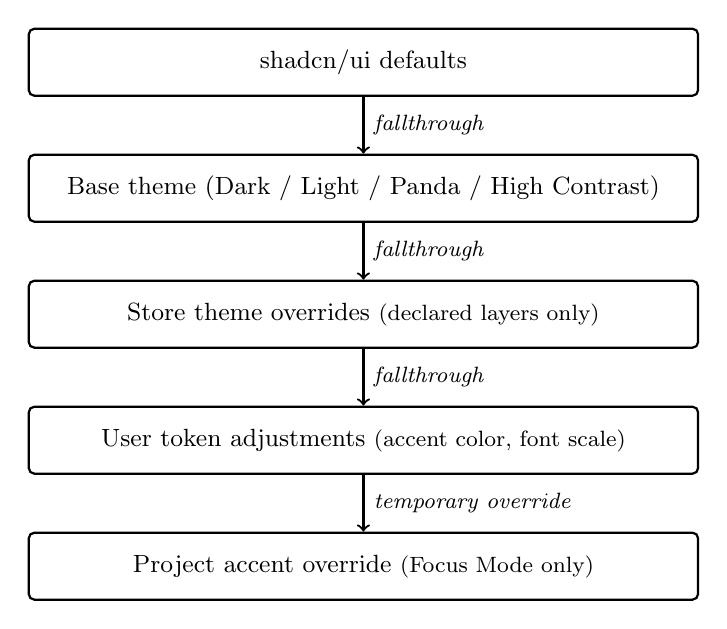
\begin{tikzpicture}[
	box/.style={
		draw, thick, rectangle, rounded corners=2pt,
		minimum width=8.5cm, minimum height=0.85cm,
		font=\small, align=center, inner sep=5pt
	},
	arr/.style={->, thick},
	lbl/.style={font=\footnotesize\itshape, anchor=west},
	]
	\def\sep{1.6}
	\node[box] (shadcn) at (0, 3*\sep)
	{shadcn/ui defaults};
	\node[box] (base)   at (0, 2*\sep)
	{Base theme (Dark / Light / Panda / High Contrast)};
	\node[box] (store)  at (0, \sep)
	{Store theme overrides \footnotesize(declared layers only)};
	\node[box] (user)   at (0, 0)
	{User token adjustments \footnotesize(accent color, font scale)};
	\node[box] (proj)   at (0, -\sep)
	{Project accent override \footnotesize(Focus Mode only)};
	\draw[arr] (shadcn) -- node[lbl, right] {fallthrough} (base);
	\draw[arr] (base)   -- node[lbl, right] {fallthrough} (store);
	\draw[arr] (store)  -- node[lbl, right] {fallthrough} (user);
	\draw[arr] (user)   -- node[lbl, right] {temporary override} (proj);
\end{tikzpicture}
\caption{Theme inheritance chain. Each layer overrides only what it declares;
everything else falls through to the layer below. The project accent override
is the outermost layer and applies only while Focus Mode is active; it is
removed when the project is deactivated, restoring the user's configured
accent. A Store theme that covers only the shell and GTK4 leaves Wine and Qt
at the base theme.}
\label{fig:theme-chain}
\end{figure}

\section{Apps, Modules, and the Store}
\label{sec:apps-modules}

\subsection{App Ecosystem}
\label{sec:app-ecosystem}

The application layer divides cleanly into two categories: first-party
applications built as part of this project, and the broader ecosystem of
third-party Linux software. Both operate under the same permission system and
benefit from the same infrastructure, but they differ in how deeply they
integrate with the platform.

\paragraph{First-party applications.}
All core system applications are built with the standard stack: Tauri, ui-kit,
and os-sdk. Each one follows the shared design language, implements an MCP
server for AI integration, emits structured events to the Event Bus, and uses
the shared TOML configuration system. Table~\ref{tab:first-party} lists the
planned core applications.

\begin{table}[htbp]
\caption{First-party system applications}
\label{tab:first-party}
\begin{tabularx}{\linewidth}{lX}
\toprule
\textbf{Application} & \textbf{Notes} \\
\midrule
File Manager    & Graph-aware features: recent files by project, related files sidebar \\
Terminal        & MCP server exposing command history and session output \\
Settings        & System-wide configuration: theming, permissions, AI level, accounts \\
Store           & App and module discovery, installation, and updates \\
Text Editor     & Basic editor primarily for configuration files \\
System Monitor  & Process list, resource usage, and Anomaly Detector alerts \\
Wine Manager    & Prefix management, Winetricks access, per-prefix version selection \\
\bottomrule
\end{tabularx}
\end{table}

\paragraph{Third-party integration layers.}
Third-party applications are not rewritten. Integration happens in four layers
of increasing depth, each building on the one below.

At the baseline, every application on the system receives passive tracking via
eBPF regardless of whether it does anything to support this platform: file
access, network connections, and process lifecycle are recorded automatically.
No changes to the application are required.

For applications that produce useful log output, a wrapper captures stdout and
stderr and passes them through asynchronous LLM extraction to produce graph
entities. These wrappers are shipped alongside packages in the package manager
where practical, and the extraction runs in the background without blocking
anything.

For popular applications, dedicated MCP server wrappers expose structured
interfaces to the AI layer. These are maintained as separate packages and
where possible contributed back to the community as independently useful tools.

Finally, applications that explicitly support the platform APIs emit structured
typed events directly to the Event Bus and implement native MCP servers. This
is the long-term goal for major open-source applications but is not a
precondition for any of the layers above it.

\paragraph{Shared standards.}
Applications that choose to integrate with the platform work with a common set
of conventions: TOML configuration files under
\texttt{\textasciitilde/.config/<app-id>/}, CSS custom properties from the
token system for applications that render via WebView, the standard
notification daemon via the Freedesktop D-Bus interface or the Event Bus for
richer notifications, and a published MCP server interface specification.

\subsection{Notification System}
\label{sec:notifications}

The Notification Daemon is the single entry point for all notifications from
all sources. Figure~\ref{fig:notifications} shows the pipeline.

\begin{figure}[htbp]
\centering
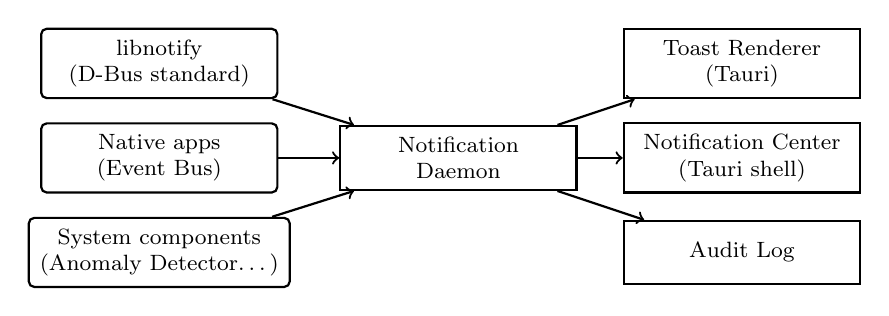
\begin{tikzpicture}[
  src/.style={
    draw, thick, rectangle, rounded corners=2pt,
    minimum width=3.0cm, minimum height=0.8cm,
    font=\footnotesize, align=center, inner sep=4pt
  },
  proc/.style={
    draw, thick, rectangle,
    minimum width=3.0cm, minimum height=0.8cm,
    font=\footnotesize, align=center, inner sep=4pt
  },
  store/.style={
    draw, thick, cylinder, shape border rotate=90,
    minimum width=1.8cm, minimum height=0.8cm,
    font=\footnotesize, align=center, inner sep=4pt
  },
  arr/.style={->, thick},
]

\node[src]  (dbus)   at (0,  2.4) {libnotify\\(D-Bus standard)};
\node[src]  (native) at (0,  1.2) {Native apps\\(Event Bus)};
\node[src]  (system) at (0,  0.0) {System components\\(Anomaly Detector\ldots)};

\node[proc] (nd)     at (3.8, 1.2) {Notification\\Daemon};

\node[proc]  (toast) at (7.4,  2.4) {Toast Renderer\\(Tauri)};
\node[proc]  (nc)    at (7.4,  1.2) {Notification Center\\(Tauri shell)};
\node[proc] (al) at (7.4, 0.0) {Audit Log};

\draw[arr] (dbus)   -- (nd);
\draw[arr] (native) -- (nd);
\draw[arr] (system) -- (nd);
\draw[arr] (nd)     -- (toast);
\draw[arr] (nd)     -- (nc);
\draw[arr] (nd)     -- (al);

\end{tikzpicture}
\caption{Notification pipeline. All sources converge on the Notification Daemon,
which normalizes, groups, and applies priority logic before forwarding to the
toast renderer and notification center. Every notification is logged in the
Audit Log by sender and timestamp, never by content.}
\label{fig:notifications}
\end{figure}

The daemon receives from two sources: the standard D-Bus interface at
\texttt{org.freedesktop.Notifications}, which means every third-party
application using \texttt{libnotify} or \texttt{notify-send} works without
changes; and the Event Bus, through which native system components send richer
notifications with priority metadata and graph context. Both are normalized to
a common internal schema before any further processing.

\begin{table}[htbp]
\caption{Notification priority levels}
\label{tab:notifications}
\begin{tabularx}{\linewidth}{lXX}
\toprule
\textbf{Level} & \textbf{Behavior} & \textbf{Do Not Disturb} \\
\midrule
Critical & Persistent toast, no auto-close &
  Always shown, never silenced \\
High     & Toast auto-closes after approximately 8 seconds &
  Delayed, not blocked \\
Normal   & Toast auto-closes after approximately 4 seconds &
  Silenced \\
Low      & No toast; goes silently to Notification Center only &
  Silenced \\
\bottomrule
\end{tabularx}
\end{table}

Critical priority is reserved for system-level alerts only: Anomaly Detector
warnings, component compatibility failures, and security events. Applications
cannot self-assign Critical. Notifications from the same application are
grouped in the Notification Center; as a toast, only the most recent
notification from an application is shown, with a counter if a previous one
from the same application is still visible. Do Not Disturb has three modes
(off, on, and scheduled by time of day) and is togglable from the taskbar quick
panel.

Focus Mode (Section~\ref{sec:focus-mode}) interacts with the notification
priority system directly. When a project declares a \texttt{[focus]} block
with \texttt{suppress\_notifications\_from}, the daemon demotes matching
application notifications to Low priority for the duration of the focused
session. This demotion is applied by the daemon at routing time, not by
modifying the application's permanent permission profile. Critical-priority
alerts from system components are exempt and always pass through regardless
of Focus Mode state.

\subsection{Permission System}
\label{sec:permissions}

Every application on the system, whether a first-party app, a Flatpak, or an
RPM package, operates within a permission profile that defines what it can
access. The system is unified: one file format, one enforcement layer, one
place for the user to review and adjust everything.

\paragraph{Permission file format.}
Each application has a TOML permission file at
\texttt{\textasciitilde/.config/permissions/<app-id>.toml} that serves as the
sole source of truth for what that application is allowed to do. The file is
human-readable and user-editable; the Settings app provides a UI for those who
prefer not to edit it directly. Permissions are enforced via Linux namespaces,
AppArmor, and seccomp, described in Section~\ref{sec:security}.

\begin{lstlisting}[language=bash, caption={Example permission file}]
# ~/.config/permissions/org.mozilla.firefox.toml

[filesystem]
allow = ["~/Downloads", "~/Documents", "~/.mozilla"]

[network]
allow = ["full"]

[devices]
allow = ["gpu"]

[graph]
# no entry = no access, never prompted
\end{lstlisting}

Graph access is never inferred or learned. An application with no
\texttt{[graph]} section has no graph access, with no exceptions and no
automatic prompting. Graph permissions must be explicitly declared.

\paragraph{Store-supplied profiles.}
The Store ships a curated permission profile alongside known applications.
Common software such as Firefox, LibreOffice, and VLC has community-maintained
profiles that are installed automatically and shown to the user at install time
for review. Community members can submit profiles for applications not yet
covered; submitted profiles go through Store review before publication, since
an overly permissive profile is a meaningful risk. Permission profiles are one
component of the broader Integration Package system described in
Section~\ref{sec:integration-packages}.

\paragraph{Flatpak adapter.}
Flatpak applications carry their own permission declarations. When a Flatpak is
installed, the system automatically generates a native permission file by
mapping Flatpak permissions to the native format: \texttt{filesystem=home}
becomes \texttt{filesystem.allow = ["\textasciitilde/"]}, and so on. The
generated file is shown to the user at install time and can be tightened before
confirming. The Flatpak manifest is the floor; the system never grants more
than what the Flatpak declared.

\paragraph{First-run learning mode.}
If no Store profile exists and the application is not a Flatpak, the first
launch runs in learning mode: all accesses are permitted and logged, nothing is
blocked. The learning window closes automatically ten minutes after first
launch, or when the session ends, whichever comes first. The user then receives
a summary of what the application accessed, with options to review and confirm,
edit first, or start with all permissions blocked. From the second launch
onward, the confirmed profile is enforced. Learning mode applies to filesystem,
network, and device access only; graph access is always denied until explicitly
granted and cannot be learned. During the learning window, at most five new
permission grants are recorded per minute; exceeding this rate suspends
learning immediately and generates an anomaly alert. This limits the damage
from a compromised application that attempts to accumulate permissions in bulk
during its first session.

\paragraph{Runtime behavior.}
When an application attempts an access outside its profile, the access is
denied and the user receives a notification offering to extend the profile.
If the user allows, the profile is updated and the application retries the
action; if the user denies, the block stands. Repeated denials for the same
path are collapsed: after three denials for the same access, the system asks
once whether to always block it rather than continuing to prompt.

\paragraph{Ephemeral app mode.}
Any application can be launched in ephemeral mode, either from the right-click
context menu in the launcher or via a command-line flag. Ephemeral mode
combines several existing sandbox mechanisms into a single preset with no
configuration required.

In ephemeral mode, a private Mount Namespace is created with no write access
to the home directory; the application sees a temporary overlay that is
discarded on exit. Graph access is entirely disabled regardless of the
application's normal permission profile. Network activity is permitted if
declared in the application manifest, but is not logged to the Audit Log.
On exit, the temporary overlay is deleted, no entries are written to the
Knowledge Graph, and no permission changes persist.

The intended use case is opening untrusted or one-off content: a PDF from an
unknown sender, a binary downloaded for a single use, or any application the
user wants to run without leaving a trace. Ephemeral mode is not a replacement
for the full profile isolation that separate Linux users provide; it does not
protect against a compromised application exploiting a kernel vulnerability.
What it provides is a low-friction way to reduce the footprint of routine
untrusted content without requiring a separate session or a virtual machine.

\subsection{Integration Packages}
\label{sec:integration-packages}

An Integration Package is a Store package that describes how the system
integrates with a specific third-party application. It is not a bundle: it
contains no application binaries. It is a declaration that references an
existing application and provides three optional components alongside it:
a permission profile, a Settings adapter, and native Settings registrations
for os-sdk applications.

The application itself and its Integration Package are two independent Store
entries with separate versions, separate maintainers, and separate update
cycles. A package published by Mozilla ships Firefox; an Integration Package
published by the community ships the permission profile and Settings adapter
for Firefox.

\paragraph{Package format.}
An Integration Package declares which application it targets and what it
provides:

\begin{lstlisting}[language=bash, caption={Integration Package manifest}]
[package]
id      = "community.firefox.integration"
name    = "Firefox Integration"
version = "2.1.0"
conflicts = ["community.firefox.privacy"]

[app]
# At least one identifier required; all three are optional
store_id     = "org.mozilla.firefox"
flatpak_id   = "org.mozilla.Firefox"
package_name = "firefox"

# Compatible with which app versions
compatible_with = ">=120.0, <130.0"

[includes]
permissions = "permissions.toml"   # optional
adapter     = "firefox-adapter.toml"  # optional
\end{lstlisting}

The \texttt{conflicts} field lists Integration Packages that are incompatible
with this one. When the Store detects a conflict at install time, it presents
the user with a choice rather than silently merging or overriding. If both
packages are installed simultaneously (for example via a package manager), the
Settings page for the affected application shows a conflict warning and the
permissions of the first-installed package remain active until the user
resolves the conflict.

\paragraph{Settings Adapter.}
The Settings Adapter is a declarative TOML document that describes how a
third-party application's native configuration file maps to Settings UI
elements. It contains no executable code; Settings interprets the declaration
and performs all reads and writes itself.

\begin{lstlisting}[language=bash, caption={Settings Adapter declaration}]
[adapter]
schema_version = "1.0"
write_strategy = "requires_app_closed"  # or "anytime"

[sources]
prefs = {
    path              = "~/.mozilla/firefox/*/prefs.js",
    format            = "firefox-prefs",
    instance_strategy = "last_used"  # or "all", "ask"
}

[[settings]]
key      = "browser.startup.homepage"
source   = "prefs"
label    = "Homepage"
type     = "string"
default  = "about:home"
section  = "General"
verify   = true

[[settings]]
key      = "browser.tabs.tabMinWidth"
source   = "prefs"
label    = "Minimum tab width"
type     = "integer"
min      = 50
max      = 250
default  = 76
section  = "Tabs"
readonly = false

[[settings]]
key      = "browser.cache.disk.capacity"
source   = "prefs"
label    = "Disk cache size (internal)"
type     = "integer"
section  = "Advanced"
readonly = true
\end{lstlisting}

\emph{write\_strategy} controls when Settings may write to the configuration
file. \texttt{anytime} writes immediately; \texttt{requires\_app\_closed}
disables all edit controls while the application is running and writes only
when it is not, because some applications overwrite their configuration on
exit and would discard changes made while running.

\emph{instance\_strategy} applies when the source path glob matches multiple
files. \texttt{last\_used} selects the file with the most recent modification
timestamp, appropriate for applications that maintain separate profiles.
\texttt{all} writes to every matched file simultaneously. \texttt{ask}
prompts the user once on the first opening of the Settings page and remembers
the selection.

\emph{verify} causes Settings to read the field back after writing and compare
it to the value it attempted to write. If the values do not match, Settings
displays an error rather than silently succeeding. This catches cases where an
application has renamed or removed a configuration key in a newer version.

\emph{readonly} fields are displayed but not editable. They carry a lock
indicator in the Settings UI.

The adapter supports the following configuration formats via built-in format
handlers: TOML, JSON, INI and \texttt{.conf} files, Firefox \texttt{prefs.js},
\texttt{.env} key-value files, and flat \texttt{key=value} files. Binary and
proprietary formats are not supported; the application page in Settings shows
only the Permissions section when no compatible adapter is available.

Adapter source files are restricted to paths within known user configuration
directories. An adapter cannot declare a source outside \texttt{\textasciitilde/.config/},
\texttt{\textasciitilde/.mozilla/}, \texttt{\textasciitilde/.local/}, and
similar user-owned paths. System paths are never writable through an adapter.

\paragraph{Compatibility and updates.}
The \texttt{compatible\_with} field declares which application versions the
Integration Package supports. When the application updates beyond the declared
range, Settings displays a compatibility warning on the application page with
a direct link to the Store listing of the Integration Package. The adapter
remains active -- most configuration keys do not change between application
versions -- but the warning signals that the package maintainer should review
and update the package.

Integration Package updates are independent of application updates. The Install
Daemon (Section~\ref{sec:install-daemon}) monitors both streams and keeps
them consistent.

\paragraph{Native app Settings registration.}
First-party applications built with os-sdk do not use the adapter mechanism.
They register their Settings interface directly at startup via os-sdk, using
the same TOML configuration system the application already uses internally.
There is no configuration file bridge and no format handler involved:

\begin{lstlisting}[language=bash, caption={Native Settings registration via os-sdk (TypeScript)}]
shell.settings.register({
  sections: [
    {
      label: "General",
      items: [
        {
          key:     "startup.restore_session",
          label:   "Restore last session on startup",
          type:    "boolean",
          default: true,
        },
        {
          key:     "editor.font_size",
          label:   "Font size",
          type:    "integer",
          min:     8,
          max:     32,
          default: 14,
        },
        {
          key:     "editor.theme",
          label:   "Editor color scheme",
          type:    "enum",
          options: ["system", "dark", "light"],
          default: "system",
        },
      ]
    }
  ]
})
\end{lstlisting}

Settings reads this registration and renders the application's configuration
section automatically. Values are read from and written to the application's
own \texttt{\textasciitilde/.config/<app-id>/config.toml} via the os-sdk
configuration system. The application observes changes via the same inotify
mechanism all other components use. No adapter, no format handler, no
intermediate layer.

The distinction between the two paths is clean: the adapter is for existing
third-party applications that the system does not control; native registration
is for applications built for this platform that already use os-sdk.

\subsection{Install Daemon}
\label{sec:install-daemon}

The Install Daemon is a background service that sits as an abstraction layer
over all package managers active on the system. Its role is to ensure that
every application installation, regardless of how it was performed, results in
a consistent system state: permissions enforced, Integration Package loaded
if available, Settings page populated.

A user who types \texttt{dnf install firefox} in a terminal has the same
expectation as a user who finds Firefox in the Store: the application works,
its permissions are set to sensible defaults, and its Settings page is ready.
The Install Daemon makes that expectation true regardless of installation path.

\paragraph{Package manager coverage.}
The daemon registers hooks with all package managers it finds on the system.
For systemd-integrated package managers (dnf, Flatpak), it uses systemd unit
hooks that emit an Event Bus message after every install, update, or removal.
For non-systemd package managers (Homebrew, Nix, Cargo, pip with
\texttt{-{}-user}), it monitors known installation paths via
\texttt{inotify}:

\begin{lstlisting}[language=bash, caption={Monitored installation paths}]
~/.homebrew/        ~/.nix-profile/
~/.cargo/bin/       ~/.local/bin/
/opt/homebrew/
\end{lstlisting}

New package managers installed after first login are detected when their binary
appears in a known package manager location. From that point the daemon begins
monitoring their output paths as well.

When the daemon detects a new application it cannot associate with a known
app-ID, it takes no action. Only positively identified applications trigger
Integration Package lookup.

\paragraph{Integration Package matching.}
After detecting a new application installation, the daemon queries the Store
catalogue for Integration Packages that reference the installed app-ID via
any of the three reference fields (\texttt{store\_id}, \texttt{flatpak\_id},
\texttt{package\_name}). Matching packages are evaluated against a three-tier
rating policy:

\begin{table}[htbp]
\caption{Install Daemon Integration Package rating policy}
\label{tab:install-rating}
\begin{tabularx}{\linewidth}{lX}
\toprule
\textbf{Condition} & \textbf{Behavior} \\
\midrule
Rating $\geq$ 4.0 and installs $\geq$ 1{,}000 &
  Installed automatically. Brief notification after completion. \\
Rating 3.0--3.9 or installs $<$ 1{,}000 &
  Notification with Install button. Not automatic. \\
Rating $<$ 3.0 or installs $<$ 100 &
  Not surfaced. Available in the Store via manual search. \\
\bottomrule
\end{tabularx}
\end{table}

If only one Integration Package exists for an application and it does not
meet the automatic threshold, the minimum rating for automatic installation
is lowered to 3.5. No Integration Package is worse than a completely absent
one from a user experience perspective.

\paragraph{Dual installation handling.}
When the same application exists as both an RPM and a Flatpak, the daemon
treats them as two separate entries. Settings shows both with distinct labels
(for example ``Firefox (System)'' and ``Firefox (Flatpak)'') and separate
application pages. The user designates one as primary in Settings; the primary
installation is used for default application associations and Waypointer
suggestions.

\paragraph{Offline queue.}
When an application is installed without network access, the daemon stores a
pending lookup entry locally. The next time the network becomes available --
detected via a NetworkManager event on the Event Bus -- the daemon processes
queued entries and applies the normal matching policy. Queue entries expire
after 30 days without resolution.

\paragraph{Update compatibility.}
Application updates are never blocked by Integration Package compatibility
status. When an application updates beyond an Integration Package's declared
\texttt{compatible\_with} range, the daemon checks the Store for a newer
version of the Integration Package. If one exists it is installed
automatically. If none exists, Settings displays a compatibility warning. The
application update proceeds regardless.

\paragraph{Deinstallation.}
When an application is removed, its Integration Package is set to inactive
rather than uninstalled. It remains visible in a dedicated ``Inactive
Integrations'' section of Settings. If the application is reinstalled, the
Integration Package reactivates automatically without prompting. Explicit
removal of the Integration Package is a separate user action available from
the inactive list or the Store.

\paragraph{Audit log.}
Every Install Daemon action is recorded in the Audit Log via the Audit Daemon:
automatic Integration Package installations, manual installations triggered by
notification, deactivations, reactivations, and failed queue resolutions. Each
entry carries the app-ID, Integration Package ID and version, trigger source,
rating and install count at decision time, and whether the action was automatic
or user-initiated.

The system is extensible at multiple layers through a unified module mechanism.
All module types use the same installation channel (the Store) and the same
manifest format, but they operate as independent subsystems with separate APIs.
A single Store package can bundle multiple module types together.

\paragraph{Module categories.}
Table~\ref{tab:modules} lists the available extension points. Theme modules
are a special case: they consist of CSS and token overrides only, contain no
executable code, and require no sandbox. All other categories run sandboxed
with declared permissions.

\begin{table}[htbp]
\caption{Module categories and extension points}
\label{tab:modules}
\begin{tabularx}{\linewidth}{llX}
\toprule
\textbf{Category} & \textbf{Extension point} & \textbf{Example} \\
\midrule
\texttt{theme}               & Design language layer     & Community color schemes \\
\texttt{waypointer.provider} & Waypointer search results & Web search, stock prices \\
\texttt{waypointer.action}   & Waypointer command actions & Create task, send message \\
\texttt{shell.topbar}        & Topbar element slot       & Custom status widget \\
\texttt{shell.widget}        & Desktop widget area       & Clock, weather, system stats \\
\texttt{mcp.server}          & AI MCP integration        & External service connector \\
\texttt{keybinding.profile}  & Global input manager      & Alternative layout profiles \\
\bottomrule
\end{tabularx}
\end{table}

\paragraph{Manifest format.}
Every module package has a single manifest that declares what it provides,
its dependencies, conflicts, and permissions. The \texttt{[permissions]} block
uses the same schema as application permission files; at install time the
Module Runtime generates the permission file from the manifest and the user can
inspect and adjust it in Settings like any other application.

\begin{lstlisting}[language=bash, caption={Example module manifest}]
[package]
id      = "com.example.ai-waypointer"
name    = "AI Waypointer Provider"
version = "1.0.0"

[provides]
waypointer.provider = true

[activation]
# Optional: only run this module when a focused project carries these tags.
# The Module Runtime starts and stops the module as Focus Mode changes.
# Omit this block for modules that run unconditionally.
active_when_focused = { require_tags = ["rust"] }

[dependencies]
shell   = ">=1.2"
modules = ["com.example.ai-core"]

[permissions]
network.allow = ["api.openai.com"]
graph.allow   = ["read"]
\end{lstlisting}

The \texttt{[activation]} block is optional. When present, the Module Runtime
evaluates it against the active \texttt{Project} node each time Focus Mode
changes. A module with \texttt{require\_tags = ["rust"]} is started when the
focused project carries the \texttt{rust} tag and stopped when Focus Mode
deactivates or switches to a project that does not. The module's declared
permissions apply for the duration it is running; they are not expanded or
restricted by the activation condition. A module started via project activation
follows the same crash recovery policy as any other module.

Modules cannot declare permissions beyond what the manifest specifies, and
manifests are reviewed during Store submission. Unlike applications, modules
cannot expand their permissions at runtime through a learning mode; their
profile is set at install time and any undeclared access returns
\texttt{EACCES}.

\paragraph{Module Runtime.}
A dedicated Module Runtime daemon manages lifecycle, sandboxing, and crash
recovery for all active modules. Each module runs in its own isolated WebView
context, separate from the shell's WebView. A module crash does not affect the
shell or other modules.

The runtime uses exponential backoff per module instance for crash recovery,
shown in Table~\ref{tab:crash-recovery}. The 60-second window resets on a
clean run, so a module that runs for several minutes and then crashes once
gets an immediate restart.

\begin{table}[htbp]
\caption{Module crash recovery policy}
\label{tab:crash-recovery}
\begin{tabularx}{\linewidth}{lX}
\toprule
\textbf{Crash count (within 60 s)} & \textbf{Behavior} \\
\midrule
1st & Immediate restart \\
2nd & Restart after 5 seconds \\
3rd & Restart after 30 seconds \\
4th or more & Marked as failed; no further automatic retries \\
\bottomrule
\end{tabularx}
\end{table}

When a module is marked failed, Settings shows a subtle error indicator with
the last crash log. The user can trigger a manual retry at any time. There is
no notification spam.

Module updates are downloaded in the background and applied at different points
depending on category: theme updates apply immediately as a token and CSS swap;
Waypointer modules update on the next Waypointer open; shell widgets and topbar
modules update on the next session start by default, with a manual
``Restart now'' option available in Settings; MCP server modules update on the
next session start to avoid interrupting active AI interactions.

\paragraph{Shell API.}
Modules interact with the system through a restricted TypeScript SDK. No direct
access to the compositor or Graph Daemon is available; what is not in
the SDK is not accessible.

\begin{lstlisting}[language=bash, caption={Module SDK surface (TypeScript)}]
import { shell } from "@os/module-sdk"

// Window management
const windows = await shell.getWindows()
const active  = await shell.getActiveWindow()

// Graph (requires graph = "read" in manifest)
const recent = await shell.graph.query(
  "MATCH (f:File) RETURN f LIMIT 5"
)

// Waypointer provider registration
shell.waypointer.register({
  id:          "com.example.ai-waypointer",
  placeholder: "Ask AI...",
  onQuery:     async (q) => [ /* result objects */ ]
})

// Focus Mode: react to project context changes
shell.focus.onActivate((project) => {
  // project.name, project.tags, project.rootPath available
})
shell.focus.onDeactivate(() => { /* cleanup */ })
\end{lstlisting}

The \texttt{shell.focus} API allows modules to react to Focus Mode transitions
without polling. A Waypointer provider that wants to narrow its result set to
the active project subscribes to \texttt{onActivate} and adjusts its query
scope accordingly; \texttt{onDeactivate} signals that the module should return
to its default behavior. These callbacks fire after all system-level Focus Mode
changes have been applied, so the project context is already consistent when
the module receives the event.

\paragraph{Global Input Manager.}
Keybindings and gestures are configured in a single place in Settings, not per
application or per module. Modules register named actions with default
bindings; the user overrides them centrally. The module never receives the
binding string directly; the Input Manager calls the registered action handler
when the binding fires. This means a user can rebind everything from one place
and no module can silently capture input outside its declared actions.

\paragraph{Developer experience.}
A CLI scaffolds a complete module project with one command:
\texttt{npx create-os-module <n>}, producing a Vite, TypeScript, Tailwind,
and module-sdk setup with a manifest template. In dev mode, the module runs
unsigned in a dedicated dev sandbox, all declared permissions are granted
without Store review, WebView DevTools are accessible, and hot-reload via Vite
is active. Dev mode is only available on developer builds; production builds
reject unsigned modules.

For distributing a finished module outside the Store, a developer generates a
self-signed key pair with the CLI, signs the module, and distributes it as an
\texttt{.osmod} file. Installation uses TOFU: the first install prompts the
user to trust the key fingerprint; subsequent updates from the same key are
silent. Sideloaded modules receive no expanded permissions and are marked
``Not from Store'' in Settings.

\subsection{Store}
\label{sec:store}

The Store is the primary distribution channel for applications, themes,
modules, and profile packages. It is designed to be financially sustainable for
the project without becoming a gatekeeper for the ecosystem.

\paragraph{Publishing.}
Publishing an application to the Store is free and remains free indefinitely.
There is no annual developer fee. Every upload runs automated technical checks:
valid permission declarations, correct package signing, sandbox policy
compatibility, and resolvable declared dependencies. These checks are
automated; no manual review is required for packages that pass them. A failed
check returns a specific error. A manual Security Review is available
optionally and is the basis for the Security Audit Badge described below.

\paragraph{Revenue model.}
Supported pricing models include free, one-time purchase, subscription,
in-app purchases, pay-what-you-want, and freemium. Developers can also direct
users to external payment links; the Store payment infrastructure is a
convenience, not a monopoly.

Commission is calculated on total annual revenue across all applications in a
developer account, using the tiered structure in Table~\ref{tab:commission}.
When a threshold is crossed mid-year, the new rate applies to all subsequent
transactions in that year, not retroactively.

\begin{table}[htbp]
\caption{Store commission tiers}
\label{tab:commission}
\begin{tabularx}{\linewidth}{XX}
\toprule
\textbf{Annual revenue (account total)} & \textbf{Commission} \\
\midrule
Up to \EUR{10,000}                        & 0\% \\
\EUR{10,000} to \EUR{50,000}              & 5\% \\
\EUR{50,000} to \EUR{500,000}             & 15\% \\
\EUR{500,000} to \EUR{5,000,000}          & 20\% \\
Over \EUR{5,000,000}                      & 25\% \\
\bottomrule
\end{tabularx}
\end{table}

\paragraph{User-facing features.}
Purchases are tied to the user account, not the device. Trials are declared in
the app manifest and enforced by the Store; no credit card is required to start
a trial, and when it ends the user receives a single notification with a
purchase option and no automatic charges. Family Sharing is opt-in per
application: developers can allow up to six to eight family members to use an
application under one purchase. Every application's Store page shows a full
price history including every price change with its date; this is automatic and
cannot be disabled by the developer. All active subscriptions across all
applications are visible and cancellable in one place in Settings.

\paragraph{Developer dashboard.}
Developers see install counts, active user numbers, revenue and payout history,
ratings and written reviews, crash reports from users who opted into crash
reporting at the system level, and version adoption numbers. All data is
aggregated and anonymized; the developer sees counts, never identities. No
third-party analytics are required or supported.

\paragraph{Security Audit Badge.}
Applications can display a Security Audit badge on their Store page by
uploading an independent security audit report. The Store verifies that the
report originates from the stated auditing organization and links it from the
application page. Users can read the full report and judge the auditing
organization's credibility themselves. The badge means an audit exists and is
accessible, not that the Store has endorsed the application's security.

\paragraph{Long-term support.}
Developers can declare a Long Term Support commitment in the application
manifest by setting a support end date. The Store displays this date publicly
on the application page. It is a voluntary public commitment with no automated
enforcement, but the public visibility creates accountability. LTS applications
are filterable in Store search for users who prioritize stability.

\paragraph{Profile package distribution.}
Signed environment profile packages (\texttt{.lenv} files, described in
Section~\ref{sec:platform}) are distributed through the Store using the same
infrastructure as applications. Profile packages are free to publish and carry
no commission.

\paragraph{Integration Package distribution.}
Integration Packages (described in Section~\ref{sec:integration-packages}) are
distributed through the Store as a distinct package type. They are free to
publish and carry no commission. Publishing runs the same automated technical
checks as applications: valid signing, resolvable app references, and schema
validation of any included adapter declaration. A manual Security Review is
available and recommended for packages that include permission profiles, since
an overly permissive profile represents a meaningful risk.

Store listings for Integration Packages display the target application, the
package components included (permissions, adapter, or both), the
\texttt{compatible\_with} version range, and the standard rating and install
count. The Install Daemon uses rating and install count to determine automatic
installation eligibility as described in Section~\ref{sec:install-daemon}.

Deep links between Integration Package Store listings and the corresponding
application page in Settings use the \texttt{store://} and \texttt{settings://}
URL schemas described in Section~\ref{sec:settings-deeplinks}.

\section{Platform, Profiles, and Security}
\label{sec:platform}

\subsection{Account System}
\label{sec:accounts}

The Account System is the single place where the user manages all online
accounts and external service connections. Set up once, available everywhere,
with full visibility into which application accesses what. The design principle
is straightforward: no application ever directly handles OAuth flows, stores
tokens, or manages credentials. All credential logic lives in a dedicated
\emph{Account Daemon}.

The daemon serves two related but distinct purposes. First, it manages
user-facing online accounts such as Google, Microsoft, and Nextcloud, including
OAuth flows, token refresh, and the GNOME Online Accounts bridge. Second, it
manages the credentials for external service Connections configured in Settings
(Section~\ref{sec:connections}): GitHub, GitLab, n8n, OpenClaw, and any other
Connection the user creates. Both credential types live in the Linux Kernel
Keyring and are accessed exclusively through the daemon. No other component
reads credentials from the Keyring directly.

\emph{OAuth~2.0}~\cite{rfc6749} is the standard authorization framework used
by cloud services to grant third-party applications access to user data without
sharing the user's password. The flow works by redirecting the user to the
service's login page, where they authenticate and approve a specific set of
\emph{scopes} (declared permissions such as ``read email'' or ``write
calendar''), after which the service issues a short-lived \emph{access token}
and a long-lived \emph{refresh token}. The access token is sent with each API
request; the refresh token is used to obtain new access tokens when the current
one expires. An application that holds both tokens has persistent access to the
user's account; protecting them is therefore critical.

\paragraph{Architecture.}
Applications declare what they need; the daemon handles the rest. When an
application needs access to a service, it sends a request to the Account
Daemon, which checks the application's permission profile, retrieves or
derives the appropriate token, logs the access in the Audit Log, and returns
what the application needs. The application then communicates with the
provider's API directly using that token. The daemon is the sole keeper of
all credentials; tokens never live in application memory longer than
necessary.

\paragraph{Service-level permissions.}
Applications request access at the service level, not the OAuth scope level.
The user sees human-readable service names and never raw OAuth scope strings.
When an application requests account access for the first time, the user sees
exactly which service is being requested, grants or denies it, and the
decision is stored in the application's unified permission profile as described
in Section~\ref{sec:permissions}. Account permissions are part of the same
system as filesystem, network, and graph permissions.

\begin{lstlisting}[language=bash, caption={Service-level permission view (Settings)}]
Google Account (personal@example.com)
  Mail      -> allowed for: Thunderbird
  Calendar  -> allowed for: Calendar App, AI daemon (read-only)
  Drive     -> allowed for: File Manager
  Contacts  -> not granted to anyone
\end{lstlisting}

\paragraph{Multiple accounts and resolution order.}
When multiple accounts of the same type exist, the system resolves which to
use via a three-tier model. The system default applies globally; an Isolated
Desktop context can declare its own defaults, so that switching to the Work
desktop automatically switches the active account context; and individual
applications can be manually pointed at a specific account regardless of the
desktop context. Resolution proceeds from most specific to least specific:
per-app override, then desktop default, then system default.

\begin{lstlisting}[language=bash, caption={Account resolution configuration}]
# resolved in order: per-app override -> desktop default -> system default
[defaults]
google = "personal@example.com"

[desktop.work.defaults]
google = "work@example.com"

[app."org.mozilla.thunderbird"]
# always uses personal account regardless of active desktop
google = "personal@example.com"
\end{lstlisting}

\paragraph{Token security.}
Credentials never leave the Account Daemon as-is. Two paths are used
depending on provider support. For providers that support OAuth scope
restriction, the daemon issues a short-lived derived token scoped only to
what the application declared, with a default lifetime of five minutes. The
full OAuth token and refresh token never leave the daemon at all. For
providers that do not support downscoping, the full token is handed to the
application but with two compensating controls: every token handoff is logged
in the Audit Log, and tokens are actively revoked when the application process
exits. All credentials at rest are stored in the Linux Kernel Keyring~\cite{archwiki:keyring}: a kernel-managed storage
area for cryptographic keys, tokens, and passwords that lives in kernel memory
rather than userspace files, making it inaccessible to other processes and not
visible in \texttt{/proc} or on disk. The daemon
loads them into memory only when actively needed and discards them immediately
after.

\paragraph{Offline behavior.}
Two failure modes are handled distinctly. When the provider rejects the token
because the user revoked access or the account password changed, the daemon
emits a single system notification directing the user to Settings and does not
repeat it; applications receive a clear \texttt{AccountAuthRequired} error
code and surface a gentle in-app hint. When the network itself is unavailable,
the daemon serves cached data from the last successful sync, clearly marked
with the timestamp of the last update. A calendar application shows last-known
events labeled with their age rather than an empty state. When connectivity
is restored, the daemon refreshes silently in the background and notifies
applications of updated data via the Event Bus.

\paragraph{Connection credential management.}
External service Connections configured in Settings are stored as named
entries in the Linux Kernel Keyring under the \texttt{lunaris/connections/}
namespace. The Account Daemon is the sole process that reads and writes these
entries. When a component requests the credential for a Connection it provides
the Connection identifier and its own component identity; the daemon checks
whether the requesting component is listed in the Connection's \texttt{allowed}
field before returning anything. Unauthorized requests receive
\texttt{EACCES} with no credential data.

Token refresh for Connections follows a two-path model. For providers that
issue refresh tokens alongside access tokens, the daemon attempts a silent
refresh in the background when the access token approaches expiry. If the
refresh succeeds the new token is stored in the Keyring and the Connection
continues working without interruption. If the refresh fails, or if the
provider does not issue refresh tokens at all, the daemon marks the Connection
as \texttt{expired}, returns \texttt{token\_expired} to requesting components
rather than a stale or invalid token, and sends a single High-priority
notification to the user with a deep link to
\texttt{settings://connections/<id>}. The notification is sent once and not
repeated until the user interacts with it or the Connection is renewed.

The daemon also maintains the outbound webhook endpoint whitelist for the
Event Bus. Whenever a Connection with outbound events is created, modified,
or deleted, the daemon pushes the updated whitelist to the Event Bus over a
dedicated internal channel. The Event Bus never queries the daemon at send
time; it uses the cached whitelist to avoid any latency in the hot event path.

\paragraph{GNOME Online Accounts bridge.}
\emph{GNOME Online Accounts}~\cite{gnome:goa} (GOA) is a GNOME framework
that centralizes cloud service credentials (Google, Microsoft, Nextcloud, and
others) and exposes them to applications via a D-Bus interface.
Applications built for GNOME that use GOA expect a D-Bus
interface at \texttt{org.gnome.OnlineAccounts}. The system provides a
GOA-compatible bridge that implements this interface exactly but sources all
data from the Account Daemon internally. Evolution, GNOME Calendar, and other
GOA-dependent applications work without modification. Internally every request
goes through the Account Daemon, through the permission system, and through
the Audit Log. The bridge translates; it does not add logic.

\subsection{Profile System}
\label{sec:profiles}

A profile is a complete, isolated user environment backed by a separate Linux
system user. Each profile has its own home directory, its own Knowledge Graph,
its own account configuration, and its own set of running system daemons.
Isolation is enforced at the kernel level, not by convention.

The profile system replaces the concept of isolated desktops within a session.
Rather than trying to isolate individual desktops within a single session, the
entire session is the isolation boundary. Switching profiles is a session
switch, not a window toggle.

\paragraph{Personal profiles.}
The primary profile, created at system setup, cannot be deleted. It has no
restrictions: full access to all installed applications, all accounts, and all
system features. This is the default context the user logs into.

\paragraph{Work and custom profiles.}
A user-created or organization-deployed profile for a specific context such as
work, a project, or a secondary identity. Backed by a separate Linux user with
its own encrypted home image via \texttt{systemd-homed}. Virtual desktops,
accounts, Knowledge Graph, and application configurations are all independent
from the Personal profile. Multiple custom profiles can coexist. Each is a
full Linux user; switching to one is a standard session switch with saved and
restored window state.

\paragraph{Locked profiles.}
A profile deployed by an institution for controlled sessions: exams, regulated
work environments. Backed by a temporary Linux user created at session start
and deleted when the session ends. The user cannot switch to another profile
while a Locked session is active; this is enforced at the compositor level, not
by UI alone. After the session ends, the Linux user and all associated data are
removed. No data from the Locked session survives into the Personal profile.

\paragraph{Guest mode.}
A lightweight temporary context for short-term use by another person. Unlike
other profile types, Guest does not create a second Linux user or a second
compositor session. It runs as a sandboxed environment on top of the current
session: a separate namespace, an empty home directory, no access to the host
user's data. The host session is suspended in the background and resumed
instantly when Guest ends. All Guest data is discarded on exit.

\paragraph{Technical foundation.}
Each non-Guest profile is a Linux system user. Profile creation is
\texttt{useradd} plus \texttt{systemd-homed} home image setup; profile
switching is a standard Linux user session switch; profile deletion is
\texttt{userdel} plus home image removal. Isolation is kernel-enforced.
\texttt{systemd-homed} provides per-profile LUKS-encrypted home images. When
a profile is not active, its home image is unmounted and its encryption key
is discarded from memory. Each profile runs its own instance of all system
daemons: Graph Daemon, Account Daemon, Event Bus. There is no shared daemon
state between profiles.

\paragraph{Data transfer between profiles.}
By default profiles are fully sealed from each other. Controlled data transfer
is configured per profile pair in Settings, with independent directional
control over clipboard, drag-and-drop, and a shared folder:

\begin{lstlisting}[language=bash, caption={Cross-profile transfer configuration}]
[profile.work.transfer]
clipboard              = "in-only"    # "off" | "in-only" | "out-only" | "both"
drag_drop              = "in-only"
shared_folder          = "~/Transfer/Work"
shared_folder_permission = "read-write"  # or "read-only" | "off"
\end{lstlisting}

A dedicated \emph{Transfer Daemon} is the only process with simultaneous
access to both profile namespaces. All cross-profile data flow goes through
it; nothing bypasses it. Whenever data flows out of a profile, a
non-dismissable toast appears for three seconds identifying the source profile,
destination, and file name, with an Undo option. The transfer proceeds but can
be cancelled within the window. All transfers are recorded in the Audit Log
with source, destination, transfer type, and data description.

Locked profiles have transfer hardcoded to off in all directions. This cannot
be overridden by the user or by an organization's configuration package; it is
a system-level invariant with no configuration surface.

\paragraph{Signed profile packages.}
Profiles can be deployed via a \emph{Signed Profile Package}, a
\texttt{.lenv} file created and signed by an organization. The user installs
it themselves and retains full control over their device. The organization
gets a tamper-evident, versioned configuration. This is the BYOD model: the
organization controls their context, the user controls their device.

\begin{lstlisting}[language=bash, caption={Signed profile package format}]
[environment]
id        = "com.acme.work-profile"
name      = "Acme Work"
version   = "2.1.0"
publisher = "Acme GmbH"
type      = "persistent"    # or "locked" for exam/controlled sessions

[transfer]
clipboard     = "in-only"
drag_drop     = "in-only"
shared_folder = "off"

[network]
require_vpn    = "acme-vpn"
allow_outbound = ["*.acme.com", "*.office365.com"]
block_outbound = ["*"]

[apps]
required = ["com.acme.timetracker", "org.mozilla.firefox"]
blocked  = ["com.valve.steam"]

[graph]
ai_access = "off"
export    = "off"

# Project templates bundled with this profile.
# Each entry is a path to a .project file relative to the package root.
# These are written to the profile's home directory on install and
# registered as active projects in the Knowledge Graph.
[projects]
templates = [
    "projects/acme-onboarding.project",
    "projects/acme-infrastructure.project",
]
\end{lstlisting}

Project templates bundled in the \texttt{[projects]} block are installed into
the profile's home directory at \texttt{\textasciitilde/.projects/<template-name>/}
on first login and registered as active \texttt{Project} nodes in the profile's
Knowledge Graph. Each template is a standard \texttt{.project} TOML file
(Section~\ref{sec:projects}) and follows the same format; the organization
can pre-configure name, description, tags, linked accounts, AI scope, and
Focus Mode rules. Project templates do not contain user data and are not
synchronized back to the organization; they are a starting configuration
only. The user can modify or delete them after installation without affecting
the profile package itself.

The package is signed by the organization's private key. Key distribution uses
TOFU by default: on first install the user sees the publisher name and key
fingerprint and confirms trust. For managed onboarding, IT can send an
enrollment link so that the organization's key is imported before any package
arrives, eliminating the TOFU prompt entirely.

Before installation, a full summary of every policy and restriction is shown.
Nothing is hidden. There are certain things an organization cannot do through
a signed package, enforced technically rather than by policy: the organization
cannot read the user's Personal profile or its Knowledge Graph, cannot access
any data outside the profile's Linux user boundary, cannot monitor activity
in other profiles, cannot remotely wipe or modify the device, and cannot
prevent the user from uninstalling the package. If \texttt{notify\_on\_uninstall}
was declared and accepted at install time, the organization receives a
notification when the package is removed, but the removal proceeds regardless.

\subsection{Gaming and Windows Compatibility}
\label{sec:gaming}

Gaming and Windows application compatibility are first-class features, not
afterthoughts. The required components are pre-installed and pre-configured;
no manual setup is required.

\paragraph{Wine and Proton.}
\emph{Wine} provides compatibility for Windows applications on Linux.
\emph{Proton}~\cite{proton} is Valve's fork of Wine, optimized for gaming
and maintained with extensive patches from Valve's Linux gaming team; for gaming specifically
it is substantially better than vanilla Wine. Both are pre-installed alongside
\emph{DXVK}~\cite{dxvk}, which translates Direct3D 9, 10, and 11 API
calls to Vulkan. Direct3D is the Windows graphics API; most games targeting
Windows use it rather than Vulkan directly. By translating at the API boundary,
DXVK allows these games to run on Linux via the Vulkan driver.
\emph{vkd3d-proton}~\cite{vkd3d:proton} is Valve's fork of the Wine project's
vkd3d library; it translates Direct3D 12 (the modern Windows GPU API) to
Vulkan, with extensive optimizations for gaming workloads that upstream vkd3d
does not include. Winetricks is included for installing Windows runtime components
into Wine prefixes.

Steam is available in the Store and works out of the box with Proton enabled.
Steam manages its own Proton version per game; the system does not interfere
with Steam's internal Proton management.

Non-Steam Windows games and applications use Wine directly, managed through
the first-party \emph{Wine Manager} application. The underlying components are
shared with Steam's installation rather than duplicated. Wine Manager is a thin
UI over the existing tooling providing prefix creation and deletion, per-prefix
Winetricks access, launch shortcuts, and per-prefix Proton and Wine version
selection.

DXVK and vkd3d-proton require Vulkan. Mesa provides Vulkan support for AMD
and Intel GPUs by default. Nvidia requires the proprietary driver for Vulkan
support; the Store provides explicit guidance for Nvidia users during setup.

\paragraph{Wine theming.}
By default Wine applications render with a Windows Classic or Windows 7-era
appearance that is visually inconsistent with a modern desktop. A first-party
Wine theme is maintained as part of this project, generated from the same
design token system used for GTK and Qt theming. It updates automatically
when the system theme changes. Wine applications do not look native, but they
look consistent with the rest of the system. The Wine theme is applied
automatically to all Wine prefixes managed by the system; users who prefer
the default Windows appearance can opt out per prefix.

\paragraph{Performance tooling.}
\emph{Gamemode}~\cite{gamemode} by Feral Interactive is pre-installed and
enabled by default. It applies system-level performance optimizations when a
game is running: the CPU governor switches to performance mode, the I/O
scheduler is tuned, and kernel scheduler hints are applied. Proton handles the
Gamemode activation call automatically; no manual configuration is required.

\emph{MangoHud}~\cite{mangohud} is pre-installed as an in-game overlay showing
frames per second, GPU and CPU usage, temperatures, and frame timing. It is
disabled by default and toggled via a keyboard shortcut.

\paragraph{Knowledge Graph integration.}
Gaming activity is tracked in the Knowledge Graph like any other activity:
which games were played, when, and for how long; which Wine and Proton versions
were used per game; and performance data from MangoHud when enabled, linked to
sessions. This makes queries such as "how many hours did I play last week" or
"which Proton version worked best for this game" available locally without
relying on any external service.

\subsection{Security and Privacy}
\label{sec:security}

Security is not a feature added on top of this system. It is a foundational
design constraint that shapes every architectural decision.

\paragraph{Core principles.}
Five non-negotiables drive everything in this section. First, the Knowledge
Graph, Audit Log, and AI context are local by default and never leave the
machine without explicit user action; there is no opt-out dark pattern, the
default is that nothing goes anywhere. Second, the system collects no usage
data, crash reports, or any other information without explicit user consent.
Third, the system works fully offline and without registration; cloud features
are opt-in. Fourth, every component gets exactly the permissions it needs and
nothing more, applying to filesystem access, network access, graph access, and
syscalls alike. Fifth, security must not destroy usability: defaults are
chosen to protect without requiring constant interaction, because a system so
locked down that users disable its protections is less secure than a
well-calibrated one.

A sixth principle follows from the others: data minimization is itself a
security property. Data that does not exist cannot be stolen. The retention
policy defined in Section~\ref{sec:knowledge-graph} is not only a privacy
decision but an active security measure. Every decision to extend retention
windows is a deliberate expansion of attack surface and must be understood
as such.

\subsubsection{Threat Model}
\label{sec:threat-model}

Security measures without a named adversary are hard to evaluate. This section
states explicitly what this system is and is not designed to resist, so that
the measures described in the sections that follow can be judged against a
concrete baseline.

\paragraph{In scope.}
The primary adversary is a \emph{local attacker with user-level privileges}: a
malicious or compromised application running as the logged-in user that attempts
to exceed its declared permissions, exfiltrate graph data, escalate privileges,
or persist across sessions. The secondary adversary is an \emph{opportunistic
remote attacker} who exploits a network-reachable vulnerability in a running
service or a browser-class application. The tertiary adversary is a
\emph{physical attacker} with brief unsupervised access to a powered-off or
locked device. Managed-environment scenarios add a fourth adversary: a
\emph{malicious or over-reaching administrator} who attempts to access user
data beyond the boundaries described in Section~\ref{sec:managed}.

\paragraph{Out of scope.}
This system does not attempt to resist a \emph{root-level attacker}: an
adversary who already holds superuser privileges on the running system. Root
can modify kernel modules, bypass all userspace controls, and read any
unencrypted memory. Full Disk Encryption and TPM-sealed keys protect data at
rest against root on a different boot, not against root in the current session.
\emph{State-level adversaries} with hardware implant capabilities, supply-chain
compromise of the base distribution, or CPU microcode vulnerabilities are
similarly out of scope; no single OS can address these without hardware-level
attestation infrastructure outside the scope of this project.

\paragraph{Knowledge Graph as a high-value target.}
The Knowledge Graph introduces a risk that does not exist on a conventional
Linux system: a structured, queryable, cross-application timeline of user
activity. On a conventional system, an attacker who gains access to a user's
files reads unindexed data spread across many directories. An attacker who
gains access to the running Graph Daemon gains a pre-indexed, graph-traversable
record of everything the user has done. This is structurally more valuable than
a raw filesystem breach, and the security model of this system must account for
it explicitly.

The measures described in Section~\ref{sec:graph-security} reduce the
probability of such a breach. Section~\ref{sec:graph-daemon-compromise}
addresses what happens when prevention fails.

\subsubsection{Full Disk Encryption}
\label{sec:fde}

Full Disk Encryption means that everything stored on disk is encrypted at
rest. On Linux this is implemented via \emph{LUKS} on top of the
\emph{dm-crypt} kernel module. The entire partition is encrypted and the OS
decrypts it transparently at boot after credentials are provided.

FDE is enabled by default. A stolen or lost device is a realistic threat for
any user; without FDE, physical access means full access to all data. The
performance concern that historically argued against FDE no longer applies:
all modern x86 and ARM processors have hardware AES acceleration~\cite{intel:aes}
that makes encryption effectively free at current workloads.

The primary unlock mechanism is a passphrase entered at boot. On systems with
a \emph{TPM} (Trusted Platform Module)~\cite{archwiki:tpm}, a dedicated
security chip on the motherboard (or firmware-emulated since TPM~2.0) that
provides hardware-backed cryptographic operations, secure key storage, and
tamper-evident measurements of the boot process. The FDE key can be sealed to the TPM and released automatically
if the system boots in a known-good state. This allows passwordless boot on
trusted hardware while still protecting the drive if it is physically removed.
If the boot configuration changes due to tampering, the TPM refuses to release
the key and falls back to the passphrase. TPM-based unlock is opt-in;
passphrase is always the fallback.

Hibernate requires additional care because the entire RAM contents are written
to the swap partition. That swap partition must also be LUKS-encrypted, and
key management must allow the system to resume without manual intervention.
This is a known-solved problem on Linux but requires deliberate configuration
during the installation process.

\subsubsection{Secure Boot, Unified Kernel Images, and Measured Boot}
\label{sec:secureboot}

\emph{Secure Boot}~\cite{archwiki:secureboot} is a UEFI~\cite{uefi} firmware feature that verifies the cryptographic
signature of every piece of code executed during the boot process. If any
component is not signed by a trusted key, the firmware refuses to execute it.
The practical effect is that an attacker who modifies the bootloader or kernel
cannot boot the modified system without also possessing the signing key.

Both candidate base distributions support Secure Boot via a Microsoft-signed
shim bootloader. Custom kernel modules built for this project must be signed
with a Machine Owner Key enrolled in the firmware.

A traditional Linux boot chain consists of multiple separate files: the
bootloader, the kernel image, and the initramfs. A \emph{Unified Kernel Image}~\cite{archwiki:uki}
packages all three into a single signed EFI binary, reducing the attack
surface to a single component requiring verification. \texttt{systemd-boot}
supports UKI natively and the broader Linux ecosystem is moving in this
direction. This project targets UKI as the boot format.

\emph{Measured Boot} goes further than Secure Boot: every boot component is
cryptographically hashed and the hash is stored in the TPM's Platform
Configuration Registers. This creates a tamper-evident record of exactly what
ran during boot. If any component changes, even legitimately due to an update,
the PCR values change. Locally, the TPM can be configured to release the FDE
key only if the PCR values match an expected set, so that a modified bootloader
causes the TPM to refuse key release. In managed environments, a remote server
can request a signed attestation report from the TPM, and a device that fails
attestation can be denied network access.

\emph{Secure Boot} combined with \emph{Measured Boot} makes the Evil Maid
Attack significantly harder. An Evil Maid Attack is the scenario where an
attacker has brief physical access to a powered-off device and modifies the
bootloader to capture the user's FDE passphrase on the next boot. Without
the signing key, Secure Boot blocks the modified bootloader from executing
entirely.

\subsubsection{App Sandboxing}
\label{sec:sandboxing}

Every application runs in a restricted environment that limits what it can do
even if fully compromised. Three mechanisms operate simultaneously and
independently; bypassing one does not bypass the others.

\begin{table}[htbp]
\caption{Sandboxing mechanism layers}
\label{tab:sandboxing}
\begin{tabularx}{\linewidth}{lX}
\toprule
\textbf{Mechanism} & \textbf{Function} \\
\midrule
Linux Namespaces~\cite{archwiki:namespaces} & Changes what the application can see \\
AppArmor~\cite{archwiki:apparmor}           & Blocks actions on resources the application can see \\
seccomp~\cite{archwiki:seccomp}             & Blocks specific syscalls regardless of resource visibility \\
\bottomrule
\end{tabularx}
\end{table}

Linux Namespaces give each application its own restricted view of the system
before any permission check occurs. A Mount Namespace means the application
sees only its own data directory, explicitly granted paths, and a minimal set
of system paths; other applications' data directories do not exist from its
perspective. A Network Namespace means applications without declared network
access see no network interface at all; applications with declared network
access see only a filtered virtual interface. A PID Namespace means the
application can only see its own process tree.

AppArmor profiles are defined externally in the package and reviewed during
Store submission; an application cannot define or modify its own profile. A
text editor does not need \texttt{ptrace}, \texttt{mount}, or
\texttt{kexec}; a seccomp profile that excludes these syscalls causes the
kernel to kill the process immediately if a compromised application attempts
them.

IPC is restricted to the Event Bus, the Graph Daemon, and explicitly declared
inter-application communication channels. An application cannot open a socket
to another application without that channel being declared and approved.

\paragraph{Clipboard hygiene.}
The clipboard is an underappreciated data-leak vector. On a conventional
Wayland desktop, any application with a \texttt{wl\_data\_device} interface
can read the current clipboard contents without restriction; a password manager
and a text editor have equal access to whatever the user last copied. This
system changes that.

Every clipboard entry carries a sensitivity label. Labels are assigned in two
ways. Manual labeling is available from the clipboard history UI: the user can
mark an entry as sensitive, causing it to be hidden from clipboard history and
restricted from low-trust applications. Automatic labeling applies heuristics
at copy time: content that matches the pattern of an API key, an IBAN, a
private key, a password-manager field, or a credit card number is labeled
sensitive automatically without user interaction.

Applications declare a clipboard permission level in their manifest, analogous
to filesystem or network permissions. An application without the
\texttt{clipboard.read.sensitive} permission receives an empty string when it
requests clipboard contents that carry a sensitive label. The application is
not informed that content exists but was withheld; from its perspective the
clipboard is empty. This prevents a compromised application from silently
harvesting credentials that were copied from a password manager.

Clipboard entries labeled sensitive are excluded from clipboard history storage
entirely and are not written to the Knowledge Graph. They exist only in the
compositor's in-memory clipboard buffer and are cleared when the entry is
superseded or when the screen locks.

\subsubsection{Knowledge Graph Security}
\label{sec:graph-security}

The Knowledge Graph is the most sensitive component in the system. It
accumulates a detailed record of everything the user does and its access
control must be correspondingly rigorous.

No application has direct access to the Ladybug database files. All graph access
goes through the \emph{Graph Daemon}, a privileged system process that is the
sole reader and writer of the graph. Every other component communicates only
with the daemon over a defined IPC interface, and the daemon checks permissions
before executing any query.

\paragraph{Three axes of permission.}
Graph permissions are defined along three independent axes. The first axis is
node types: which categories of data the caller can read, such as
\texttt{File}, \texttt{App}, \texttt{NetworkConnection}, or \texttt{Session}.
A calendar application may read \texttt{Session} nodes but not
\texttt{NetworkConnection} nodes. The second axis is relations: which
connections between nodes the caller can traverse. An application permitted
to read \texttt{File} nodes may still be blocked from traversing the
\texttt{OPENED\_BY} relation that connects files to the applications that
opened them. The third axis is instances: whether the caller can see only the
nodes it generated itself or nodes generated by other applications as well.

\begin{lstlisting}[language=bash, caption={Graph permission entry}]
[app."com.example.notes"]
allow_read       = ["File.path", "File.last_modified", "Session.started_at"]
deny_read        = ["File.content_snippet", "NetworkConnection.*"]
allow_relations  = ["PART_OF_SESSION"]
instance_scope   = "self"   # only nodes this app generated
\end{lstlisting}

\paragraph{Two permission layers.}
Permissions are assigned in two layers. At install time, the package declares
the maximum graph permissions it can ever receive; the user reviews this
declaration as part of installation. At runtime, the application can request
permissions within its declared maximum, with a user prompt explaining what is
requested and why. A runtime request that exceeds the install-time declaration
is rejected outright. Some fields within permitted node types are additionally
restricted regardless of node-level permissions: file content snippets, for
example, require an explicit extra permission separate from general
\texttt{File} node access.

\paragraph{Ladybug file protection.}
The Ladybug database files are protected by three independent layers. At the
filesystem layer, the Graph Daemon runs as a dedicated system user
\texttt{graph-daemon} and the database files are owned exclusively by this
user with \texttt{600} permissions. A successful sandbox escape by an
application process running as the logged-in user does not grant access to
these files. At the AppArmor layer, a separate deny rule in every
application's AppArmor profile prohibits access to the graph directory even
if filesystem permissions were bypassed. At the encryption layer, the graph
directory lives inside a LUKS-encrypted loopback image that the daemon mounts
at startup using a key retrieved from the Kernel Keyring. When the daemon
stops, cleanly or via crash, the image is unmounted and the key is discarded
from memory. During any period when the Graph Daemon is not running, the Ladybug
files are LUKS-encrypted ciphertext unreadable even to root.

\paragraph{Cypher injection prevention.}
The Graph Daemon never accepts query strings with embedded values. All queries
must use named parameters, and the daemon runs a validator on every incoming
query that detects embedded values before execution.

\begin{lstlisting}[language=Rust, caption={Parameterized graph queries}]
// Rejected - string interpolation
let query = format!("MATCH (f:File {{name: '{}'}}) RETURN f", user_input);

// Required - parameterized
daemon.query(
    "MATCH (f:File {name: $name}) RETURN f",
    params!{ "name" => user_input }
)
\end{lstlisting}

Applications without \texttt{arbitrary\_query} permission in their manifest
cannot send free-form query strings at all; they select from pre-approved
query templates and supply only the parameters. Only explicitly trusted
components such as the AI daemon and system daemons receive
\texttt{arbitrary\_query} permission, and even they go through the
parameterization validator.

\paragraph{Capability tokens.}
Instead of looking up permissions in an ACL table on every query, applications
receive a cryptographically signed capability token at startup. The token
encodes the application's allowed scopes directly, and the daemon verifies the
\emph{HMAC} (Hash-based Message Authentication Code) signature on each query
without a database lookup: the verifier recomputes the HMAC and checks it
matches without needing to contact any authority. This is faster at high query
rates and more robust against a corrupted ACL table. The AI daemon can derive
restricted sub-tokens for specific query scopes without involving the daemon.
Token revocation when permissions change mid-session is handled via a small
in-memory revocation list that is cleared on daemon restart.

\paragraph{Token issuance and the Policy Store.}
Token issuance is separate from token verification and requires careful design:
if the component that signs tokens can be influenced to grant excessive scopes,
the entire permission model is undermined.

Tokens are signed by the Account Daemon at application startup. The permitted
scopes for each application are not decided by the Account Daemon itself;
instead, the daemon reads them from a \emph{Policy Store}, a static TOML file
owned by root with \texttt{644} permissions (world-readable, root-writeable
only). The Policy Store maps application IDs to their maximum permitted graph
scopes:

\begin{lstlisting}[language=bash, caption={Policy Store entry (read-only by Account Daemon)}]
[app."com.example.notes"]
graph_read  = ["File.path", "File.last_modified", "Session.started_at"]
graph_write = []
instance_scope = "self"
arbitrary_query = false
\end{lstlisting}

The Account Daemon can only issue a token whose scopes are a subset of what the
Policy Store declares for that application ID. It cannot grant scopes that are
absent from the Policy Store entry. A compromised Account Daemon can sign
fraudulent tokens, but only within the ceilings the Policy Store enforces.
The Graph Daemon independently reads the Policy Store and rejects any
token whose scopes exceed the registered maximum for that application. Scope
expansion requires a root-level file write, which is an observable, auditable
action. New applications receive a restrictive default scope at install time;
privilege elevation is explicit and logged.

\paragraph{Graph Daemon hardening.}
The daemon runs with the minimum privileges needed for its function, enforced
by a \texttt{systemd} service unit with \texttt{PrivateNetwork=true},
\texttt{MemoryDenyWriteExecute=true}, \texttt{PrivateTmp=true}, and a tightly
scoped \texttt{SystemCallFilter}. \texttt{PrivateNetwork=true} prevents a
compromised daemon from making outbound connections to exfiltrate data.
A \texttt{systemd} watchdog monitors the daemon; an unresponsive or crashed
daemon triggers a clean shutdown sequence that unmounts the LUKS image and
discards the key before restarting.

Clients verify that they are speaking to the legitimate Graph Daemon before
sending queries. At startup, the daemon signs a challenge with a private key
that only it holds; clients verify the signature against the public key
distributed with the system package. A connection that fails verification is
dropped, preventing a trojanized replacement daemon from intercepting graph
traffic.

\paragraph{Read/write process split.}
\label{sec:graph-daemon-split}
A single daemon process that both writes graph data and answers queries is a
larger attack surface than necessary. The Graph Daemon is therefore split into
two cooperating processes: \texttt{graph-daemon-write} accepts events from the
Event Bus and writes to Ladybug, and \texttt{graph-daemon-read} answers queries
from applications and daemons.

\texttt{graph-daemon-read} opens the Ladybug database in read-only mode. A
compromised read process cannot modify graph data. \texttt{graph-daemon-write}
does not expose a query interface to external callers; a compromised write
process cannot be queried for data it has written. The two processes communicate
only via a restricted internal channel to coordinate schema changes and to
propagate index updates. Both remain subject to the full systemd sandboxing
described above.

This split does not eliminate the risk of a compromised read daemon leaking
data it has legitimate access to. It does prevent an attacker who gains
code execution in one path from trivially pivoting to the other.

\paragraph{Compromise scenario and damage control.}
\label{sec:graph-daemon-compromise}
The measures above reduce the probability of a Graph Daemon compromise. They
do not make it impossible. An attacker who successfully executes arbitrary code
inside \texttt{graph-daemon-read} can issue arbitrary Cypher queries against
the open database handle and receive responses over the Unix socket, regardless
of the capability token the calling client presented. This is the honest
consequence of any architecture where a process must be running and reachable to
serve data: the running process is the trust boundary.

Several controls bound what an attacker can do from this position.
\texttt{PrivateNetwork=true} means the data cannot be sent over the network
from the daemon process itself; exfiltration requires additional steps through
another compromised component. The read-only Ladybug handle prevents writing or
deleting data. The Anomaly Detector monitors the Audit Log for query volume
spikes and unusual node-type access patterns; a compromised daemon issuing a
full-graph dump will generate anomaly alerts unless the attacker also
compromises the Audit Daemon, which is a separate process. The LUKS-encrypted
graph image means the data is protected at rest the moment the daemon stops.

What this system cannot offer is runtime confidentiality against a compromised
read daemon with an open database handle. No local architecture that provides
queryable history can offer this guarantee: it is a structural property of the
threat model, not a gap specific to this design. The correct response is
layered mitigation and honest disclosure to the user that the Knowledge Graph,
while protected against external breach, relies on the integrity of the
Graph Daemon process itself.

\paragraph{Rate limiting and query complexity.}
Two attack vectors are addressed: denial of service via query flooding, and
timing side-channels. Rate limiting is enforced per client identity using a
token bucket: normal applications are limited to 100 queries per second with
a burst limit of 200; the AI daemon has a higher sustained limit appropriate
to its workload; system daemons are unlimited. Exceeding the rate limit
generates an event for the Anomaly Detector, and repeated violations trigger
an alert.

Query complexity limits prevent expensive traversals from being used as denial
of service. Traversal depth is capped at 5 hops by default and never more than
10. Every query must include a \texttt{LIMIT} clause; queries without one are
rejected before execution. Queries are aborted after 500 milliseconds; the
client receives \texttt{QueryTimeout}. Response times have a small random
noise value added to make statistical timing attacks on the graph impractical.

\subsubsection{AI Security}
\label{sec:ai-security}

The AI daemon has broader graph access than most applications by necessity,
making it a higher-risk component with its own security model.

\paragraph{AI access levels.}
The user configures a global AI access level as the primary control over how
much the AI can see. Table~\ref{tab:ai-access} lists the five levels. Action
permissions, meaning what the AI can do rather than what it can read, are
configured separately. Reading data and taking actions are fundamentally
different risk categories and are therefore independently controlled. Suggest
only mode means the AI proposes actions and the user manually executes them.
Supervised mode means the AI executes actions but shows a preview with a
cancellation window before proceeding. Autonomous mode means the AI can act
within specific applications without per-action confirmation, and each
application must be individually enabled for this; autonomous mode is never a
global setting.

\begin{table}[htbp]
\caption{AI read access levels}
\label{tab:ai-access}
\begin{tabularx}{\linewidth}{llX}
\toprule
\textbf{Level} & \textbf{Name} & \textbf{What the AI can access} \\
\midrule
0 & Minimal       & Nothing from the graph; only what the user explicitly pastes \\
1 & Session-scoped & Only data from the current active session \\
2 & Project-scoped & All data associated with a user-selected project. Applied automatically by Focus Mode when a project is active (Section~\ref{sec:focus-mode}). \\
3 & Time-scoped   & Historical data up to a configurable lookback window \\
4 & Full read     & Everything the user has read access to \\
\bottomrule
\end{tabularx}
\end{table}

\paragraph{Prompt injection.}
Prompt injection is an attack where malicious instructions are embedded in
content the AI processes with the intent of manipulating its behavior: a PDF
might contain hidden text instructing the model to send files to an external
server. Current language models cannot reliably distinguish between content
they should process and instructions they should follow. This is a structural
limitation, not a fixable bug. The defense is therefore architectural.

Every piece of content the AI receives is tagged with its origin before
entering the prompt, so the model sees explicit markers distinguishing user
input, external content such as PDFs, and graph data. Before external content
reaches the main model, it passes through a small local model whose sole
function is to detect AI-directed instructions; this is a probabilistic first
pass that catches obvious injection attempts cheaply and locally.

As a hardcoded rule with no configuration surface, any action the AI wants to
take that was triggered by external content requires explicit user confirmation
regardless of the configured action permission level. An AI that read a
malicious PDF cannot use that as a basis to execute commands without the user
seeing exactly what it wants to do and why.

Documents are parsed in an isolated subprocess before their text content is
passed to the AI. The subprocess has no network access and no access to the
graph; only the extracted text leaves the sandbox, with no embedded scripts,
no active content, and no metadata that could carry instructions.

These layers substantially reduce the attack surface and raise the cost of a
successful injection, but they do not solve the underlying problem. Prompt
injection is an open, unsolved problem across the AI
industry~\cite{greshake2023prompt}. No current system can guarantee that a
sufficiently sophisticated injection embedded in external content will be
detected or neutralized. This system's position is to minimize exposure, make
AI-triggered actions visible and reversible, and be transparent about the
remaining risk rather than to claim a solution that does not exist.

\paragraph{AI network proxy.}
The AI daemon has no direct network access. All cloud API calls go through a
dedicated system proxy daemon that is the only component allowed to make
outbound connections to AI provider endpoints. The AI daemon constructs a
request, hands it to the proxy, and receives only the response. This prevents
a compromised AI daemon from independently exfiltrating data over arbitrary
network connections, ensures all AI-related network traffic is logged and
attributable, and allows the proxy to enforce that only approved provider
endpoints are contacted.

\subsubsection{Audit Log}
\label{sec:audit-log}

Every access to the Knowledge Graph, every AI action, and every permission
grant or denial is recorded in the Audit Log. This serves two purposes:
giving the user visibility into what is happening on their system, and
providing the data needed for behavioral anomaly detection.

The Audit Log is an append-only ledger. Entries cannot be modified or deleted;
only new entries can be added. Each entry is cryptographically linked to the
previous one via a hash chain, so tampering with any historical entry is
detectable by any reader that verifies the chain.

Two log tiers coexist. The Structural Log is always active and records
interaction metadata without content: timestamp, application identity, which
node types were queried, which relations traversed, result count, duration,
and status. The query string itself, result contents, and concrete node IDs
are never recorded in this tier. This is sufficient to detect suspicious
behavior without being sufficient to reconstruct what data was accessed.

The Forensic Log is opt-in and time-limited. When activated in Settings, it
additionally records the full query string, query parameters (not result
contents), and the calling process stack trace. Forensic Mode is always
limited to a maximum of 24 hours and then automatically deactivates. It is
shown prominently as active in Settings while enabled and cannot be activated
remotely by any application or administrator; only the user, locally.

A dedicated Audit Daemon is the sole writer to the log files. Other components
send audit events over a restricted IPC channel and cannot write directly to
the log. The Forensic Log is accessible exclusively to the user; no
administrator, no daemon, and no application can read it. The Structural Log
is readable by the user and by the Anomaly Detector for pattern analysis;
in managed environments, administrators receive aggregated anomaly alerts only,
never raw log contents.

\paragraph{Project-scoped export.}
The Audit Log supports filtering by project context for export. Settings
exposes a date-range export that can be scoped to a specific project: the
export includes all graph access records, AI actions, and permission events
that occurred during sessions where that project was active in Focus Mode.
The output is a structured JSON document suitable for time tracking,
client billing, or project handover. The Structural Log tier is used for
this export; the Forensic Log is never included in project exports. The
export is produced locally and handed to the user as a file; it is not
transmitted anywhere automatically.

\paragraph{Hash chain integrity and TPM anchoring.}
The hash chain makes retroactive tampering with individual log entries
detectable by any reader that verifies the chain. It does not, however, prevent
an attacker with early system access from deleting the log and constructing a
new chain from scratch over fabricated entries, because without an external
anchor the chain-start value is self-referential.

To close this gap, the HMAC key used to sign Audit Log entries is derived from
a secret sealed to the TPM against the measured boot state (TPM~2.0 PCR
sealing). The TPM releases the key only when the system booted in the exact
state recorded at seal time: the same bootloader, the same kernel, the same
initramfs. An attacker who wants to forge a clean audit chain must reproduce the
exact measured boot state that authorized the signing key, which requires the
Secure Boot signing key. The TPM sealing described here uses the same PCR
infrastructure already required for FDE key release in
Section~\ref{sec:fde}; no additional hardware is needed.

On systems without a TPM the HMAC key falls back to a software-derived secret
stored in the Kernel Keyring. This preserves the chain-integrity guarantee
against post-hoc entry modification but not against early-access forgery. The
Security section of Settings indicates which protection level is active; this
difference is disclosed to the user.

\subsubsection{Anomaly Detection}
\label{sec:anomaly}

The Anomaly Detector is a system daemon that reads the Audit Log and
identifies unusual patterns. It is not a traditional antivirus and does not
match file signatures or scan for known malware. It is a behavioral analysis
tool that establishes a baseline of normal behavior on this specific machine
and flags deviations.

Signature-based detection requires a continuously updated database of known
threats and cannot detect novel attacks. Because this system already maintains
a rich picture of normal behavior via the Knowledge Graph and Audit Log,
behavioral detection is the natural fit: the data needed to define normal
behavior already exists.

The Anomaly Detector watches for patterns including an application suddenly
querying graph node types it has never queried before; query volume from an
application spiking above its historical baseline; an AI action executed
without a preceding user interaction in the same session; a network connection
from a process that has never previously made network connections; a new eBPF
program being loaded outside system update windows; and permission escalation
requests at unusual times.

Alerts are surfaced via the notification system with enough context for the
user to make a decision: which application, what it did, why it is unusual,
and options to investigate or dismiss. The detector does not automatically
block anything; it informs. Automatic blocking based on anomaly scores is an
opt-in feature for managed environments where an administrator configures the
policy. The Anomaly Detector runs locally and alert data does not leave the
machine unless the user or administrator explicitly configures remote alert
forwarding.

\subsubsection{Network Security}
\label{sec:network-security}

On a conventional Linux system, any process can open a network connection to
anywhere by default. This is the wrong default. On this system, outbound
network access is denied unless explicitly permitted. Every application that
needs network access declares it in its package manifest by protocol,
destination, and direction; connection attempts outside the declaration are
blocked at the kernel level via eBPF-based network filtering and logged as
security events.

VPN enforcement can be configured in managed environments such that certain
network destinations are reachable only when a VPN is active. \emph{WireGuard}~\cite{wireguard} is the preferred VPN protocol. WireGuard is
a modern VPN implemented directly in the Linux kernel (merged in 5.6), using
Curve25519 for key exchange and ChaCha20-Poly1305 for encryption. Its design
is deliberately minimal: the entire implementation is under 5,000 lines of
kernel code, compared to tens of thousands for OpenVPN, making it easier to
audit and maintain. Key management is simpler than IPsec: each peer has a
static key pair, and peers are added by exchanging public keys.
\emph{OpenVPN}~\cite{openvpn} support is provided for compatibility with
existing enterprise infrastructure.

\paragraph{Tor and i2P.}
Two anonymity networks are supported as opt-in features configurable in the
Advanced section of Network Settings. Both are pre-installed and require no
manual setup beyond enabling them; the complexity that typically prevents
adoption is handled by the system.

\emph{Tor}~\cite{tor} (The Onion Router) is an anonymity network that routes
traffic through a series of volunteer-operated relays, encrypting it in layers
so that no single relay knows both the origin and the destination of a
connection. Each relay knows only its predecessor and successor in the chain;
the full path is visible to no single party. Tor is widely used by journalists,
activists, and privacy-conscious users to circumvent surveillance and
censorship, and is operated by the non-profit Tor Project.

When Tor routing is enabled in Advanced Settings, the system configures a
transparent proxy using \texttt{nftables}: all outbound TCP traffic is
redirected through the local \texttt{tor} daemon, and DNS resolution is also
routed through Tor to prevent DNS leaks. UDP traffic cannot traverse the Tor
network and is blocked entirely while Tor routing is active rather than allowed
to bypass it, which would leak information about the user's network activity.
This is the correct behavior and is disclosed clearly in the Settings UI.
Tor routing does not provide anonymity against an adversary who controls the
entry and exit relays simultaneously, against JavaScript fingerprinting in
the browser, or against application-level identifiers such as cookies and
logged-in accounts. The Settings UI states these limitations plainly; Tor
routing is presented as a tool, not a guarantee.

\emph{i2P}~\cite{i2p} (Invisible Internet Project) is a separate anonymity
network optimized for internal services rather than general internet access.
Unlike Tor, which is primarily an anonymizing proxy for the regular internet,
i2P is a self-contained network where participants host and consume services
within the network itself. Websites within i2P (called \emph{eepsites}) are
reachable only from within i2P; external internet access through i2P is
possible but secondary to its design intent. i2P uses a distributed hash table
for routing and encrypts traffic in layers analogously to Tor, but with a
different threat model and different traffic analysis resistance properties.

The system uses \emph{i2pd}~\cite{i2pd}, a C++ implementation of the i2P
router. The original i2P router is written in Java and carries a significant
runtime overhead; i2pd provides the same network participation and tunnel
routing in a fraction of the memory footprint, with no Java dependency. i2pd
runs as a system service managed by systemd and is controlled through a
first-party Tauri management UI that exposes tunnel configuration, bandwidth
limits, and network participation status without requiring the user to edit
configuration files manually.

Both Tor and i2P are entirely disabled by default and leave no listening
services or background processes active until explicitly enabled. Enabling
either requires navigating to Advanced Network Settings, not a quick-access
toggle, reflecting that these tools require the user to understand their
purpose and limitations.

\subsubsection{Physical Security}
\label{sec:physical}

Full Disk Encryption handles the most common physical threat, but physical
access threats go further.

A Cold Boot Attack exploits the fact that DRAM does not lose its contents
instantly when power is removed. At low temperatures, an attacker who obtains
a running or recently suspended device could potentially read the FDE key from
memory. Two mitigations apply: the kernel is configured to overwrite RAM
contents before suspend-to-disk, and AMD SME and Intel TME are hardware
features available on modern CPUs that encrypt the entire RAM contents with a
key that lives inside the CPU die and never leaves it. Even if an attacker
physically removes the RAM modules, they read only ciphertext. Both are
enabled by default where hardware supports them.

\emph{USBGuard}~\cite{usbguard} enforces a policy on USB device connections. When the screen
is locked, no new USB devices are permitted to become active; only devices
connected before the screen locked remain accessible. This blocks BadUSB
attacks, where a specially crafted USB device presents itself as a keyboard
and injects keystrokes. Enabled by default; specific devices such as hardware
security keys can be whitelisted in Settings.

\emph{IOMMU}~\cite{archwiki:iommu} (Input-Output Memory Management Unit)
restricts which memory regions each hardware device can access via Direct
Memory Access (DMA). With IOMMU enabled, a malicious Thunderbolt or
PCIe device can only access the memory regions the OS has explicitly mapped
for it, not arbitrary system RAM. Enabled by default via kernel parameters.
For Thunderbolt specifically, the default security level requires newly
connected devices to be explicitly authorized by the user before they are
activated; previously authorized devices are remembered.

TPM Remote Attestation allows a device to cryptographically prove to a remote
server that it booted in a known-good state by sending a signed report of its
measured boot PCR values. In a managed deployment this can gate network access:
a device that fails attestation is denied VPN access until an administrator
investigates. This is inspired by the \emph{BeyondCorp}~\cite{beyondcorp} model
(Google's zero-trust network architecture, where no device or user is trusted
by default based on network location alone) and represents a meaningful
differentiator for enterprise deployments.

\subsubsection{Memory Safety}
\label{sec:memory-safety}

Memory safety bugs are the most common source of exploitable vulnerabilities
in system software and are structural problems with C and C++ that persist even
with experienced developers. All system components developed for this project
are written in Rust. The Rust compiler enforces memory safety at compile time
through its ownership and borrow checker; an entire class of bugs that would
be possible in C simply cannot compile in Rust. This is a compile-time
guarantee, not a runtime check with overhead.

Third-party applications cannot be rewritten. Sandboxing limits what a
compromised application can do; hardware-level mitigations provide a further
layer. \emph{Intel CET}~\cite{intel:cet} (Control-flow Enforcement Technology)
adds a hardware-enforced shadow stack: a second, protected copy of return
addresses that the CPU maintains separately from the regular call stack. On
every function return, the CPU compares the return address from the regular
stack against the shadow stack; a mismatch causes an immediate fault. This
defeats the most common class of control-flow hijacking, return-oriented
programming (ROP), where an attacker overwrites saved return addresses to chain
together existing code fragments. CET is supported by the Linux kernel since
version 6.6 and is enabled by default for new processes on supported hardware
with no application changes required. For any C or C++ components compiled as part of this project,
Clang's \emph{CFI}~\cite{clang:cfi} (Control Flow Integrity) instrumentation
is applied. CFI adds compile-time instrumentation that validates at runtime
that every indirect function call and virtual method dispatch targets only a
function with the expected type signature; an attacker who corrupts a function
pointer to point to an arbitrary location will cause an immediate abort rather
than code execution.

\subsubsection{Multi-User Isolation}
\label{sec:multiuser}

When multiple users share a system, their isolation goes deeper than
traditional Unix file permissions because the Knowledge Graph, AI
configuration, and Audit Log introduce sensitive state beyond the home
directory. Each user has a separate Ladybug instance, a separate Graph Daemon
process running under their own system user, and a separate Audit Log. These
are not shared resources with access control layered on top; they are
separate instances that other users' processes cannot reach.

Home directories are managed via \texttt{systemd-homed}: each user's home
directory is stored as a LUKS-encrypted portable image. When a user logs out,
their home image is unmounted and the encryption key is discarded from memory.
No other user, including root, can access the home image without the user's
credentials. The Knowledge Graph lives inside the home directory and is
therefore protected by this encryption as a structural consequence rather than
an additional policy.

In a multi-user or managed environment, an administrator can install and remove
system-wide software, configure network policies, set password and screen lock
policies, view aggregated anomaly alerts, manage USBGuard whitelists, and
manage Secure Boot keys. The administrator explicitly cannot read any user's
Knowledge Graph, access any user's home directory contents, view any user's
Audit Log, or intercept any user's AI sessions. These limitations are enforced
by \texttt{systemd-homed} and the per-user Graph Daemon architecture, not by
policy alone. The administrator sees that something unusual happened via
anomaly alerts; they do not see what.

\subsection{Managed Environments}
\label{sec:managed}

For enterprise deployments where this system runs on many machines administered
centrally, additional infrastructure is required beyond what individual Signed
Profile Packages provide. This section describes the managed environment
architecture for organizations that need fleet-level control.

\paragraph{Policy Engine.}
A system daemon receives signed policy packages from a central management
server and applies them locally. The daemon verifies the cryptographic
signature of every package before applying any policy; unsigned or incorrectly
signed packages are rejected outright. Policies can control permitted and
blocked applications, network access rules beyond per-app declarations, AI
provider restrictions including complete disabling of cloud AI, the USBGuard
device whitelist, screen lock timeout and password complexity requirements,
update scheduling so that updates are applied only during configured maintenance
windows, and a minimum audit log retention period for compliance purposes.

\paragraph{LDAP and Active Directory.}
Most enterprises already have an identity management system, typically
Microsoft Active Directory or an LDAP-compatible directory. Integration
with these systems is a baseline requirement for enterprise adoption.
\emph{LDAP} (Lightweight Directory Access Protocol~\cite{rfc4511}) is the
standard protocol for querying and modifying directory services such as
Microsoft Active Directory and OpenLDAP. It stores organizational information:
users, groups, computers, and their attributes. \emph{Kerberos}~\cite{rfc4120}
is the authentication protocol layered on top: it issues time-limited tickets
that prove identity without sending passwords over the network; Active Directory
uses Kerberos as its primary authentication mechanism.

User authentication, group membership, and basic policy delivery are handled
via these standard protocols, which existing enterprise infrastructure already
supports without proprietary agents on the management server side.

\paragraph{MDM-style management.}
Beyond LDAP, a modern MDM-style management layer provides richer capabilities:
device enrollment, remote policy push, health status reporting, and remote
wipe. This is a longer-term goal; LDAP compatibility is the foundation and
MDM-style management is built on top of it once the base is stable.

\paragraph{Remote attestation as network gate.}
TPM Remote Attestation, described in Section~\ref{sec:physical}, can be used
as a network access gate in managed deployments. The workflow is:

\begin{enumerate}
\item The device boots and generates a TPM attestation report containing signed
  PCR values.
\item The device connects to the management server's attestation endpoint.
\item The server verifies the report against the expected baseline for that
  device's configuration.
\item If verification passes, the device receives its VPN credentials and
  network access.
\item If verification fails, the device is quarantined pending administrator
  review.
\end{enumerate}

This ensures that a device with a modified bootloader, disabled Secure Boot, or
an outdated security policy cannot silently access company resources. It is
inspired by the BeyondCorp model~\cite{beyondcorp} and is a meaningful
differentiator for enterprise deployments.

\paragraph{GDPR and compliance tension.}
In managed environments there is an inherent conflict between user privacy
rights and organizational compliance requirements. GDPR grants users rights
over their personal data; many compliance frameworks in financial services,
healthcare, and legal contexts require organizations to retain logs and audit
trails. This system does not resolve the conflict, because it is a legal and
organizational question rather than a technical one.

What the system does is make both sides technically possible. Users retain
full visibility into and control over their own Knowledge Graph and personal
Audit Log. Organizations can configure a minimum retention period for
compliance-relevant audit events, which do not include Knowledge Graph
contents. The separation between personal graph data, which is private to
the user, and system audit events, which may be subject to organizational
retention requirements, is maintained architecturally rather than by policy.
Organizations deploying this system should seek legal counsel to define
appropriate policies. The system provides the technical primitives; the
legal framework is out of scope.

\section{Companion App and Health}
\label{sec:companion-health}

\subsection{Companion App}
\label{sec:companion}

The system ships with a first-party companion app for Android and iOS that
bridges phone and desktop into a single coherent experience. It is built with
Tauri 2.0 using the same Rust backend, the same design token system, and the
same UI component library as the desktop. The companion app looks and feels
like the OS because it is built from the same parts.

The protocol is custom. \emph{KDE Connect}~\cite{kdeconnect} is a widely
used open-source protocol and application that links Linux desktops and Android
phones: clipboard sync, notification mirroring, file transfer, and remote
input. It was evaluated and rejected as the foundation for this project. Its
protocol encodes assumptions appropriate for a bolt-on integration layer,
such as per-feature capability negotiation at the session level rather than at
pairing time, that would obstruct the deeper integration features planned for
later tiers. Building on top of it would mean working around its assumptions
rather than designing for the actual requirements.

\paragraph{Feature tiers.}
Features are organized into three trust tiers established at pairing time.
Table~\ref{tab:companion-tiers} shows the breakdown. The distinction between
\texttt{paired} and \texttt{trusted} exists because Tier 2 features involve
access to graph context and health data, which require a higher trust
level than file transfer and notification mirroring. Tier 2 is restricted
to the official app; a third-party client that implements the pairing protocol
only gets Tier 1.

\begin{table}[htbp]
\caption{Companion app feature tiers}
\label{tab:companion-tiers}
\begin{tabularx}{\linewidth}{llX}
\toprule
\textbf{Tier} & \textbf{Trust level} & \textbf{Features} \\
\midrule
1 & \texttt{paired}  &
  File Drop; clipboard sync (manual trigger only, not automatic);
  notification mirroring; media playback control \\
2 & \texttt{trusted} &
  Handoff (continue reading, browsing, or editing across devices;
  project-aware when Focus Mode is active);
  Unified Timeline (cross-device activity, local only);
  graph presence (phone sends active app and content context);
  health data forwarding \\
3 & Planned          &
  Wearable data pipeline; extended context sharing \\
\bottomrule
\end{tabularx}
\end{table}

\paragraph{Protocol and transport.}
Discovery uses \emph{mDNS}~\cite{rfc6762} (Multicast DNS) service
advertisement on a shared WLAN. mDNS is the same zero-configuration discovery
protocol used by Apple's Bonjour and by Avahi on Linux; it allows devices to
announce themselves by name on a local network segment without a central DNS
server. Without a shared network, the desktop and phone locate each other via
\emph{BLE} (Bluetooth Low Energy~\cite{archwiki:bluetooth}) presence broadcast
carrying the device ID. BLE is a mode of Bluetooth designed for low-power
periodic broadcasting; a device can transmit small advertisement packets
continuously at minimal battery cost without maintaining a connection. Transport is selected by availability at connection
time, shown in Table~\ref{tab:companion-transport}.

\begin{table}[htbp]
\caption{Companion app transport selection}
\label{tab:companion-transport}
\begin{tabularx}{\linewidth}{lX}
\toprule
\textbf{Transport} & \textbf{Use case} \\
\midrule
HTTPS over LAN  & Primary transport; full feature set \\
WiFi Direct~\cite{wifidirect} & Large transfers without a shared router.
  WiFi Direct allows two devices to form a peer-to-peer 802.11 connection
  without a router or access point, at full WiFi throughput. \\
Bluetooth       & Small data only: clipboard, notifications, control commands \\
\bottomrule
\end{tabularx}
\end{table}

Pairing uses a Trust on First Use model. Both devices generate an
\emph{Ed25519}~\cite{rfc8032} keypair on first launch. Ed25519 is an elliptic-curve digital signature scheme based on Curve25519;
it produces 64-byte signatures, is fast to compute and verify, and has no
known weaknesses from weak random number generation (a historical problem with
earlier elliptic-curve schemes like ECDSA~\cite{bitcoin:ecdsa}). The first connection uses \emph{TLS}~\cite{rfc8446} (Transport Layer
Security, the protocol underlying HTTPS) with self-signed certificates rather
than certificates issued by a certificate authority. Self-signed certificates
cannot be validated by the standard CA chain, but here that is intentional: the
validation happens out-of-band via a six-digit confirmation code displayed on
the desktop and confirmed on the phone. This code is a hash of both devices'
public keys; confirming it proves that the TLS session is between the two
expected devices and not an attacker in the middle. After pairing, reconnection is automatic with no
further confirmation. Unpair deletes the key on both sides with no trace.

\paragraph{Auto-connect.}
Paired devices broadcast BLE presence in the background. When a known device
is detected, the system connects automatically using the best available
transport. No user action is required after initial pairing. Android supports
full background BLE advertising reliably. iOS imposes
\emph{CoreBluetooth Background Mode}~\cite{apple:corebluetooth} restrictions:
background BLE scanning is not permitted continuously, only in periodic
system-managed windows. Auto-connect works but is less reliable and carries a
marginally higher battery cost on the iPhone side.

\paragraph{Project-aware Handoff.}
When Focus Mode is active on the desktop (Section~\ref{sec:focus-mode}), the
Handoff feature carries project context to the phone. The companion app
receives the active project's name, description, linked resources, and recent
files from the graph, and surfaces them as a continuation card on the phone's
lock screen and in the app. Tapping the card opens the project's issue tracker
link, most recently accessed document, or notes entry depending on which was
last active. The project context is transmitted as structured metadata over
the existing Tier~2 channel; no additional pairing or permission is required
beyond the \texttt{trusted} trust level.

When Focus Mode is not active, Handoff operates in its baseline mode: the
phone receives the currently active application and document without project
context.

\paragraph{Theme synchronization.}
Because the companion app uses the same design token system as the desktop,
the active theme propagates to the phone automatically: accent color, dark and
light mode, typography. When a project accent color is active via Focus Mode,
that override propagates to the companion app as well, giving the phone the
same ambient context signal as the desktop shell. This is a structural side
effect of the shared token infrastructure, not a feature that was separately
implemented.

\paragraph{iOS limitations.}
iOS imposes constraints that cannot be worked around. There is no persistent
background BLE scanning, which makes auto-connect less reliable and requires
more manual reconnects than on Android. WiFi Direct is not available to
third-party iOS apps. USB-C wired transport is inaccessible to third-party iOS apps without
\emph{MFi} (Made for iPhone/iPad/iPod) certification~\cite{apple:mfi}, Apple's
hardware licensing program. Apps without MFi certification cannot use the
Lightning or USB-C accessory protocol for direct data transfer. Health data forwarding via \emph{HealthKit}~\cite{apple:healthkit}
(Apple's on-device health data framework, accessible to third-party apps with
explicit user consent) is feasible with explicit user permission.

Tier 1 works well on iOS. Tier 2 is functional but degraded. iOS is explicitly
a secondary platform and this limitation is communicated honestly in the app
and in documentation rather than obscured.

\subsection{Health and Wellbeing}
\label{sec:health}

The system includes a first-party health data component: a local daemon that
aggregates, stores, and optionally analyzes health and wellbeing data from
connected sources. This is not a fitness application. It is health data
infrastructure: an open, local equivalent of Apple Health or Google Fit, built
as a system component with the same privacy guarantees as the rest of the
platform.

\paragraph{Data architecture.}
Health data lives in a dedicated local store managed by a \emph{Health Daemon},
separate from the Graph Daemon. Data never leaves the device without an
explicit user action. Clinical data uses \emph{FHIR R4}~\cite{fhir:r4} (Fast Healthcare
Interoperability Resources, the international standard for structured health
data interchange maintained by HL7). FHIR represents health records as typed
REST resources such as Observation, Condition, and MedicationRequest, with
a defined JSON and XML serialization. Hospital and clinic systems across the EU
are increasingly FHIR-capable, particularly following regulatory pressure in
Germany (MIO/DiGA)~\cite{gematik:mio} and the broader eHealth interoperability
mandates~\cite{eu:ehealth}; using FHIR natively enables direct import and export
without format conversion. Non-clinical data such as steps,
sleep stages, heart rate variability, and nutrition uses an open JSON schema
with documented field definitions. There is no proprietary format; full export
is always available.

\paragraph{Data sources.}
The initial release supports manual input and phone sensors forwarded via the
Companion App: steps, GPS, and screen time. The plugin-based architecture is
designed from the start to accommodate further sources without structural
changes: wearables via the Companion App, hospital and clinic FHIR import, and
third-party applications via a documented Health API gated by the standard
permission system.

\paragraph{Wearable pipeline.}
Wearables connect to the system through the Companion App rather than directly,
using the wearable manufacturer's existing phone SDK on the phone side. The
data path is:

\begin{lstlisting}[language=bash, caption={Wearable data path}]
Wearable -> Companion App (phone, manufacturer SDK)
         -> OS Health Daemon (via Companion protocol)
\end{lstlisting}

No direct wearable protocol implementation is required in the OS. The Health
Daemon's plugin interface is designed to accept forwarded wearable data from
the start, so that adding wearable sources later does not require structural
changes. This is planned architecture, not initial release scope.

\paragraph{Graph integration.}
Health data integration with the Knowledge Graph is strictly opt-in and split
into three explicit levels, all of which default to off.
Table~\ref{tab:health-graph} lists the levels. Each level requires the
previous one; the Settings UI enforces this and does not allow incompatible
states. The AI layer's health-adjacent features are gated entirely on these
toggles. With all three off, the health module is a pure local viewer and
aggregator with no AI involvement whatsoever.

\begin{table}[htbp]
\caption{Health graph integration levels}
\label{tab:health-graph}
\begin{tabularx}{\linewidth}{lX}
\toprule
\textbf{Level} & \textbf{What it enables} \\
\midrule
1 - Health Nodes     &
  Health events appear as standalone nodes in the Knowledge Graph \\
2 - Correlations     &
  Graph links health data to activity data by time window
  (e.g.\ sleep quality correlated with focus session length;
  active focus time per project derived from Focus Mode session records) \\
3 - Pattern Recognition &
  Full cross-domain analysis across health, productivity, and
  communication data \\
\bottomrule
\end{tabularx}
\end{table}

\paragraph{Project focus time.}
Focus Mode session records (Section~\ref{sec:focus-mode}) are written to the
Knowledge Graph with project context attached. The Health Daemon reads these
records at Level~2 integration and derives a focus time metric per project per
day: the total duration of sessions where a given project was active and the
user was interacting with the system rather than idle. This metric feeds two
Health Dashboard views. The \emph{work distribution} view shows time split
across active projects over a configurable rolling window, useful for
identifying whether time allocation matches priorities. The \emph{concentration
signal} view flags extended periods of single-project focus, which correlates
with both deep work and with burnout risk depending on duration and frequency.
Neither view interprets the data for the user; both present the signal and let
the user draw conclusions.

The focus time metric requires only Level~2 graph integration; no health
sensor data is involved. It is derived entirely from session and project
activity already present in the graph.

\paragraph{Settings and permissions.}
Health has its own dedicated section in Settings rather than being buried under
general privacy settings. Controls include per-source enable and disable for
each data source independently; per-data-type enable and disable so the user
can, for example, share step data with an app but not sleep data; the graph
integration toggles from Table~\ref{tab:health-graph} presented as a grouped
sub-section with clear explanations of what each level enables; project focus
time tracking as a sub-toggle within Level~2 integration; a configurable
data retention period per data type; full FHIR and JSON export; and full
deletion with a confirmation step.

Third-party applications request health data access per data type through the
standard permission system, but health-specific confirmation dialogs are more
explicit about data sensitivity than generic permission prompts. A fitness app
requesting sleep data gets a dialog that names the data type and explains
clearly that this is health information, not a generic file access request.

\section{Developer Experience, Sustainability, and Roadmap}
\label{sec:sustainability}

\subsection{Developer Experience and Infrastructure}
\label{sec:devex}

The development infrastructure is designed around one constraint: a project of
this scope spans many components with cross-cutting concerns, and the tooling
must make that manageable without forcing artificial coupling between parts
that should evolve independently.

\paragraph{Repository structure.}
The project uses a multi-repo layout under a single GitHub organization. Each
component has its own repository, its own release cycle, and its own CI
pipeline. Components can be updated independently as long as they do not
introduce breaking changes to the interfaces they expose. A breaking interface
change requires a coordinated update across all affected components, enforced
by the versioning mechanism described below.

\begin{lstlisting}[language=bash, caption={Repository structure}]
# Documentation and architecture
foundation              <- architecture document (this document)
wiki                    <- user-facing wiki, API reference landing page,
                           rustdoc/typedoc aggregation script

# OS image and distribution
distro                  <- mkosi configuration, ISO generation,
                           meta-packages, VM scripts, CI image pipeline,
                           top-level justfile, workspace-deps.toml
store-backend           <- Store API service, PostgreSQL schema,
                           object storage integration

# System layer
compositor              <- cosmic-comp fork (standalone repo, not a
                           GitHub fork; upstream tracked via git remote;
                           own patches maintained as numbered series in
                           patches/)
kernel-layer            <- eBPF programs only (aya, cross-compiled to
                           eBPF bytecode; developed and tested in VM only)
event-bus               <- Event Bus daemon, protobuf schema definitions,
                           Unix socket transport, event validation
knowledge               <- SQLite write store, Ladybug query store,
                           Graph Daemon, promotion pipeline
ai-layer                <- provider abstraction, MCP client, AI daemon
notification-daemon     <- Notification daemon (Rust)
install-daemon          <- Install Daemon, Integration Package matching

# Desktop and shell
desktop-shell           <- taskbar, Waypointer, Notification Center,
                           Quick Settings (Tauri + TypeScript)
app-lock-screen         <- Lock Screen (privileged context, own repo)
app-greeter             <- Greeter (runs before session, own repo)

# First-party applications
app-settings            <- Settings
app-files               <- File Manager
app-terminal            <- Terminal
app-store               <- Store
app-text-editor         <- Text Editor
app-system-monitor      <- System Monitor
app-wine-manager        <- Wine Manager
app-viewers             <- PDF Viewer, Image Viewer, Archive Manager

# Shared libraries
ui-kit                  <- component library, design token system
sdk                     <- os-sdk (Rust crate + TypeScript shell API for
                           first-party apps) and module-sdk (public subset,
                           re-exported from os-sdk; third-party modules);
                           single repo, two crates/packages, one version
themes                  <- GTK4 theme, Wine .msstyles, token source

# Community
community-integrations  <- community Integration Packages (PR-based,
                           CI validates schema)
community-adapters      <- community Settings Adapters (PR-based,
                           CI validates schema)
\end{lstlisting}

\paragraph{On GitHub.}
The project is hosted on GitHub. This requires an honest acknowledgment:
GitHub is owned by Microsoft, hosted in the United States, and therefore
structurally at odds with the project's European digital autonomy position.
The decision to use it is deliberate and time-limited, not an oversight.

Three factors make GitHub the right choice for the build phase. First,
network effects: the overwhelming majority of open-source contributors are
already on GitHub. Reducing the contribution barrier at the point when the
project most needs contributors is worth the sovereignty trade-off temporarily.
Second, tooling maturity: GitHub Actions, Dependabot, and the PR review
infrastructure are more reliable than the alternatives at this stage. Building
community around infrastructure problems is a distraction the project cannot
afford early on. Third, trust signal: a public GitHub repository with visible
activity, issues, and contributions is a credibility marker for a new project
asking users to run it as their operating system.

The migration path is planned and not open-ended.
\emph{Forgejo}~\cite{forgejo}, a fully open-source, self-hostable Git forge,
is the target for self-hosted source control. \emph{Codeberg}~\cite{codeberg},
a Forgejo-based hosting service operated by a German non-profit, is a viable
intermediate step. Git repositories are trivially portable; the harder
migration is Issues, PRs, and CI pipelines. That migration will be executed
when the project has the operational capacity to absorb it without disrupting
contributor workflows.

\paragraph{The \texttt{distro} repository.}
\texttt{distro} is responsible for everything that turns individual component
builds into a running operating system. It contains the mkosi configuration
declaring which packages and overlays go into the image, build scripts, VM
tooling for development and testing, meta-package RPM spec files, and the CI
pipeline that builds images on release candidates.

Two image build targets exist. The \emph{production image} contains no SSH
server, no debug symbols, and optimized binaries. This is what users receive.
The \emph{developer image} adds an SSH server, \texttt{debuginfo} packages,
Rust binaries compiled with debug symbols, and a known SSH key injected at
build time. It is only buildable via an explicit flag and is never distributed
as a release artifact.

\begin{lstlisting}[language=bash, caption={distro build targets}]
# Production image (default)
distro/build-image.sh

# Developer image with SSH and debug symbols
distro/build-image.sh --target developer

# Start a normal development VM
distro/run-vm.sh

# Mount a local directory into the VM via virtiofs
distro/run-vm.sh --share ~/projects/kernel-layer

# Start a persistent VM for update scenario testing
distro/vm-update-test.sh --init    # create persistent qcow2 disk
distro/vm-update-test.sh --start
distro/vm-update-test.sh --apply-update
distro/vm-update-test.sh --list-snapshots
distro/vm-update-test.sh --rollback
\end{lstlisting}

The update test target uses a \texttt{qcow2} disk image that persists across
VM restarts, enabling reproducible testing of the full Snapper snapshot,
health-check, and rollback cycle. The developer image is used as the base
for update tests so that SSH access and debug tooling are available during
the scenario.

A strict rule applies to eBPF development: eBPF programs are developed and
tested exclusively inside the VM, never directly on the development machine.
A bad eBPF program can destabilize the kernel; the VM isolation is not
optional.

\paragraph{Build system.}
\emph{mkosi}~\cite{mkosi}, maintained by the systemd team, is the target
tool for image generation. It builds bootable OS images from a declarative
configuration file that specifies which packages to include, which overlay
files to add, and how to configure the system. Unlike Kickstart or Kiwi, mkosi
is designed around the systemd ecosystem: it integrates directly with
\texttt{systemd-repart} for partition layout and produces well-formed UEFI
images that support Secure Boot and Unified Kernel Images without custom glue
scripts. It supports multiple output formats: ISO, raw disk image, and
container. It integrates cleanly with the Open Build Service. Confirming that
mkosi handles the full build pipeline in practice is an open item pending
actual use.

\emph{just}~\cite{just} is the task runner for all development and CI
workflows. Unlike \texttt{make}, \texttt{just} has no implicit rules, no
file-dependency semantics, and no whitespace pitfalls. Every task is an
explicit named recipe. The \texttt{distro} repository contains the top-level
\texttt{justfile} that serves as the single entry point for all common
operations:

\begin{lstlisting}[language=bash, caption={Top-level just recipes (distro repo)}]
just dev          # start Event Bus, Graph Daemon, and shell daemons
                  # in the current session for daemon-level development
just test         # run unit tests across all repos in dependency order
just build-iso    # produce a production ISO via mkosi
just build-dev    # produce a developer ISO with SSH and debug symbols
just vm           # boot the developer ISO in QEMU with KVM acceleration
just vm-nested    # run the shell inside the current Wayland session
                  # (no VM; compositor-level development only)
just vm-debug     # boot with GDB server exposed on port 1234
just bench        # run graph-scale benchmarks against synthetic datasets
just check-deps   # verify all repos are on the pinned dependency versions
\end{lstlisting}

Component repositories each have their own \texttt{justfile} for
component-specific tasks. The top-level \texttt{justfile} delegates to them
and handles cross-repo orchestration. A developer working on a single
component never needs to leave that repository; the top-level recipes exist
for integration work and release builds.

The Rust codebase is organized into three Cargo workspaces, each scoped to
a deployment boundary rather than an architectural layer. The
\emph{system workspace} contains components that run with elevated privileges
or as system daemons: \texttt{event-bus}, \texttt{kernel-layer},
\texttt{knowledge}, \texttt{ai-layer}, \texttt{notification-daemon}, and
\texttt{install-daemon}. The \emph{desktop workspace} contains components
that run in the user session: \texttt{compositor}, \texttt{desktop-shell},
\texttt{sdk}, and \texttt{app-lock-screen}. The \emph{apps workspace} contains
first-party applications. Cross-workspace dependencies are only permitted
over stable IPC interfaces, never via Cargo path dependencies. This boundary
is enforced by the workspace structure: a component in the system workspace
cannot import a crate from the desktop workspace at compile time.

The \emph{Open Build Service}~\cite{obs} (OBS) handles packaging for all
custom components. OBS is an openSUSE-hosted build infrastructure that takes
RPM spec files and produces binary packages for multiple distributions and
architectures in parallel, without requiring the developer to provision
build machines for each target. Packages are signed with the project GPG
key; \emph{GPG} (GNU Privacy Guard~\cite{gnupg}) is the standard
open-source implementation of the OpenPGP signing and encryption standard;
package signatures let end-user systems verify that a package was built and
signed by this project and has not been tampered with. OBS hosts the resulting
package repository that end-user systems pull from. Both Fedora and OpenSUSE
targets can be built from the same spec files, which is one practical reason
both remain viable candidates.

\paragraph{Update system.}
Updates arrive from two independent streams managed separately. The base
system, meaning the kernel and base distribution packages, is handled by the
native package manager (dnf), with
Snapper automatically taking a Btrfs snapshot before every update. Project
components, meaning the compositor, shell, event bus, graph daemon, AI layer,
and first-party applications, are distributed via the project's own OBS
repository as RPM packages managed as a coordinated meta-package.

The update behavior is designed to be non-intrusive. Security updates for both
streams are downloaded automatically in the background and applied at the next
shutdown or reboot, never during an active session. No forced reboots, no
countdown timers. All other updates are downloaded silently in the background;
a single calm notification appears when they are ready. The user applies them
when convenient. In managed environments, administrators can configure mandatory
update windows; even then, no mid-session interruption occurs.

Rollback is available for every update: Btrfs and Snapper record a snapshot
before each change, and the user can boot into a previous snapshot from the
boot menu and roll back the entire system without any additional tooling.

Project components communicate over defined IPC interfaces. A breaking
interface change increments the major version number and must be shipped as a
coordinated meta-package update, so that incompatible component versions cannot
coexist. Components verify interface compatibility at startup:

\begin{lstlisting}[language=Rust, caption={Interface compatibility check at startup}]
fn check_compatibility() -> Result<()> {
    let daemon_version = get_graph_daemon_version()?;
    if daemon_version.major != EXPECTED_MAJOR {
        bail!("Graph Daemon interface version mismatch. Run system update.");
    }
    Ok(())
}
\end{lstlisting}

A component that detects a version mismatch refuses to start and surfaces a
clear message. The only resolution is applying the pending system update.

\paragraph{Hosting infrastructure.}
The project operates two distinct distribution channels with different
infrastructure requirements.

\emph{System package repository.} All core system components, comprising the compositor,
shell, daemons, and first-party applications, are distributed as RPMs via the
Open Build Service. OBS builds, signs, and hosts the repository. End-user
systems add the repository once:

\begin{lstlisting}[language=bash]
dnf config-manager --add-repo \
    https://packages.[project].dev/fedora/$releasever/
\end{lstlisting}

After that, updates arrive through the normal \texttt{dnf} update mechanism.
No custom infrastructure is required for this channel; OBS provides everything.

\emph{Store backend.} The Store requires purpose-built infrastructure because
its requirements are specific to this project: Integration Package matching,
adapter schema validation, the rating-based Install Daemon policy, signed
package verification, and payment processing. The target stack is a Rust
backend service with PostgreSQL for metadata and S3-compatible object storage
for package binaries. \emph{Hetzner Object Storage} is the preferred object
storage provider: it is operated in European data centres, priced predictably
for outbound traffic, and S3-compatible without vendor lock-in. A CDN sits in
front of the object storage for binary downloads; \emph{BunnyNet} is the
preferred provider for the same reasons.

Payment processing uses \emph{Stripe}, which covers European payment standards,
handles VAT for digital goods across EU jurisdictions, and provides a
well-documented API. Stripe's commission is accounted for separately from the
Store's own commission tiers described in Section~\ref{sec:store}.

The Store backend is self-hosted, not dependent on any US-based platform
service for its critical path. This is a direct consequence of the project's
European digital autonomy stance: the infrastructure that distributes software
to users should be under the project's control and subject to European law.

\paragraph{CI/CD pipeline.}
Every repository inherits a shared CI template maintained in
\texttt{foundation}. The template defines the required jobs; repositories can
add jobs but cannot remove or weaken the required set. This ensures a uniform
quality gate across all components without duplicating workflow configuration.

Tests run at four levels of integration.

\emph{Unit tests} run on every push and every pull request, per repository,
with a target runtime under 60 seconds. All external dependencies are mocked
using the official mocks from \texttt{sdk}. Rust components use
\texttt{cargo test}; TypeScript components use \emph{Vitest}~\cite{vitest},
a Vite-native test framework with Jest-compatible API. No pull request merges
without green unit tests.

\emph{Integration tests} run on every merge to \texttt{main}, per repository,
with a target runtime under 5 minutes. They start the directly involved
daemons as real subprocesses against real Unix sockets and verify end-to-end
behavior without a full system boot. A failing integration test with passing
unit tests indicates interface drift between repositories, which is the primary
failure mode this level exists to catch. Representative examples: an event
emitted by the Event Bus lands correctly as a node in Ladybug after the
promotion pass; a theme token change propagates from Settings to all running
Tauri processes; a keybinding action dispatched by the shell reaches the
correct handler in the Input Manager.

\emph{eBPF tests} are a special case. eBPF programs require a real kernel with
\texttt{CAP\_BPF} and BTF support; they cannot run against mocks. Rather than
requiring a dedicated self-hosted runner, the CI job uses nested virtualization
available on standard GitHub Actions Ubuntu runners: a minimal QEMU instance
is started inside the CI job, eBPF tests run inside it, and the VM is
discarded on completion. This adds approximately 15 seconds of overhead per
run. eBPF tests run on every merge to \texttt{main} in the
\texttt{kernel-layer} repository only.

\emph{System tests} boot a complete ISO in QEMU and run a defined smoke
scenario: system boots without crash; Waypointer opens and launches an
application; eBPF events arrive in the Knowledge Graph; theme switch
propagates; module install and uninstall complete correctly. These tests are
slow (15 to 30 minutes) and run only on release candidates, triggered
manually. The ISO is built by the same mkosi configuration used for real
releases; there is no separate test image. A caching mechanism in
\texttt{distro} stores the base image between runs and invalidates it only
when \texttt{distro} or \texttt{kernel-layer} changes; component-only updates
patch the cached image rather than rebuilding from scratch.

\emph{Interface compatibility checks} run on every pull request that touches
a public API. For Rust-to-Rust interfaces, a stored baseline of the generated
protobuf bindings and \texttt{sdk} types is compared against the proposed
change; a breaking change without a major version bump causes the check to
fail. For the Rust-to-TypeScript boundary in \texttt{sdk}, the
\texttt{ts-rs}~\cite{ts-rs} crate generates TypeScript type definitions
directly from Rust structs via derive macros. The generated \texttt{.ts} files
are committed to the repository. CI verifies that the committed files match
the output of a fresh \texttt{cargo build}; a mismatch means the Rust types
were changed without regenerating the bindings. This eliminates an entire
class of runtime type mismatches between the Rust backend and the TypeScript
frontend.

\emph{Graph performance benchmarks} run after every merge to \texttt{main}
in the \texttt{knowledge} repository. Using \texttt{criterion}~\cite{criterion},
the benchmark suite exercises the most common query patterns against synthetic
graphs of three sizes: 1,000 nodes, 50,000 nodes, and 500,000 nodes. The
benchmark results are stored as GitHub Actions artifacts, providing a
longitudinal record of query latency as the codebase evolves. The benchmark
does not automatically fail the build; it produces a comment on the merge
commit with the delta against the previous run. Automatic failure is triggered
only if latency exceeds twice the established baseline, indicating a
significant regression rather than normal variance.

Table~\ref{tab:ci-triggers} summarizes when each level runs.

\begin{table}[htbp]
\caption{CI trigger summary}
\label{tab:ci-triggers}
\begin{tabularx}{\linewidth}{lX}
\toprule
\textbf{Trigger} & \textbf{What runs} \\
\midrule
Every push or pull request     & Unit tests; interface compatibility check if public API touched \\
Merge to \texttt{main}         & Unit tests, lint, clippy, integration tests \\
Merge to \texttt{main} in \texttt{kernel-layer} & Above plus eBPF tests in QEMU \\
Merge to \texttt{main} in \texttt{knowledge}    & Above plus graph performance benchmark \\
Release candidate (manual)     & Full system tests in QEMU \\
Weekly (scheduled)             & Upstream cosmic-comp rebase check; dependency drift check \\
\bottomrule
\end{tabularx}
\end{table}

\paragraph{Local development workflow.}
Development happens at three levels of integration, each suited to a different
class of work. The common case is developing a single component in isolation.
Each repository has its own development setup with \texttt{cargo run},
\texttt{tauri dev}, or hot-reload as appropriate. Components that use the mocks
from \texttt{os-sdk} need no external dependencies running. Fast feedback loop,
runs entirely on the developer's machine.

For shell and compositor work, the cosmic-comp fork supports nested mode: the
compositor runs as a regular Wayland window inside the developer's existing
desktop. The full shell appears inside that window. No VM or extra hardware is
needed. This covers the majority of shell and compositor development; eBPF and
kernel-level components are not active in nested mode.

Full system work requires \emph{QEMU}~\cite{qemu}, a machine emulator and
virtualizer. QEMU can emulate a complete x86-64 machine, including CPU, RAM, storage,
network, and display, entirely in software, or accelerate execution via KVM
(the Linux kernel's hardware virtualization support) to near-native speed when
running on matching hardware. This covers eBPF development, the boot sequence,
the update system, and anything that requires a real kernel or a complete
system environment. The \texttt{distro} repository contains the full script
set for this workflow, described in the \texttt{distro} paragraph above.

\paragraph{Mock strategy.}
Every IPC interface in the system has an official mock implementation that
lives in \texttt{os-sdk} directly alongside the interface definition. Mock and
real implementation share the same type definitions. An outdated mock is a
build error, not a runtime surprise: if an interface changes, the mock must be
updated in the same pull request.

\begin{lstlisting}[language=Rust, caption={Conditional mock usage in tests}]
#[cfg(test)]
use os_sdk::graph_daemon::mock::GraphDaemonMock as GraphDaemon;

#[cfg(not(test))]
use os_sdk::graph_daemon::client::GraphDaemonClient as GraphDaemon;
\end{lstlisting}

There are no per-repository custom stubs and no fixture files that can drift
from the real schema. The mock is the contract.

\paragraph{Dependency management.}
Shared dependencies across repositories are pinned in a
\texttt{workspace-deps.toml} file in the \texttt{distro} repository. This
file declares the authoritative versions of common crates (tokio, serde,
protobuf, and others) that all repositories are expected to use. A
\texttt{check-deps} recipe in the top-level \texttt{justfile} verifies that
every repository's \texttt{Cargo.toml} matches the pinned versions and fails
with a diff if not. Dependabot runs only on the \texttt{distro} repository
and opens pull requests against \texttt{workspace-deps.toml}. When such a
pull request merges, a workflow automatically opens follow-up pull requests in
all affected repositories updating them to the new version. No repository
manually tracks shared dependency versions; all version decisions flow
downstream from \texttt{distro}.

\paragraph{Compositor upstream tracking.}
The \texttt{compositor} repository tracks the cosmic-comp upstream as a git
remote named \texttt{upstream}. The project's own modifications are maintained
as a numbered patch series in \texttt{compositor/patches/}, following the
convention established by projects such as OpenWRT and Buildroot:

\begin{lstlisting}[language=bash, caption={Compositor patch series structure}]
compositor/patches/
  0001-remove-cosmic-shell-ipc.patch
  0002-add-custom-event-socket.patch
  0003-expose-focus-events-to-event-bus.patch
\end{lstlisting}

A weekly scheduled CI job attempts to rebase the patch series onto the latest
\texttt{upstream/main}. If the rebase fails, the job opens a GitHub issue
identifying the specific patch that produced the conflict. If it succeeds, the
rebased branch is proposed as a pull request for review before merging. This
surfaces upstream conflicts immediately rather than accumulating them silently.

Any modification that does not require project-specific behavior is submitted
as a pull request to the cosmic-comp upstream repository first. If accepted,
it is removed from the patch series. Keeping the patch series as short as
possible is an explicit maintenance goal; every patch that gets accepted
upstream is one less patch to rebase.

\paragraph{Secrets management.}
A \texttt{secrets.env.example} file in the \texttt{distro} repository
documents every environment variable that CI and release tooling require, with
a description and a placeholder value. CI jobs reference only environment
variables, never hardcoded secret names from any specific secret store. A
single mapping file translates the CI platform's secret storage (currently
GitHub Actions Secrets) to the canonical variable names. Migrating to a
different CI platform or secret store requires changing only this mapping file;
no workflow or script elsewhere in the codebase references platform-specific
secret syntax.

\paragraph{Project planning tooling.}
A project of this scope has cross-cutting concerns that span multiple
repositories simultaneously: an Epic about the Waypointer Module API touches
\texttt{desktop-shell}, \texttt{os-sdk}, \texttt{module-sdk}, and potentially
\texttt{compositor}. Standard per-repository issue tracking is not sufficient
for this. The requirements are hierarchical issues or Epics that span multiple
repositories, dependency tracking between issues, a roadmap view across all
components, and cross-repository milestone coordination.

Three options are under evaluation. The first is GitHub Projects v2 with a
meta-repo convention: cross-cutting Epics live as issues in the
\texttt{foundation} repository and component repositories link back to the
relevant Epic; GitHub Projects v2 aggregates issues from all repositories into
one board. The advantage is zero additional tooling and everything staying
in GitHub. The disadvantage is that dependency tracking is honor-system only
with no enforcement, there is no proper roadmap view, and Epic-to-child
linking is manual.

The second option is \emph{Linear}~\cite{linear}, a proprietary hosted tool
with strong multi-repo GitHub integration, real Epics with child issues, a
dependency graph, and a roadmap view. It has the best user experience for
exactly this use case but is proprietary, hosted externally, and costs money
at team scale.

The third is \emph{Plane}~\cite{plane}, an open-source Linear alternative
that can be self-hosted. Feature parity with Linear is growing but not yet
complete. Its advantage is that self-hosting fits the project's digital
sovereignty philosophy with no external dependency; the disadvantage is
additional operational overhead and some features that are still maturing.

The decision is not yet made. The requirement is clear: cross-repository Epic
tracking with dependency enforcement and a roadmap view. GitHub Projects alone
is likely insufficient for a project of this scope.

\paragraph{Documentation.}
Two documentation sites are maintained, both self-hosted. The user-facing wiki
at \texttt{wiki.[project].dev} is written by hand in the spirit of the Arch
Wiki: prose that explains intent and reasoning, not only what a setting does.
It covers concepts, how-tos, troubleshooting, and architecture explanations.
Community contributions are accepted via pull requests reviewed by the core
team. The wiki source lives in the \texttt{wiki} repository, separate from
\texttt{foundation} which contains only the architecture document.

The developer API reference at \texttt{api.[project].dev} is auto-generated
from code comments: \texttt{rustdoc} for Rust components,
\texttt{typedoc} for TypeScript components, aggregated and hosted under a single
domain so there is one place to search across all components. The aggregation
script and the API reference landing page live in \texttt{wiki} alongside the
user-facing documentation; both sites share the same visual language and are
maintained together. Keeping the API reference current is a CI gate: a pull
request that removes or modifies a public API without updating its documentation
comment does not merge.

\subsection{Sustainability and Business Model}
\label{sec:business}

This is an open source project. The code is and remains open; that is a
foundational commitment, not a marketing position. At the same time, building
and maintaining a full operating system is a serious engineering effort that
requires sustained funding. The goal is not to extract value from users but to
find revenue streams that are structurally aligned with the project's values:
user sovereignty, transparency, and European digital autonomy.

\paragraph{Principles.}
Four constraints rule out entire categories of business models upfront. Core
OS functionality is not feature-gated behind a paywall; the desktop, the
permission system, the Knowledge Graph, and the AI layer are open and available
to everyone. There is no advertising, no telemetry sold to third parties, and
no data brokering. Venture capital with growth-at-all-costs expectations is
incompatible with a project built on user trust and is therefore excluded.
Enterprise features are an acceptable source of revenue; making the core worse
for non-paying users is not.

\paragraph{Store revenue.}
The Store's tiered commission model, described in Section~\ref{sec:store},
generates revenue proportional to ecosystem health. The project earns
meaningfully only if developers earn well first. At early stage this is
negligible. At meaningful adoption it becomes a significant funding stream. The
Store handles application sales, theme sales, module distribution, and profile
package distribution under a single infrastructure.

\paragraph{Enterprise services.}
The Signed Profile Package system described in Section~\ref{sec:profiles} is
already designed with organizations in mind. The \texttt{.lenv} format is open
and documented; anyone can author packages. Organizations deploying managed
environments at scale will often want professional help: authoring and
maintaining custom packages, deployment tooling, update management, and support
SLAs. This is a natural B2B offering that does not touch the open source core.
The analogy is Red Hat selling support for software that anyone can download
for free.

\paragraph{OEM and hardware partnerships.}
At sufficient maturity and hardware compatibility, small European laptop
manufacturers may want to ship the system pre-installed. The structural
alignment is good: the manufacturer gets a differentiated product, users get a
well-tested hardware and software combination, and the project gets sustainable
revenue from certification and validation work and an ongoing support
relationship. This requires a stable release and a polished out-of-box
experience first and is a longer-term play. Relevant candidates in the European market include
\emph{Tuxedo Computers}~\cite{tuxedo}, the \emph{PINE64}~\cite{pine64}
ecosystem, and potential \emph{Framework}~\cite{framework} partnerships.

\paragraph{Support tiers.}
A support subscription aimed at power users, small businesses, and developers
who want guaranteed response times and direct access offers prioritized bug
reports, LTS release guarantees with defined support windows, and a direct
communication channel with the core team. No features are locked behind this;
it is a service layer on top of the open product, priced modestly enough to be
accessible to individual developers.

\paragraph{Public funding and grants.}
The European open source and digital sovereignty funding landscape is
underutilized by most projects. The \emph{Sovereign Tech Fund}~\cite{stf} in Germany funds open source
infrastructure projects and explicitly values work that reduces dependency on
US technology monopolies. The \emph{NLnet Foundation}~\cite{nlnet} funds internet and open source
projects with a privacy and user rights focus and has supported numerous small
to medium projects. The \emph{NGI} (Next Generation Internet~\cite{ngi}) programme runs
multiple EU funding calls per year for open source, privacy, and
decentralization work.

The European digital autonomy angle is not only a philosophical position; it is
a genuine funding argument. A European open source operating system built on
sovereignty principles is precisely what these programmes exist to support.
Grants do not provide recurring revenue but they can fund specific development
phases without creating investor obligations or governance compromises.

\paragraph{Path to incorporation.}
A company makes sense when there is external money to manage, not before.
Premature incorporation adds administrative overhead with no corresponding
benefit. A realistic sequence: the project gains traction and a community
forms; grant applications are filed; Store revenue starts, providing the first
external money flow; the first enterprise inquiry for deployment support
arrives as the first B2B signal. At that point incorporation becomes
appropriate, probably as a GmbH in Austria or Germany, or as a European
cooperative structure if community governance is a priority.

The company's role is to employ core contributors, manage the Store
infrastructure, and sell enterprise and support services. The open source
project remains governed independently of the company: contribution policy,
release decisions, and core architecture are not dictated by commercial
interests. This separation must be written down explicitly before the company
is incorporated, not negotiated afterward under time pressure.

\subsection{Roadmap}
\label{sec:roadmap}

The system has two independent development tracks that converge at a defined
integration point. The \emph{data track} covers kernel instrumentation, the
event pipeline, and the Knowledge Graph: components that can be built, tested,
and benchmarked without any desktop present. The \emph{desktop track} covers
the compositor fork and the shell: components that require a Wayland environment
but not a working graph. The tracks run in parallel through Phase~2; they
merge in Phase~3 when the graph is connected to the shell for the first time.

\begin{figure}[htbp]
\centering
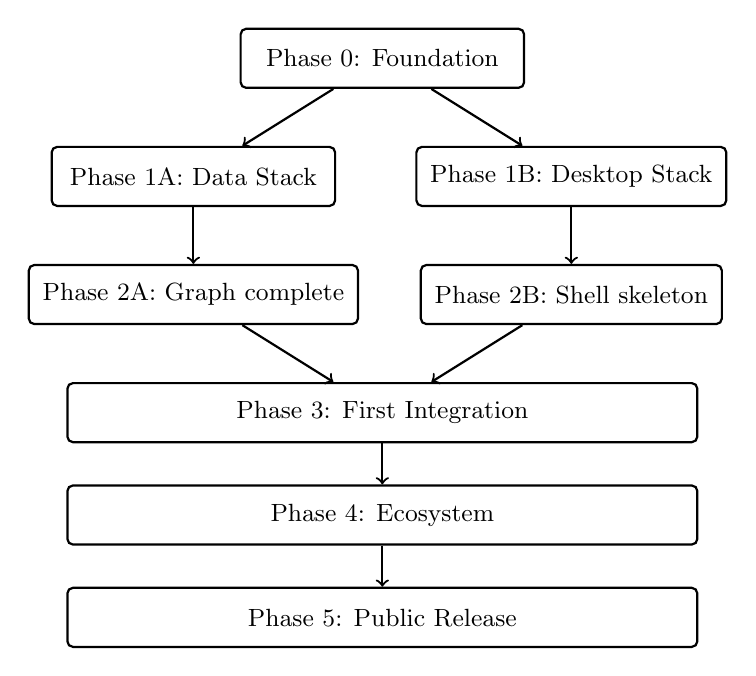
\begin{tikzpicture}[
  box/.style={
    draw, thick, rectangle, rounded corners=2pt,
    minimum width=3.6cm, minimum height=0.75cm,
    font=\small, align=center, inner sep=5pt
  },
  merge/.style={
    draw, thick, rectangle, rounded corners=2pt,
    minimum width=8.0cm, minimum height=0.75cm,
    font=\small, align=center, inner sep=5pt
  },
  arr/.style={->, thick},
  lbl/.style={font=\footnotesize\itshape},
]

\node[box] (p0)    at (0, 5.0)  {Phase 0: Foundation};

\node[box] (p1a)   at (-2.4, 3.5) {Phase 1A: Data Stack};
\node[box] (p1b)   at ( 2.4, 3.5) {Phase 1B: Desktop Stack};

\node[box] (p2a)   at (-2.4, 2.0) {Phase 2A: Graph complete};
\node[box] (p2b)   at ( 2.4, 2.0) {Phase 2B: Shell skeleton};

\node[merge] (p3)  at (0, 0.5)  {Phase 3: First Integration};
\node[merge] (p4)  at (0, -0.8) {Phase 4: Ecosystem};
\node[merge] (p5)  at (0, -2.1) {Phase 5: Public Release};

\draw[arr] (p0)  -- (p1a);
\draw[arr] (p0)  -- (p1b);
\draw[arr] (p1a) -- (p2a);
\draw[arr] (p1b) -- (p2b);
\draw[arr] (p2a) -- (p3);
\draw[arr] (p2b) -- (p3);
\draw[arr] (p3)  -- (p4);
\draw[arr] (p4)  -- (p5);

\end{tikzpicture}
\caption{Phase dependency structure. Phases~1 and~2 run as parallel tracks;
neither blocks the other. Phase~3 is the first point at which both tracks must
be simultaneously stable. Phases~4 and~5 are sequential.}
\label{fig:roadmap}
\end{figure}

Three types of milestone appear in each phase. \emph{Technical gates} are
binary, automatically verifiable conditions that must pass before the next
phase begins: a specific CI job is green, a benchmark hits a defined threshold,
or an interface check passes. \emph{UX milestones} are qualitative judgments
about usability that require a human to verify: a defined task completed
without assistance by a target user type. \emph{Sustainability milestones}
track organizational and community progress that runs in parallel with
technical development.

\paragraph{Phase 0: Foundation (current).}
Architecture and design decisions are documented in this blueprint. The
repository organization, CI template, and shared tooling are established before
component code is written. The base distribution is Fedora. The
\texttt{event-bus} protobuf schema is defined; the \texttt{sdk} crate structure
is initialized with the public API as traits before any implementation exists.
This ordering is intentional: schema and interface decisions are the most
expensive to change once downstream components exist.

\emph{Technical gates:} SQLite write store sustains 5,000 synthetic events per
second under continuous load without data loss; promotion pipeline moves events
into Ladybug and a Cypher query returns correct results; CI template deployed
and all initial repositories pass the required jobs; \texttt{just dev} starts
the Event Bus and Graph Daemon locally in under 10 seconds.

\emph{Sustainability milestones:} GitHub organization created with all
repositories; \texttt{foundation} repository public with this document;
ORCID and Zenodo record created for the architecture document.

\paragraph{Phase 1A: Data Stack.}
The eBPF Normalizer is operational, deduplicating and filtering raw kernel
events before they reach the Event Bus. The promotion pipeline is stable under
real desktop load, not only synthetic load. The Graph Daemon exposes a complete
Cypher query interface over its Unix socket. All components have integration
tests that run against real IPC sockets. The \texttt{knowledge} benchmark
suite is established and producing baseline measurements.

eBPF programs are developed and tested exclusively inside the QEMU developer
VM from this point forward. A bad eBPF program can produce a kernel panic; VM
isolation is mandatory, not optional.

\emph{Technical gates:} eBPF test job green in CI using nested QEMU on GitHub
Actions runners; integration test suite passes for the full pipeline from raw
eBPF event to Ladybug node; graph query latency baseline established for 1k,
50k, and 500k node datasets.

\paragraph{Phase 1B: Desktop Stack.}
The \texttt{compositor} repository is initialized as a standalone fork of
cosmic-comp with the COSMIC shell IPC removed and the custom Event Bus socket
added as the first patch in the series. The upstream tracking process is
operational: the weekly rebase CI job runs, and the patch series is clean
against current upstream. The compositor runs in nested mode inside an existing
Wayland session. No shell is connected yet.

\emph{Technical gates:} compositor starts in nested mode without crash;
upstream rebase CI job runs and produces no conflicts against current
\texttt{upstream/main}; patch series contains no more than five patches.

\paragraph{Phase 2A: Graph Complete.}
The full Knowledge Graph schema is implemented and stable. All node types
documented in Section~\ref{sec:knowledge-graph} exist and are populated by
real system activity. The temporal filesystem view at
\texttt{\textasciitilde/.timeline/} is functional. Retention policy and
summarization are implemented. The Graph Daemon is considered feature-complete
for the purposes of AI layer integration.

\emph{Technical gates:} all node types populated from a 24-hour real usage
session; \texttt{\textasciitilde/.timeline/} lists correct files for a
given date; retention pass runs and compacts nodes correctly.

\paragraph{Phase 2B: Shell Skeleton.}
The shell runs on the compositor fork. The taskbar, Waypointer (without graph
integration), the global menu bar, and the Appearance section of Settings are
functional. The theme system is operational: token-based switching propagates
to all Tauri surfaces and GTK4 applications. A developer can use this
environment as a basic desktop without requiring a terminal for routine tasks.

\emph{Technical gates:} Panda, Light, Dark, and High Contrast themes all
apply correctly and switch without a session restart; Waypointer launches
applications; the global menu bar renders menus from a first-party application.

\emph{UX milestone:} a developer who did not build the system can complete
five predefined tasks using only the shell, without referring to documentation.

\paragraph{Phase 3: First Integration.}
The two tracks are connected. Waypointer queries the Knowledge Graph for recent
files and project context. Focus Mode is fully implemented. The AI Daemon
operates with a local provider. The Connections system and Settings AI category
are functional. This is the first phase where the system is used as a daily
driver by the primary developer.

The daily driver criterion is not aspirational language. It is a concrete
testing strategy: running the system as the primary work environment for a
minimum of 30 consecutive days surfaces bugs and rough edges that no scripted
test scenario will find.

\emph{Technical gates:} Waypointer returns graph-sourced recent files
correctly; Focus Mode activates and deactivates all documented side effects;
AI Daemon responds to a graph query with a local provider configured.

\emph{UX milestone:} a non-technical test user completes a defined set of
daily tasks (web browsing, document editing, file management, calendar review)
without opening a terminal and without asking for help.

\emph{Sustainability milestones:} first public blog post or video documenting
the project; Sovereign Tech Fund and NLnet grant applications submitted.

\paragraph{Phase 4: Ecosystem.}
The Store is operational. The Install Daemon handles Integration Package
matching. The Module Runtime is functional. The first external developers are
onboarded with documentation and the \texttt{module-sdk}. Signed Profile
Packages for managed environments are supported. The project planning tool
decision is made and the chosen tool is in use.

\emph{Technical gates:} a Store application submitted by a developer outside
the core team installs and runs correctly end-to-end; a module declared in a
\texttt{.project} file activates and deactivates with Focus Mode.

\emph{UX milestone:} an external developer builds and submits a Store
application using only the published documentation, without asking the core
team for help.

\emph{Sustainability milestones:} first external contributor with a merged
pull request; Store infrastructure operational on Hetzner; first grant
funding received or first enterprise inquiry received.

\paragraph{Phase 5: Public Release.}
No new features. Hardware compatibility is validated against a defined target
list. The Nvidia first-boot detection and driver installation flow is tested on
real hardware. The installer is polished and the out-of-box experience meets
the bar set in Phase~3's UX milestone at scale. Documentation covers
installation, first use, and the most common troubleshooting scenarios.

\emph{Technical gates:} system tests green on release candidate ISO; Nvidia
driver flow completes without manual intervention on a tested device; installer
completes without errors on three distinct hardware configurations.

\emph{UX milestone:} a non-technical user installs the system from USB without
reading any documentation beyond the installer prompts, and reaches a working
desktop.

\emph{Sustainability milestones:} migration timeline from GitHub to
Forgejo/Codeberg defined; incorporation decision made based on available
funding and community size.


\clearpage

\clearpage

\printbibliography

\end{document}
